%%
%% This is file `thesis-ex.tex',
%% generated with the docstrip utility.
%%
%% The original source files were:
%%
%% uiucthesis2009.dtx  (with options: `example')
%% 
\def\fileversion{v2.25a} \def\filedate{2009/10/10}
%% Package and Class "uiucthesis2009" for use with LaTeX2e.
\documentclass[edeposit,fullpage]{uiucthesis2009}
\usepackage[usenames, dvipsnames]{color}
\usepackage{graphicx}
\usepackage{xspace}     %to get spaces in commands right
\usepackage{subfig}
\usepackage{url}
\usepackage{booktabs}
\usepackage{enumitem}
\usepackage{wrapfig}
\usepackage{lipsum}
\usepackage{caption}
\usepackage{multirow}
\usepackage{longtable}
\usepackage{amsmath}
\usepackage{rotating}
\usepackage{amssymb}
\usepackage{cancel}
\usepackage{colortbl}
\usepackage{xcolor}
\usepackage{notoccite}
\usepackage{units}      %to get proper nobreak spaces for units
\usepackage{hyperref}   %clickable links in pdfs
\usepackage{listings}
\usepackage{color}

\definecolor{dkgreen}{rgb}{0,0.6,0}
\definecolor{gray}{rgb}{0.5,0.5,0.5}
\definecolor{mauve}{rgb}{0.58,0,0.82}

\lstset{frame=tb,
	language=SQL,
	aboveskip=1mm,
	belowskip=1mm,
	showstringspaces=false,
	columns=flexible,
	basicstyle={\small\ttfamily},
	numbers=none,
	numberstyle=\tiny\color{gray},
	keywordstyle=\color{blue},
	commentstyle=\color{dkgreen},
	stringstyle=\color{mauve},
	breaklines=true,
	breakatwhitespace=true,
	tabsize=3
}

\nocopyrightpage

\newcolumntype{L}{>{\hspace*{-\tabcolsep}}c}
\newcolumntype{R}{c<{\hspace*{-\tabcolsep}}}
\newcommand{\ra}[1]{\renewcommand{\arraystretch}{#1}}
\colorlet{tableheadcolor}{gray!25} % Table header colour = 25% gray
\newcommand{\headcol}{\rowcolor{tableheadcolor}} %
\colorlet{tablerowcolor}{gray!10} % Table row separator colour = 10% gray
\newcommand{\rowcol}{\rowcolor{tablerowcolor}}

\newcommand{\CN}{\textcolor{red}{$^{[citation\ needed]}$}}
\newcommand{\Jpsi}{J/\Psi}
\newcommand{\us}{$\mu$s\xspace}
\newcommand{\red}[1]{\emph{\textcolor{red}{#1}}}
\newcommand{\bigoh}{\mathcal{O}}
\newcommand{\dbar}{\bar{d}}
\newcommand{\ubar}{\bar{u}}
\newcommand{\sbar}{\bar{s}}
\newcommand{\cbar}{\bar{c}}

\begin{document}

\title{Nuclear dependence of proton-induced Drell-Yan dimuon production at \unit[120]{GeV} at SeaQuest}
\author{Bryan P. Dannowitz}
\department{Nuclear Physics}
\schools{B.S., New Mexico Institute of Mining and Technology, 2008}
\phdthesis
\advisor{Naomi C. R. Makins}
\degreeyear{2016}
\committee{Professor Jen-Chieh Peng, Chair\\
	Professor Naomi C. R. Makins, Director of Research\\
	Professor Michael Stone\\
	Professor Jim Eckstein}
\maketitle

\frontmatter

%% Create an abstract that can also be used for the ProQuest abstract.
%% Note that ProQuest truncates their abstracts at 350 words.
\begin{abstract}
A measurement of the atomic mass ($A$) dependence of $p+A\rightarrow\mu^+\mu^- + X$ Drell-Yan dimuons produced by \unit[120]{GeV} protons is presented here. The data was taken by the SeaQuest experiment at Fermilab using a proton beam extracted from its Main Injector. Over 61,000 dimuon pairs were recorded with invariant mass $4.2 < M_{\gamma^*} < \unit[10] GeV$ and target parton momentum fraction $0.1\leq x_2 \leq 0.5$ for nuclear targets $^1H,\ ^2H,\ C,\ Fe,\ $and$\ W$. The ratio of dimuon yields per nucleon ($Y$) for heavy nuclei versus $^2H$, $R^{DY} = Y^{(A)} / Y^{(^2H)} \approx \bar{q}_u^{(A)}(x)/\bar{q}_u^{(^2H)}(x)$, is sensitive to modifications in the anti-quark sea distributions ($\bar{q}(x)$) in nuclei for the case of proton-induced Drell-Yan. The data analyzed here provides tighter constraints on various models that attempt to define the anomalous behavior of nuclear modification as seen in deep inelastic lepton scattering, a phenomenon generally known as the EMC effect.

\end{abstract}

%% Create a dedication in italics with no heading, centered vertically
%% on the page.

\begin{dedication}
Dedicated to my grandfather, Ted, who took me to school every day.
\end{dedication}

%% Create an Acknowledgements page, many departments require you to
%% include funding support in this.
\chapter*{Acknowledgments}

This dissertation comes as a grand sum of the help and support from the many colleagues, friends, and family in my life. First and foremost of them all, I give my thanks to my parents, Judy and Robert, who have never wavered in encouraging and supporting me in every way possible as I bounded through this long journey across many states, schools, jobs, and countries.

My sincere gratitude goes to my advisor and mentor, Naomi Makins, who first drew me to the University of Illinois and SeaQuest by her enthusiasm and fervor alone. Anything insightful that I may present or state here in this paper has probably come from what I have learned through her patient and exceptionally thoughtful teachings.

Thanks also go out to my fellow UIUC graduate students have been the bedrock of my academic life here. Without the constant cameraderie of my friend Evan McClellan, I fear I would not have made it through these past years with my sanity intact, and without the tenacious, creative, problem-solving mind of Bryan Kerns, I'm nearly certain that we would not have solved as many problems at SeaQuest as we have.

Particular thanks must extended to one, Markus Diefenthaler, who by sheer force of will held SeaQuest together and kept the collaborative effort focused for so many years. Markus also played a pivotal position as a role model to Evan, Bryan, and myself as what an experimental physicist should strive to be.

I would also like to state my appreciation to the SeaQuest collaboration for placing their trust (and data!) in the hands of a humble database administrator and second-year graduate student. I have learned very much in the company of the great scientific tapestry that is the SeaQuest collaboration, and I hope to carry all of the lessons I've learned with me throughout my life. Of course, the data presented here would simply not be possible without the grand coordinated efforts by all of the collaboration members to assemble and execute such an ambitious and challenging experiment.

My thanks also go out to the staff and faculty of the Nuclear and High Energy Physics Laboratory for their availability and willingness to help a graduate student in need. In particular, the weekly feedback and insight from Jen-Chieh Peng has been simply invaluable. The assistance from Steve Errede and Allison Sibert is the only reason that the PMT testing and development got off of the ground. Finally, life at the NPL would simply grind to a halt if it were not for the constant availability, willingness, and helpfulness of Mike Suchor.

I would also like to take a moment to thank the Department of Physice, the Nuclear Physics Laboratory, and the National Science Foundation\footnote{NSF Grant No. 1506416} for providing financial support and employ as a research assistant throughout the years, thereby giving me the opportunity to do something I love for a living.

Finally, I offer my most heartfelt gratitude to my wife, Carly, for the incredible leap of faith she took moving from Hawai`i on over to the middle of the corn fields just to be with me as I put myself through the rigors of these graduate studies. Her patience, understanding, companionship, and encouragement has truly been what has kept me going all these years.

%% The thesis format requires the Table of Contents to come
%% before any other major sections, all of these sections after
%% the Table of Contents must be listed therein (i.e., use \chapter,
%% not \chapter*).  Common sections to have between the Table of
%% Contents and the main text are:
%%
%% List of Tables
%% List of Figures
%% List Symbols and/or Abbreviations
%% etc.

\tableofcontents
\listoftables
\listoffigures

%% Create a List of Abbreviations. The left column
%% is 1 inch wide and left-justified
\chapter{List of Abbreviations}

\begin{symbollist*}
	\item[ACNET] Accelerator control system network
	\item[AD] Accelerator division (of Fermilab)
	\item[BIM] Beam intensity monitor
	\item[BNC] Bayonet Neill–Concelman signal cable connector standard
	\item[BOS] Beginning of spill
	\item[BPM] Beam profile monitor
	\item[CEBAF] Continuous Electron Beam Accelerator Facility
	\item[CODA] CEBAF On-line Data Acquisition
	\item[CS] Collins-Soper reference frame
	\item[CTEQ] Coordinated theoretical-experimental project on QCD
	\item[DAQ] Data acquisition
	\item[DC] Drift chamber
	\item[DIS] Deep-inelastic scattering
	\item[DY] Drell-Yan
	\item[EOS] End of spill
	\item[EOF] End of file
	\item[EPICS] Experimental physics and industrial control system
	\item[EVIO] CODA event input/output
	\item[FEE] Front-end electronics
	\item[FNAL] Fermi National Accelerator Laboratory (Fermilab)
	\item[FPGA] Field programmable gate arrays
	\item[IC] Ion chamber
	\item[LED] Light-emitting diode
	\item[LINAC] Fermilab Linear Accelerator
	\item[LO] Leading order
	\item[MI] (Fermilab) Main Injector
	\item[MOSFET] Metal–oxide–semiconductor field-effect transistor
	\item[NDF] Neutral density filter
	\item[NLO] Next-to-leading order
	\item[NM] Neutrino-muon beam line
	\item[NNLO] Next-to-next-to-leading order
	\item[PCB] Printed circuit board
	\item[PDF] Parton distribution function
	\item[PID] Particle identification
	\item[PMT] Photomultiplier tube
	\item[RF] Radio frequency
	\item[RFQ] Radio frequency quadrupole
	\item[ROC] Readout controller
	\item[SEM] Secondary emission monitor
	\item[SHV] Secure high voltage connector standard
	\item[SLAC] Stanford Linear Accelerator Center
	\item[SRC] Short range correlations
	\item[TS] Trigger supervisor
	\item[QCD] Quantum chromodynamics
	\item[QED] Quantum electrodynamics
	\item[QIE] Charge (Q) integrator and encoder
	\item[RDBMS] Relational database management system
	\item[SQL] Structured querying language
	\item[SWIC] Segmented wire ion chamber
	\item[VME] Versa Module Europa
\end{symbollist*}

\mainmatter

\chapter*{Preface}
\addcontentsline{toc}{chapter}{Preface}

Matters are rarely as simple as we hope them to be, and atomic nuclei are no exception. When physicists began to get a handle on proton structure, it was hoped that nuclei could be simply understood as a simple collection of the same familiar protons and neutrons. Unfortunately, it turned out that \emph{more is different}, and higher-order emergent behavior reared its head. It appeared that the distribution of partons within the proton became \emph{altered} when the proton was confined within a nucleus -- a phenomenon which is generally referred to as the EMC Effect. Since the discovery of this behavior, data and theories have proceeded to accumulate for over 30 years without a completely satisfying explanation, though recent breakthroughs give a reason for optimism.

The SeaQuest experiment was commissioned and began taking data in 2012 with the expressed purpose to, among other physics goals, shed some additional light on this phenomenon. I joined the collaboration in 2009 and have had the distinct pleasure of being a part of a large-scale, medium-energy experiment as it went from being an empty hall to a testing ground for nuclear physics. It has truly been a rewarding experience being able to contribute to a coordinated, monumental effort from the point of assembly all the way to its first publishable results (or at least very close). In this thesis, I will describe in detail these contributions to the experiment. 

Chapter 1 will provide a broad outline regarding the background to the underlying physics and phenomenology. I describe the state of the field regarding the physics of unpolarized sea quark distributions along with what SeaQuest can contribute. Emphasis is placed on the phenomenon of modification of the parton distribution functions when in the presence of a nuclear medium.

In Chapter 2, the apparatus of the SeaQuest experiment is laid out, briefly covering every significant aspect, including the beam, targets, magnets, detectors, and data acquisition systems. For further information on my contributions to the SeaQuest experiment's apparatus and operations, I have laid out in the following chapters my work on the curation of the collaboration's data productions (Chapter 3) and my work upgrading the hodoscope photomultiplier tube bases for improved performance (Chapter 4). These account for a significant amount of my own time and effort on the experiment but are \emph{not} required for understanding the background and analysis regarding the primary measurement of this paper.

Chapter 5 summarizes how the data used in these studies are reconstructed and selected. This includes a brief overview of the tracking algorithm that reconstructs tracks and dimuons from the raw detector readouts, and then a thorough rundown of the data reduction, showing in great detail how good events are chosen from the whole set.

In Chapter 6, I step through the many stages of the analysis, going from the raw reconstructed data all the way through the target-to-target normalization and a litany of corrections in order to arrive at a final result. Particular emphasis is placed on the corrections pertaining to the rate dependence, which has been the key obstacle in preparing preliminary results for all SeaQuest analyses. This section goes perhaps into more detail than needed, which is intentional, as this document is, in part, meant to act as an explanatory road map for future students and researchers who wish to perform this same analysis on the full SeaQuest dataset in the future.

Chapter 7 proceeds to summarize the fully processed and corrected findings, providing a comprehensive review of $R^{DY}$, the per-nucleon Drell-Yan cross section ratio of heavy nuclei to deuterium, against various kinematics. Results are briefly discussed and compared against theoretical predictions, though more refined corrections and more statistics from further SeaQuest data taking are required to come to any firm conclusions.

\chapter{Theoretical Background}

\red{CHAPTER STATUS: IN PROGRESS}

The topic of this paper is the exploration of the sub-structure of the \emph{nucleon}, a particle that makes up an atom's nucleus which can be either a proton (\emph{p}) or a neutron (\emph{n}). By sub-structure, I refer to the nucleon's composition and the momentum distributions carried by the nucleon's constituent particles, quarks and gluons.

While a complete review of the history and physics behind nucleon structure and its investigative probes is beyond the scope of this paper, a brief overview of Drell-Yan, parton distribution functions, and nuclear structure phenomenology will help in understanding concepts and terminology relevant to this and later chapters.

\section{Introduction}

The first indication that the proton may have some internal structure was in a 1933 experiment by Estermann \emph{et al.} measuring the magnetic moment of the proton \cite{Estermann:169E}. Since the proton was thought to be a point-like Dirac particle, it's magnetic moment ($\mu_p$) was expected to be $\mu_p = \frac{e}{2 m_p} = 1 n.m.$, or one \emph{nuclear magneton}. The experiment resulted in a value of 2.5 n.m., leading many to reconsider the notion that the proton is indeed point-like.

Around the same time, Hideku Yukawa is credited for establishing the first theory of a \emph{strong force}, a force binding together nucleons in a nuclei against the sizable \emph{Coulomb} repulsion of protons against each other. The force was theorized to be mediated by the exchange of particles called \emph{mesons}, and its range was limited to nuclei-scale distances, seeing as it's not observed at larger distances. Based upon the size of the nucleus, Yukawa estimated the mass of the intermediating particles to be approximately $2 \times 10^2 m_e \approx 100 MeV$, where $m_e$ is the electron mass. The following year, Anderson et al. discovered the muon ($\mu$) at around this mass\CN, which confused many as it did not seem to partake in strong interactions. Eventually, by 1947, the meson theory was validated by the discovery of the \emph{pion} by Powell \emph{et al.}\CN, and Yukawa was awarded a Nobel Prize for his theory in 1949. While the pion turned out to be just another composite particle, its discovery was a watershed moment in particle physics that led to a cascading series of discoveries. 
\begin{figure}
	\centering
	\includegraphics[width=4.5in]{figures/background/mesons_baryons.pdf}
	\caption{The octets and decuplet of Gell-Mann's ``Eightfold Way''. Top left: the eight particles of the meson octet; top right: the spin-$\frac{1}{2}$ baryon octet; bottom: the spin-$\frac{3}{2}$ baryon decuplet.}
	\label{fig:mesons-baryons}
\end{figure}

Near the end of the 1960's, SLAC began the first set of experiments to use an electron beam to investigate the nucleon in what is now known as Deep Inelastic Scattering (DIS). What they discovered was that the functions used to describe nuclear structure were largely independent of momentum transfer ($Q^2$) above a certain threshold. This so-called ``scaling'' behavior lent credence to the theory that nucleons were composed of a point-like particles. This discovery coupled with the proliferation of new particles (the ``particle zoo'') led Murray Gell-Mann and Yuval Ne'eman to construct a framework that would make some sense of it all. Gell-Mann had organized the host of mesons and baryons discovered into a geometric order named the ``Eightfold Way''\footnote{Gell-Mann here makes a rather poetic allusion to the Buddhist ``Noble Eightfold Path''} as depicted in Figure~\ref{fig:mesons-baryons}. The underlying explanation for all of this, as described independently by Gell-Man and Ne'eman, was to characterize these many particles as the several combinations of three \emph{flavors} of constituent particles, named \emph{quarks}. The flavors, \emph{u}, \emph{d}, and \emph{s} were named \emph{up}, \emph{down}, and \emph{strange}. Here, mesons were predicted to be composite particles of integer spin containing two quarks and baryons be half-integer spin particles composed of three quarks. This model led Gell-Mann to predict the existence of the $\Omega^-$ particle, along with its \emph{strangeness}, charge, and mass. The discovery of this particle\cite{1964PhRvL:12204B} earned Gell-Mann the 1969 Nobel Prize for his work on the quark model.

Though this model was a breakthrough in the understanding of fundamental particles, it did not comprehensively describe all experimental data. For example, when accounting for the total momentum of a nucleon, it was found that only $\sim50\%$ of the momentum was being carried by the quarks. It was not until the theory of quantum chromodynamics (QCD) came along that this and several other mysteries could be explained. QCD described the mechanism of a 3-fold \emph{color} charge and the gauge bosons, gluons, that intermediate the strong force between quarks (and other gluons). In the particular case of the missing momentum, this was found to reside in the intermediating gluons\cite{PhysRevLett.43.830}, which carry only color charge, to which the electro-weak probes used were insensitive.

Many nuclear probes and methods have been used to characterize the distributions and characteristics of nuclear partons, including the aforementioned DIS process. As I will describe later in this section, much has been learned about parton probability distribution functions with this and other processes, but it is the process of hadron-hadron di-lepton production that is of primary focus in this paper, which allows for an alternative approach to investigate the structure and characteristics of the quarks inside of a nucleon, and perhaps shed some light on some ongoing mysteries in nuclear physics.

\section{Di-lepton production in nucleon-nucleon collisions}

Studying the production of pairs of leptons resulting from hadron-hadron collisions has proven to be a powerful tool in probing nucleon structure and parton distribution functions (PDFs). Figure \ref{fig:DY-spectrum} shows the mass spectrum of the muon mode of di-lepton production in proton-nucleus collisions measured at the E-866/NuSea experiment at Fermilab\cite{PhysRevLett.80.3715}. The resonances of the $J/\Psi$, $\Psi^\prime$, $\Upsilon$, $\Upsilon^\prime$, and $\Upsilon^{\prime\prime}$ can be seen atop a smooth, continuous distribution which decreases with mass. The process responsible with this distribution of $\mu^+\mu^-$ pairs is the Drell-Yan process\cite{PhysRevLett.25.316}, which is illustrated in the Feynman diagram in Fig.~\ref{fig:dy-diagram}. This process is characterized by a quark annihilating with an anti-quark to form a virtual time-like photon which then decays into a pair of leptons. The study of this process can lend some insight into nucleon structure due to the fact that the mass and momentum of the di-lepton pair directly reflects the momentum distributions of the interacting quarks and anti-quarks. Current knowledge and models\CN of these momentum distributions come primarily from deep-inelastic lepton scattering (DIS) and the Drell-Yan (DY) process.

\begin{figure}
	\centering
	\includegraphics[width=4in]{figures/background/DY-spectrum-e866.png}
	\caption{Dimuon mass spectrum from E-866 $p+h$ collisions at \unit[800]{GeV/c}\cite{PhysRevLett.80.3715}.}
	\label{fig:DY-spectrum}
\end{figure}

%Di-lepton production has a record of being used as a technique for searching for new particles. 
One particular focus of study for the Drell-Yan process is its nucleon number-dependent (A-dependent) behavior of its cross sections. This is of particular interest due to a phenomenon known as the EMC effect, in which the European Muon Collaboration (EMC) discovered in 1983 that parton distribution functions become modified when in the presence of the nuclear medium. This A-dependent behavior was not expected for hard scattering processes as the modest (maximum $\unit[8.8]{MeV}$) binding energy of a nucleus on a nucleon was not thought to have a significant effect on quark momentum distributions within a nucleon (\unit[938]{$Mev/c^2$}). Many experiments since\CN have confirmed, extended, and precisely characterized the A-dependent behavior observed. Among the many hard scattering probes for investigating this phenomenon, the Drell-Yan process is uniquely capable of isolating the effect on the anti-quark distributions to a high degree of accuracy. The study of the effects of the nuclear medium on nucleon anti-quark distributions is the secondary research goal of the SeaQuest experiment and is the main focus of this thesis.

Within this thesis, the Drell-Yan process and its properties are discussed in \red{sections so and so} and various A-dependent behaviors seen in Drell-Yan and DIS are discussed in \red{sections so and so}. A few models are discussed in an attempt to theoretically characterize this A-dependent behavior in \red{sections so and so}.

In cases where a Drell-Yan process occurs, it can often be the case that the incident quark must pass through the strongly-interacting nuclear medium prior to its annihilation with the anti-quark in the target. By investigating the momentum distribution of the quark from the beam and it's A-dependence, some insight can be gained regarding the parton energy loss as it moves through a foreign nuclear medium. This topic and its existing data are briefly discussed in \red{section so and so}.

\subsection{The Drell-Yan Process}

\begin{figure}[h]
	\centering
	\includegraphics[width=5.0in]{figures/background/Drell-Yan.png}
	\caption{The Drell-Yan process, an $s$ channel interaction consisting of the annihilation of a quark with an anti-quark.}
	\label{fig:dy-diagram}
\end{figure}

The study of continuum di-lepton production in hadron collisions,
\begin{equation}
	h_A +  h_B \rightarrow l^+ l^- + X
	\label{eq:hh2ll}
\end{equation} 
can be used to study hadronic structure in a way that is complementary to the study of deep-inelastic scattering,
\begin{equation}
l + h \rightarrow l^\prime + X.
\label{eq:lh2lx}
\end{equation}
In 1970, S. Drell and T.M. Yan were the first to suggest that, at high $Q^2 (=M^2_{l^+ l^-}) \geq 16GeV^2$, the quarks inside the hadrons $h_A$ and $h_B$ can be considered free fermions in the instantaneous moment that they interact. The Drell-Yan model addresses the dominant subprocess here,
\begin{equation}
q_A + \bar{q}_B \rightarrow \gamma^* \rightarrow l^+ l^-
\label{eq:dy-process}
\end{equation} 
as an electromagnetic annihilation process. In this high-$Q^2$ kinematic space, the final state of the hadrons that contain these quarks becomes more or less irrelevant. By the energy-time uncertainty principle\CN of $\Delta E \Delta t \sim \hbar$, the timescales under consideration are $<10^{-25}s$, and the corresponding distances are $<10^{-17}m$, where the size of a nucleon is $\sim 10^{-15}m$\CN. At these short space-time scales, electromagnetic annihilation dominates this quark-quark interaction.

This is further reinforced by the widely accepted non-Abelian gauge field theory of Quantum Chromodynamics (QCD) which describes the interactions between quarks and gluons. QCD provides a theoretical justification for treating Drell-Yan processes as events isolated from the rest of the hadron states, and it does so through the concept of the running of the coupling constant, or \emph{asymptotic freedom}\cite{Bethke:2006ac}. This characteristic feature of QCD is described by the decrease of the strength of the strong force coupling constant as the space-time scale of the interaction approaches zero (i.e. as $Q^2 \rightarrow \infty$). The strong coupling constant can be expressed as a function of $Q^2$:
\begin{equation}
\alpha_s(Q^2) = \frac{1}{\beta_0 \ln (Q^2/\Lambda^2)}
\end{equation}
where
\begin{equation}
\beta_0 = \frac{12\pi}{33-n_f}
\end{equation}
Here, $\Lambda$ is the QCD scale parameter that depends on the number of quark flavors, $n_f$, and the renormalization scheme, measured to be around $\sim$ \unit[217]{MeV}. Experimental measurements of the running of the coupling constant as measured by many different processes can be seen in Figure~\ref{fig:asymptotic-freedom}.
\begin{figure}
	\centering
	\includegraphics[height=2.5in]{figures/background/asymptotic-freedom.jpg}
	\caption{A compilation of measurements of the running of the strong coupling constant, $\alpha_s(Q^2)$.}
	\label{fig:asymptotic-freedom}
\end{figure}

\subsection{Drell-Yan Kinematics}

In the center-of-mass frame, the Drell-Yan process can be broken down into three stages with three sets of kinematics (refer to Fig.~\ref{fig:dy-diagram}). Beginning with the quarks, \emph{x} is defined as the fraction of the hadron's momentum carried by the interacting quark or antiquark. Conventionally in fixed-target experiments, subscripts are assigned as $x_1$ and $x_2$, which refer to the quark/antiquark from the beam and the antiquark/quark from the target, respectively. This \emph{x} is called the Bjorken \emph{x}, and is well-known in DIS processes to have a value of
\begin{equation}
x = -q^2/2 p \cdot q
\end{equation} where \emph{p} and \emph{q} are the 4-momenta of the hadron and the photon.

The next stage of the process is the virtual photon. This photon' properties are effectively equivalent to the `dimuon' or `dilepton', which are the terms more commonly used in referring to kinematics. The first of its relevant kinematics is its mass $M_{\gamma^*}$, which represents its energy and virtuality. The value $x_F$, or Feynman-x, is the fraction of the maximum possible longitudinal momentum carried by the virtual photon in the beam direction. The transverse momentum, $p_T$, and the azimuthal production angle, $\phi_{\gamma^*}$ are the remaining kinematics associated with the virtual photon.

The third stage regards the pair of leptons produced. In the frame of the virtual photon, there is a polar and azimuthal decay angle, $\theta_\mu$ and $\phi_\mu$, respectively, for each of the decay muons. It becomes impossible, however, to reconstruct these variables, as the individual transverse momenta of the quarks are unknown, and the thus the quark-antiquark annihilation axis is unknown. This is remedied by shifting the process into the Collins-Soper (CS) reference frame\cite{PhysRevD.16.2219} which orients the reference axis to be parallel to the bisector of the angle between the interacting hadrons in the rest frame of the muon pair. A depiction of the Collins-Soper frame can be found in Fig.~\ref{fig:collins-soper}. In total, this brings a total of eight kinematic variables, summarized in Table~\ref{tab:var}.
\begin{figure}
	\centering
	\includegraphics[width=4.50in]{figures/background/collins-soper.png}
	\caption{A depiction of the Collins-Soper reference frame. The green plane along $\hat{h}$ is the plane shared by the two hadrons.}
	\label{fig:collins-soper}
\end{figure}

Experimentally, six independent variables are measured, which form a basis by which all eight can be known. This is due to the fact that two pairs of variables, ($M_{\gamma^*}$, $x_F$) and ($x_1$, $x_2$) are correlated by the following, ignoring quark masses and considering $p_\perp << p_{\ell}$:
\begin{eqnarray}
x_F & \equiv & \frac{p_{\ell}}{\sqrt{s}/2} \approx x_1 - x_2 \label{eq:xf=x1-x2} \\
M_{\gamma^*}^2 & \equiv & E^2 - p_{\ell}^2  = s x_1 x_2 \label{eq:m=sx1x2} \\
E & = & \frac{1}{2}(x_1 + x_2) \sqrt{s} \\
p_{\ell} & = & \frac{1}{2}(x_1 - x_2)\sqrt{s}
\end{eqnarray}
In this frame, the longitudinal momenta of the quarks are $x_1 \sqrt{s}/2$ and $- x_2 \sqrt{s}/2$, with $\sqrt{s}$ being the center of mass energy of the hadronic collision. So, by measuring the 3-momenta of the $\mu^+$ and $\mu^-$, the quantities ($M_{\gamma^*}$, $x_F$, $p_T$, $\phi_{\gamma^*}$, $\theta_\mu$, $\phi_\mu$), which is sufficient to calculate the remaining ($x_1, x_2$) in our approximation.

\begin{table}[h]
	\centering
	\begin{tabular}{c|r}
		Variable&Description\\ \hline \hline
		$x_{1/2}$ & Momentum fraction of the beam/target quark\\
		$M_{\gamma^*}$ & Mass of the virtual photon (dimuon)\\
		$x_F$ & Fraction of the max. possible $p_{\ell}$ carried by virt. photon\\
		$p_T$ & Transverse momentum carried by the virt. photon\\
		$\theta_{\mu}, \phi_{\mu}$ & Polar and azimuthal decay angle\\ & of one of the muons, in the CS ref. frame\\ \hline
		$\alpha$ & The fine structure constant \\
		$K(x_1,x_2)$ & High-order QCD correction term \\
		$\sqrt{s}$ & Center of mass energy of the hadronic collision \\
		$\sqrt{\hat{s}}$ & Center of mass energy of the $q\bar{q}$ collision \\
		$Q^{2}$ & Four-momentum of the intermediate time-like photon, squared \\ 
		$q_i^{t/b}(x)$ & The quark number density in the nucleon of the target/beam \\ \hline \hline
	\end{tabular}
	\caption{Kinematic variables relevant to the Drell-Yan process .}
	\label{tab:var}
\end{table}

\subsection{Cross-Section}

As the participating quarks are asymptotically free within each hadron, there will be no correlations between the probability distributions of the annihilating particles, and the process is independent of the distributions. As a result, the cross section of the Drell-Yan process can be reduced to a function of the electromagnetic annihilation process and the quark probability distribution functions. With these components and some QCD considerations, we can construct it piece by piece.

The first step is to begin with the known hard scattering cross section of $\epsilon + \bar{\epsilon} \rightarrow l^+ l^-$, where $\epsilon$ is an arbitrary particle. This cross section\cite{Halzen:1984mc} is given by
\begin{equation}
\sigma(\epsilon\bar{\epsilon}\rightarrow l^+l^-) = \frac{4 \pi \alpha^2}{3M_{\gamma^*}^2} e_f^2
\label{eq:annihilation-cross}
\end{equation}
where $\alpha$ is the electromagnetic fine structure constant, $e_f$ is the charge of the particle, and $M_{\gamma^*}$ is the dilepton mass. With this, we add the QCD consideration that only $q\bar{q}$ of opposite color can annihilate with each other into a colorless virtual photon. Possible combinations are $R\bar{R}$, $B\bar{B}$, and $G\bar{G}$ out of $3\times 3$ possible cases. As such, an overall factor of $\frac{1}{3}$ is added to this cross section. Finally, factoring in the conservation of flavor (there can only be $u\bar{u}$, $d\bar{d}$, etc. combinations) and the quark structure of hadrons A and B,  we use the product ($q_f^A(x_1)\bar{q}_{f}^B(x_2)$) of the quark probability distributions for finding quarks of the same flavor-antiflavor combination in the two hadrons. It must also be considered that the quark or antiquark may be found in either hadron A or hadron B. The product of these three factors leads us to the Drell-Yan cross section\cite{Drell:1970wh}
\begin{eqnarray}
\frac{d^2\sigma}{dx_1dx_2}&=&\frac{1}{3}\frac{4\pi\alpha^2}{3M_{\gamma^*}^2}
\sum_{f}e_f^2[q_f^A(x_1)\bar{q}_f^B(x_2)+
\bar{q}_f^A(x_1)q_f^B(x_2)]\\
&=&\frac{4\pi\alpha^2}{9 s x_1 x_2}
\sum_{f}e_f^2[q_f^A(x_1)\bar{q}_f^B(x_2)+
\bar{q}_f^A(x_1)q_f^B(x_2)]
\label{eq:DY-cross}
\end{eqnarray}
where the sum is summing over flavors of quarks ($f\in\{u,d,s,...\}$). This can be evaluated in terms of the measurables $M_{\gamma^*}$ and $x_F$ via Equations~\ref{eq:xf=x1-x2}~and~\ref{eq:m=sx1x2}
\begin{equation}
M_{\gamma^*}^2 \frac{d^2\sigma}{dM_{\gamma^*}^2 dx_F} = 
\frac{1}{3}\frac{4\pi\alpha^2}{3M_{\gamma^*}^2}
\frac{x_1 x_2}{x_1 + x_2}
\sum_{f}e_f^2[q_f^A(x_1)\bar{q}_f^B(x_2)+
\bar{q}_f^A(x_1)q_f^B(x_2)]
\label{eq:dy-cs-observe}
\end{equation}
where $x_1$ and $x_2$ can be expressed as
\begin{equation}
x_1 = \frac{1}{2}\left[\sqrt{x_F^2 + 4\tau} + x_F\right],\ \  
x_2 = \frac{1}{2}\left[\sqrt{x_F^2 + 4\tau} - x_F\right],\ \ 
\tau = \frac{M_{\gamma^*}^2}{s}
\end{equation}
The cross section can also be represented by dimensionless variables in its scaling form,
\begin{equation}
s \frac{d^2\sigma}{d \sqrt{\tau} dy} = 
\frac{1}{3}\frac{4\pi\alpha^2}{3}
\sum_{f}e_f^2[q_f^A(x_1)\bar{q}_f^B(x_2)+
\bar{q}_f^A(x_1)q_f^B(x_2)]
\label{eq:dy-cs-dimensionless}
\end{equation}
where we introduce the rapidity term $y$ in describing $x_1$ and $x_2$,
\begin{equation}
y  = \frac{1}{2} \ln \frac{E+ p_\ell}{E-p_\ell} = \frac{1}{2} \ln \frac{x_1}{x_2},\ \ 
x_1  = \sqrt{\tau} e^{y},\ \  
x_2  = \sqrt{\tau} e^{-y}
\end{equation}
It should be noted that with collider experiments, it is conventional to refer to the hadrons A and B in terms of the beam and target hadrons, respectively, and as such, $x_1$ refers to the the quark in the beam hadron and $x_2$ refers to the quark in the target hadron.

In each of these equations~\ref{eq:DY-cross}, \ref{eq:dy-cs-observe}, and \ref{eq:dy-cs-dimensionless}, the cross sections can be factored into two parts: one subprocess cross section and one part that has only a dependence on the parton distribution functions. They are independent of each other, because one of the staples of the quark parton model is that the PDFs ($q(x) and \bar{q}(x)$) are independent of the process by which they are probed. At this point, let's look a bit more deeply into these PDFs, how they're measured, and their behavior.

\subsection{The Quark Parton Model and PDFs}

%Let's say that we have two hadrons A and B colliding; a parton of type \emph{a} ($u, d, s, g$, etc.) comes from A and carries with it a fraction of A's momentum ($x_A$).  The same goes for hadron B; a parton of type \emph{b} comes from B and carries momentum fraction $x_B$. Now, the probability of finding the discussed parton from A is given by $f_{a/A}(x_A)dx_A$. Likewise, the probability of finding the discussed parton from B is $f_{b/B}(x_B)dx_B$.  
%
%These \emph{structure functions}, $f_{a/A}(x)$ are called the \emph{parton distribution functions} (PDF's), and they have been the focus of a great deal of experiments over the years by several collaborations. Due to the complex nature of lattice QCD, these PDF's are determined empirically, with only a few rules based in theory. It is important to note that there is normally a $Q^2$ dependence of these PDF's. At high enough $Q^2$, as it is in the case of our experiment, the PDF's no longer scale with $Q^2$ \cite{Seely:2009gt}.  That is, for a given \emph{x}, the PDF is independent of $Q^2$.
%
%An important metric to observe is the probability that a parton \emph{a} carries a momentum fraction $x_A$ in its hadron $A$.  This can be represented by the following expression: $x_A f_{a/A}(x_A)dx_A$. For Drell-Yan interactions in the study proposed here, we are interested in the momentum distribution amongst the quarks in the proton.  The CTEQ collaboration has collected data from many experiments, yielding the model represented in Figure \ref{fig:pdf} \cite{Pumplin:2002vw}.
%
%\begin{figure}
%	\centering
%	\subfloat[][The parton distribution function describing the momentum carried by different types of quark in the proton.]{%
%		\label{fig:pdf}%
%		\includegraphics[width=0.40\linewidth]{figures/background/parton-dist.jpg}}%
%	\hspace{8pt}%
%	\subfloat[][The ratio of cross sections (per nucleon) as a function of the target's fractional momentum, $x_2$.  The EMC Effect region, $0.3<x_2<0.6$ is the phenomenon discussed here.]{%
%		\label{fig:emc}%
%		\includegraphics[width=0.53\linewidth]{figures/background/EMC_EMC.jpeg}}
%	\caption{The proton's momentum distribution and the EMC Effect, with key regions highlighted.}
%	\label{fig:pdf_emc}
%\end{figure}
%
%Looking to Figure \ref{fig:pdf} we see that at $x>0.1$, $u$ and $d$ quarks dominate $\bar{u}$ and $\bar{d}$ quarks.  This is key, because this means that, for SeaQuest where we have high $x_1$ and lower $x_2$, the Drell-Yan process is probabilistically dominated by a quark from the beam annihilating with an antiquark from the target. All antiquarks that exist in the target nucleons must come from what are called the \emph{sea quarks}, or the virtual $q\bar{q}$ pairs that pop in and out of existence amongst the gluons and valence quarks. 
%
%As we will discuss in the next section, partons in a bound nucleon behave differently than partons in a free nucleon. By studying Drell-Yan in nuclear targets, we can investigate the degree to which this modification is the result of a modification to the quark sea.
%

\subsection{QCD-Improved Drell-Yan and the K-Factor}

%In addition to the leading-order DY term, there are high-order QCD corrections to consider. These have been studied and accounted for up to $\bigoh(\alpha_s)$ and $\bigoh(\alpha_s^2)$. These include contributions from high-order $q\bar{q}$ annihilation $(q \bar{q} \rightarrow \gamma * + g)$ and gluon Compton scattering $(q + g \rightarrow \gamma * + q)$ as seen in Figure \ref{fig:nlo-dy} \cite{duan-2007-50}. The cumulative effect is denoted in the cross section as the $K(x_1,x_2)$ factor, which can vary between 1.6 and 2.8.  For our $x_1$ and $x_2$ range, $K \sim 1.6$.

\begin{figure}[h]
	\centering
	\includegraphics[width=5.00in]{figures/background/DY.jpeg}
	\caption{The Drell-Yan process has a large range of higher-order QCD corrections that need to be accounted for. 
		(A) and (B) are high order $q\bar{q}$ annihilations, and (C) and (D) are gluon ``Compton scattering'' terms.}
	\label{fig:nlo-dy}
\end{figure}

\section{Drell-Yan in Nuclei}

\subsection{The EMC Effect}

%The European Muon Collaboration, in 1983, measured the DIS cross section per nucleon ratios of $Fe$ to $D$ over a large kinematic range.  The result, as seen in the top right of Figure \ref{fig:emc} came as quite a surprise.  It was revealed that the structure function of a nucleon bound in a nucleus differs fundamentally from that of a free nucleon  \cite{Aubert:1983xm}.  This difference was not a simple or small effect either; the cross section per nucleon of a nucleus showed to be smaller than that of deuterium at very low $x_2$, greater than deuterium at $0.1<x_2<0.2$, and then steadily less than deuterium for $0.2<x_2<0.6$. 
%
%This complex, unexplained behavior opened up a new field of research and theoretical work. Following suit, the different aspects of this nuclear modification garnered some common nicknames.  The region where $x_2<0.1$ became known as \emph{``Nuclear Shadowing''}, the transition region of $0.1<x_2<0.2$ is known as \emph{"Anti-shadowing"}, and the linear decline in the ratio of cross sections between $0.2<x_2<0.6$ is generally referred to as the \emph{"EMC Effect"} \cite{Geesaman:1995yd}.
%
%The phenomenon was simple -- DIS off of a bound nucleon was not the same as off of a free nucleon -- but hundreds of theoretical papers were written attempting to explain it away, from multiquark ($6q$) clusters to the exchange of virtual pions in the nucleus. Some have joked that EMC should stand for \emph{"Every Model is Cool"}. The focus of recent work (and this paper) is on the ``EMC Effect'' region, characterized by the distinctly linear downward slope.
%
%Recent experiments at Hall C at JLab and SLAC suggest the following regarding the EMC Effect \cite{Seely:2009gt}:
%\begin{itemize}
%	\item
%	It is $Q^2$-independent
%	\item
%	It's x-dependent shape is universal (across various nuclei)
%	\item
%	The magnitude (slope) of the effect varies with A
%	\item
%	It thereby might be related to nuclear density
%\end{itemize}
%
%In parallel to this effort, many researchers were working on high-momentum nucleons and short range correlations (SRC's), neither aware yet of their common ground.

\subsection{Models For the EMC Effect}

\subsubsection{Pion Cloud Model}

\subsubsection{Nuclei-Nuclei Short Range Correlations}

\subsection{E-772 at Fermilab}

\chapter{Apparatus}

SeaQuest is the operational name of Fermilab Experiment \#906 (\emph{E-906}) performed at its Neutrino-Muon (\emph{NM})
experimental area. The experiment was designed
to take \emph{high-intensity beam} at relatively \emph{low center-of-mass energy}, provide
\emph{good mass resolution}, and allow for \emph{accurate target-to-target systematic normalization}.
The apparatus consists of a moving target table, two dipole magnets, 8 hodoscope planes, 24 drift 
chamber planes, and 4 proportional tube planes. Upstream of the target table (towards the beam source),
there is also a Cherenkov counter for beam intensity monitoring and there are
several segmented wire ionization chambers (SWIC's) for beam profiling.

\section{Apparatus Overview}

SeaQuest is a fixed-target experiment. In this style of
experiment, a stationary target is placed in the path of an accelerated beam of particles, as opposed to \emph{collider} 
experiments where two accelerated beams are directed against each other, in opposite directions. The proton beam
interacts with the target material and produces a variety of daughter particles. These daughter particles are 
tracked through a forward spectrometer and selectively filtered dependent on the purpose of the study.

The tuned and monitored 120 GeV proton beam is sent from the Fermilab Main Injector (MI) where the beam
protons strike one of the 7 targets. The high-momentum charged particles that are produced are focused
onto the various detectors with the solid iron dipole magnet, FMAG, or NM3S. 
This solid focusing magnet also sweeps away low-momentum particles and acts as a beam dump / absorber.

\begin{figure}
	\begin{center}
		\includegraphics[width=0.75\textwidth]{figures/Spectrometer.png}
		\caption{Perspective view of the SeaQuest spectrometer apparatus.}
		\label{fig:spectrometer-perspective}
	\end{center}
\end{figure}


The SeaQuest Spectrometer (Fig. \ref{fig:spectrometer-perspective}) consists of a focusing magnet to bend charged particles into the experiment's acceptance,
several tracking chambers that record the positions of charged particles through the length of the spectrometer, and
an analyzer magnet to bend the particles between tracking stations. The spectrometer measures particle momenta by
recording the bend of each charged particle as it passed through the analyzer magnet, where the magnetic field is known.
This is performed by reconstructing the trajectory of a particle in one half of the spectrometer (before the
analyzer magnet) and then similarly reconstructing the trajectory of particles in the other half. If two 
trajectories can be matched up, then the particle momentum can be extracted by taking the ratio of the 
magnet's $p_T$-kick to the change in the track's direction.

The spectrometer geometric design and event
triggering selection is optimized to detect oppositely-charged pairs of muons while minimizing the sensitivity
to various sources of unwanted backgrounds. Positive identification of muons is achieved by requiring signals
in the hodoscopes for known muon \emph{``roads''} along with requiring signals in the proportional tubes located at
the farthest end of the experiment, past an iron wall. Electrons and any hadrons are stopped by the solid iron
focusing magnet an iron wall further down, while muons will pass through them unencumbered.

The coordinate system is defined as the following: the \emph{z}-axis points along the beam direction, the
\emph{y}-axis points upwards vertically, and the \emph{x}-axis lies along the horizontal direction
in such a way that a right-handed coordinate system is formed. The terms \emph{upstream} and 
\emph{downstream} are often used when referring directions or regions in the experimental hall.
\emph{Upstream} often refers to the region of the experiment towards the beam source, while
\emph{downstream} refers to everything towards the $+z$ direction. 
The The origin of the coordinate system was chosen to be the point where the proton beam meets 
the \emph{upstream}-facing surface of FMAG, the solid focusing magnet.


\section{Main Injector Proton Beam}

%% January 7th begin

The Fermilab Main Injector (MI) receives protons that have been accelerated by the Radio Frequency Quadrupoles (RFQ), 
the Linear Accelerator (LINAC), and the Booster, and it continues to accelerate them from 8 GeV up to the nomimal energy
of 120 GeV. Along the way, the radio-frequency cavity (RFC) accelerators in the LINAC and the MI ``bunches'' up the
protons such that the beam has its characteristic 53.1 MHz structure. After the period of acceleration, the protons
are then 'scraped off' slowly with each passing \emph{turn} of the collected proton beam and sent down the
Neutrino-Muon (NM) beam delivery line for approximately five seconds of every minute, called a ``slow spill'', or just
``spill''. Beam is extracted using a resonant process, and the extracted beam retains the 53.1 MHz structure of the
Main Injector RFC. Each bunch, or ``bucket'' of protons is less than 2 ns long and the time between bunches is approximately
18.8ns. The spill structure of the beam is depicted in greater detail in Figure \ref{fig:SpillStructure}.

\begin{figure}
	\begin{center}
		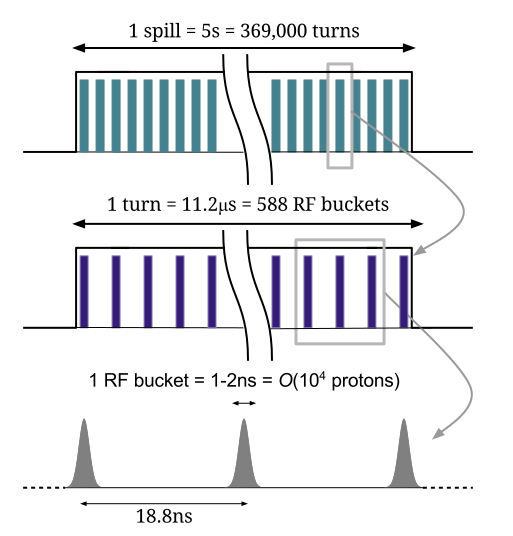
\includegraphics[width=0.55\textwidth]{figures/SpillStructure.pdf}
		\caption{Spill structure of the beam delivered to SeaQuest.}
		\label{fig:SpillStructure}
	\end{center}
\end{figure}

The beam sent to SeaQuest is not uniform in time throughout the spill (in more ways than one).  There are beam bunches in the
MI that are intentionally left empty so that the abort kickers can ramp to full field during a gap in the beam. There are also
bunches left empty to allow the injection kickers to inject 8 GeV protons from the Booster without disturbing bunches of protons
already in the Main Injector.  Typically, 498 of the 588 ``RF buckets'' in the Main Injector contain protons during the SeaQuest
slow spill cycle.  It is the case, however, for SeaQuest, that the intensity of the bunches corresponding to these 498 full
buckets varies greatly throughout the slow spill. On \emph{average}, each bucket will have \emph{O}($10^4$) protons, and the spill
has an intensity of approximately $2\times 10^{12}$ protons per second and therefore about $1\times 10^{13}$ protons delivered per spill.

Several guiding and focusing magnets bend and deliver beam to the NM beamline which serves both the test beam facility and SeaQuest at NM4.
The beam is focused to a width of 250$\mu$m. The profile, position, and intensity are measured along the NM beamline by several detectors.
The intensity of the beam is monitored by an ion chamber (IC) and a secondary emission monitor (SEM) in the NM3 sector. The beam profile
and position are monitored by SWICs and beam-position monitors (BPMs), respectively. The Accelerator Control Network
(ACNET) display of the SWIC readout can be seen in Figure \ref{fig:Profile}. The closest BPMs and SWICs to the spectrometer were
located in NM2 enclosure. The beam profile does not maintain its 250$\mu$m shape, and spreads slightly as it moves towards the
spectrometer. The final beam profile is measured by inspecting the upstream-facing side of the solid targets, and it was found
to be approximately 6mm wide by 1mm high.

\begin{figure}
	\begin{center}
		\includegraphics[width=0.65\textwidth]{figures/swic.jpg}
		\caption{Beam profile detailed by SWIC detectors along the NM beam line.}
		\label{fig:Profile}
	\end{center}
\end{figure}

\section{Beam Intensity Monitor}

SeaQuest's trigger system (described in detail later) mostly fires on fake dimuons caused by two low $p_T$ muons from
unrelated pion decays. The hits in downstream hodoscopes from the pions combined with hits in the upstream
hodoscope from two other unrelated particles frequently add up to a false dimuon signal. Since this type of fake
trigger involves four unrelated particles, the probability that a trigger will occur increases with $I^4$, where
$I$ is the intensity of the beam bucket, or the number of protons in the triggered beam bunch.

The SeaQuest data acquisition system (also described later in detail) can read out approximately 3000 events per
second without significant dead time.  During the commissioning run of SeaQuest, the trigger rate was very high and the
trigger dead time was close to 100\%.  These triggers were taken at such high beam intensities that the occupancy
of all SeaQuest detector elements was more than 50$\%$, making pattern recognition essentially impossible
(see Figure. \ref{fig:splat}). The Beam Intensity Monitor (BIM) was designed to solve this problem.

\begin{figure}
	\begin{center}
		\includegraphics[width=0.5\textwidth]{figures/splat2.png}
		\caption{A single high-intensity event with majority of all detector elements firing off. White space within the rectangles indicates inactive elements whereas red, blue, and green represent elements which have fired during that event. Track reconstruction in these cases is impossible.}
		\label{fig:splat}
	\end{center}
\end{figure}

The SeaQuest Beam Intensity Monitor (BIM) senses when the beam intensity is above a programmable threshold.
If an RF bucket with an intensity above this threshold is detected, the BIM sends a signal to inhibit
certain triggers until the intensity once more falls below the threshold. The inhibit threshold is tuned
frequently as trigger and beam conditions change, but the inhibit threshold is typically set at approximately
95,000 protons per RF bunch. For reference, a full RF bucket at an intensity of $2\times 10^{12}$ protons per
spill is $\approx$10,000 protons.

The beam intensity is measured using an atmospheric pressure gas Cerenkov counter. A gas mixture of 80$\%$ Argon and 20$\%$ CO$_2$
is used as the Cerenkov radiator. The counter and readout electronics were designed to have $O(ns)$ time resolution, and a linear
response over a large dynamic range.  A diagram of the counter is shown in Figure~\ref{fig:BIMCerenkov}.  A 45 degree aluminized
Kapton mirror directs light to a single photomultiplier tube.  A \emph{baffle} of black construction paper held parallel to the
mirror ensures that the proton path length through the light-radiating gas with respect to the mirror is independent of beam
position. A two-inch diameter 8-stage photomultiplier tube (PMT) is positioned close to the mirror so that all Cerenkov light created between the baffle and the mirror falls directly on the aperture of the PMT. It was observed during the commissioning run
that after exposure to $\approx 3 \times 10^{17}$ protons (~3 weeks of uninterrupted usage), the mirror reflectivity is significantly reduced in the beam spot, and the mirror then needs to be replaced.

\begin{figure}
	\begin{center}
		\includegraphics[width=0.6\textwidth]{figures/BIMCerenkov.pdf}
		\caption{The Beam Intensity Monitor (BIM) Cerenkov counter. Measurements are in inches.}
		\label{fig:BIMCerenkov}
	\end{center}
\end{figure}

The signal from the BIM is integrated and digitized using a custom charge (Q) integrator and encoder (\emph{QIE}) integrated circuit board, which comes from a family of circuits used first by the KTeV experiment at Fermilab\cite{QIE}. The chip is clocked with the Main Injector RF clock and provides an ADC (analog-digital conversion) every 18.8ns clock cycle. The light incident on
the photomultiplier tube is attenuated using neutral density filters (NDF's) so that the QIE least count corresponds to
$\sim$30 protons per beam bunch.

In addition to inhibiting triggers during high-intensity periods of beam, the BIM readout module also provides critical
information used to calculate the number of protons incident on the SeaQuest targets while the experiment is ready
and able to trigger. This value is needed to normalize SeaQuest cross section measurements. The BIM readout module provides the following:
\begin{itemize}
\item Sum of all ADC signals for the entire spill (QIESum).
\item Sum while inhibit is asserted at trigger logic.
\item Sum during trigger dead time.
\item A snapshot of beam intensity 16 buckets before and after the triggered RF bucket
\end{itemize}

These are used to calculate a ratio of protons that were `live' (the experiment can trigger) via the following:
\begin{eqnarray}
	liveRatio & = & \frac{QIESum - (inhibit\ sum + dead\ time\ sum)}{QIESum} \\
	liveProton & = & totalProton \cdot liveRatio
	\label{eqn:liveproton}
\end{eqnarray}
where ``totalProton'' is the intensity value recorded from the SEM detector located just upstream of the BIM Cerenkov counter.
The SEM itself is calibrated by foil activation. The snapshot of the triggered RF bucket intensity along with the 32
surrounding RF bucket intensities is used for studies and corrections of the rate-dependent effects on detector efficiencies
and reconstructed measurements.

\section{The SeaQuest Targets}

\begin{table}[p]
	\begin{center}
		\begin{tabular}{c c c c c c c}
			\parbox{1.5cm}{\centering{~\\Position} } & \parbox{1.5cm}{\centering{~\\Material} }  &\parbox{1.5cm}{\centering{Density\\{[g/cm$^3$]}} }  &  \parbox{1.75cm}{\centering{Thickness\\{[cm]}} }& \parbox{2cm}{\centering{Interaction\\Length} }&  \parbox{1.5cm}{\centering{Spills/\\Cycle\\(\%spills)} } \\ [0.5ex] \hline
			1 & $H_2$     & 0.07065 & 50.8  & 0.06902 & 10 (43\%) & \\
			2 & Empty     & NA      & NA    & 0.0016  & 2 (9\%)  & \\
			3 & $D_2$     & 0.1617  & 50.8  & 0.1144  & 5 (22\%)  & \\
			4 & None      & NA      & NA    & 0.0     & 2 (9\%)  & \\
			5 & Iron      & 7.874   & 1.905 & 0.1135  & 1 (4\%)  & \\
			6 & Carbon    & 1.802   & 3.322 & 0.0697  & 2 (9\%)  & \\
			7 & Tungsten  & 19.30   & 0.953 & 0.0958  & 1 (4\%)  & \\ [0.5ex] \hline
		\end{tabular}
		\caption{Characteristics of the seven SeaQuest target positions.  The ``Spills/Cycle'' is only a typical configuration and can vary according to needs and running configurations.  The non-zero interaction length of the empty flask is due to the 51$\mu$m-thick stainless steel end-caps of the flask and the 140 $\mu$m-thick titanium windows of the vacuum vessel that contains it.}
		\label{tab:target-materials}
		
	\end{center}
\end{table}

\begin{figure}[p]
	\begin{center}
		\includegraphics[width=0.65\textwidth]{figures/target-tableLayout.pdf}
		\caption{The layout of the target table and its seven target positions, as seen from above.}
		\label{fig:table-layout}
	\end{center}
\end{figure}


A wide range of atomic weights (from 2 to 184) is required to do an A-dependence study of the Drell-Yan process.
At SeaQuest, the targets used are $^1H (\ell),\ ^2H (\ell),\ C,\ Fe,\ $and$\ W$. In addition to the two liquid targets
and the three solid targets, two positions on the target table were used for measuring background signal rates:
an empty flask, identical to the flasks used for the $^1H$ and $^2H$ targets, and a single empty solid target holder.
Colloquially speaking: the $^1H$ target is interchangeably referred to as the liquid hydrogen target, $\ell H_2$,
\emph{LH2}, or $H_2$; $^2H$ is likewise referred to as the liquid deuterium target, $\ell D_2$, \emph{LD2}, or $D_2$;
the empty flask is referred to as the ``Empty'' target; the empty solid target holder is referred to as the ``None'' target.

These are all mounted on a laterally-moving, remotely positionable table (in the $\pm x$ direction), able to move
over a range of 91.4cm. The table's center is located at $(0, 0, -1.25)$ meters, directly in front of the upstream face
of FMAG, the solid iron focusing magnet. Because of the $\sim$5.0cm diameter of the targets and the 6x1mm dimensions of the beam, the targeting efficiency was 100\%. The details of the target materials are summarized in Table \ref{tab:target-materials}, and the layout of the target table can be seen in \ref{fig:table-layout}.

The $H_2$ gas used is ``Ultra High Purity 5.0 Grade'' or 99.999\% pure.  The deuterium has come from two different
sources.  The first of these is Fermilab-provided supply of gas left over from previous bubble chamber experiments.
This gas was known to have a small hydrogen contamination and was measured by mass spectroscopy to have a composition
of 85.2\% D$_2$, 12.7\% HD, 1.2\% $^4$He, and 0.8\% H$_2$ by mole. As analysis of experimental data commenced, 
handling the ramifications of the D$_2$ impurity came under focus. Unexpected bottle-to-bottle variation in contamination
became evident, and the sample-taking methodology itself for spectroscopy became suspect of introducing contamination.
In order to no simplify analysis and reduce the substantial complexity and cost of further gas analysis, SeaQuest switched
to commercially available ``Research Grade'' D$_2$, which is better than 99.6\% pure with virtually all HD to balance.
The data analyzed in this paper deals with the impure D$_2$ target material before this switch. Further information on
the D$_2$ composition and how it is handled in analysis will be covered in Chapter 4.

%10'' apart to approximate the 20'' 
%  more closely spaced (6.73'').

Each of the three solid target positions is divided into three disks of 1/3 the total thickness provided in Table \ref{tab:target-materials}. These disks are spaced 25.4cm apart to approximate the distribution of the liquid target, thereby minimizing target-dependent variation in spectrometer acceptance. The one exception to this is that during the Run II period the iron plugs were more closely spaced (17.1cm). The decision to place these
iron disks closer together than the rest during Run II is still unclear.

The target table is able to move between two different targets in about 30 seconds. This allows a change in target in the 55 seconds between successive spills. With this frequent target interchange, the systematic uncertainties associated with drifts in beam characteristics, monitor gains, and detector efficiencies are reduced to a minimum when investigating A-dependent ratios. How much beam time each target received is determined by interaction lengths of the targets along with the amount of statistics desired for certain targets. As the flagship measurement of SeaQuest is the $\bar{d}/\bar{u}$ asymmetry, more emphasis was placed on the hydrogen and deuterium than the nuclear targets. The spills per cycle and beam time allocation can be found in Table \ref{tab:target-materials}.

\section{Focusing and Analyzing Magnets}

Two large dipole magnets are used in the experiment to be select forward going ($x_F > 0$) dimuons, reject low-momentum particles, and analyze their kinematic characteristics. The most upstream magnet, denoted ``FMAG'', is a solid iron A-frame magnet with an aperture of 1.22m in the $x$-direction and 66cm in the $y$-direction. It is assembled from 43.2cm x 160cm x 503cm iron slabs, as shown in Fig.~\ref{fig:FMag}. The magnet has no air gap, and the iron has extremely high purity, allowing a 2000A excitation current to generate a nearly constant, central magnetic field of 1.9 Tesla (yielding a 2.91 GeV/c total magnetic deflection). The field is generated by exciting the embedded aluminum \emph{``bedstead''} coil to 2000 Amps at 25 Volts (50 kW).  The current exciting FMAG is monitored by the Fermilab ACNET system and is broadcast to the SeaQuest slow data acquisition system every acceleration cycle. The excitation is also input to the beam-disabling safety system in order to prevent beam from hitting the SeaQuest spectrometer when FMAG is not fully powered. FMAG also acts as the beam dump for the 120 GeV beam. There is a 5cm diameter by 25cm deep bore drilled into the upstream end of FMAG (recall, this is the origin of the experiment's coordinate system).  The 120 GeV protons that do not interact in the SeaQuest targets 125cm upstream of FMag, interact in the central iron slab.  Most of the 2.0 kW beam power is dissipated in this slab and is eventually conducted to the coils and external surfaces to be radiated away.

\begin{figure}
	\centering
	\includegraphics[width=8cm]{figures/FMAG}
	\caption{Perspective drawing of FMAG's aluminum coils embedded in an arrangement of iron slabs.}
	\label{fig:FMag}
\end{figure}

The downstream magnet, denoted ``KMAG'', is a 300cm long iron rectangular magnet with a 289cm wide by 203cm high central air gap.  It was originally constructed by the KTeV collaboration~\cite{PhysRevD.67.012005} at Fermilab.  It is excited to a central field of 0.4 Tesla (0.402 GeV/c magnetic deflection) by 1600 Amps at 270 Volts (430kW).  The spatial distribution of the magnetic field in KMAG was measured by the KTeV group and re-verified by SeaQuest.  In normal running conditions, both FMag and KMAG bend muons horizontally in the same direction. This two-magnet configuration is often referred to as a focusing spectrometer.

The 2.91 GeV/c and 0.402 GeV/c magnetic deflection delivers a transverse-momentum ($p_T$) kick along the to charged particles passing through the spectrometer. The magnets bend the paths of the muon in the $\pm x$ direction, with the sign depending on the orientation of the magnetic fields and the particles' charges. Between Run II and Run III of data taking, the current direction was reversed, thereby reversing the direction of the magnetic fields. During Run II, the magnetic fields were pointing in the $-y$ direction, and in Run III, the magnetic fields were flipped to point in the $+y$ direction. This was done for two reasons: (1) to identify any left-right asymmetries in the experiment, and (2) to limit the amount of radiation on the electronics in the experimental hall, as the large amount of positive particles were being swept directly towards the electronics racks during Run II.

\section{Beam Dump, Shields, and Absorbers}

In order to prevent damage to the downstream detectors from the beam and reduce signals from incidental radiation, the spectrometer is designed with a beam dump and two hadron absorber walls. Approximately 125cm downstream of the target table
is the water-cooled beam dump whose upstream face is located at $(0.0, 0.0, 0.0)$ m. The beam dump is one of the many solid iron 5m blocks that fill and surround the FMAG coils. The whole length of the beam dump along the beam axis is equivalent to $\approx35$ nuclear interaction lengths of iron. 

Between the downstream face of FMAG and Station 1, there is a 2 cm thick wall of borated polyethylene which is put in place as a fast neutron shield. This material is 5\% boron by weight, with the rest being polyethylene. The polyethylene contains high hydrogen content, making it an effective fast neutron radiation shield, slowing down the fast neutrons down to thermal speeds. The boron in the material provides attenuation of thermal neutrons, thus reducing the levels of capture-gamma radiation elsewhere in the experiment. Borated polyethylene at this thickness is a common and optimal neutron shielding material for areas of low to intermediate neutron flux where the temperature is below $82^\circ$C \CN. These conditions make the downstream side of FMAG ideal for its placement.

Farther downstream, there is another hadron absorber wall located between Station 3 and Station 4. The absorber wall consists of a stack ot 98cm thick iron blocks. This is an equivalent of $\approx6$ nuclear interaction lengths. The purpose of this wall is to identify muons at the rear of the apparatus by effectively blocking all other types of particles. The only charged particles which can penetrate this absorber wall are muons.

\section{Tracking Detectors}

The tracking detectors are the instruments used for measuring the values of the kinematic variables of the dimuon pairs. Several different types of detectors are grouped together to form a detector \emph{Station}. The types of detectors used are hodoscopes, wire chambers, and proportional tubes. There are four stations throughout the experimental hall that provide tracking information at different points along the spectrometer, numbered from 1 to 4 in order of increasing $z$. Station 1 is located between FMAG and KMAG. Station 2 is located at the downstream face of KMAG. Station 3 and 4 are just upstream and downstream, respectively, of the iron absorber wall. The Station layout can be seen in Fig. \ref{fig:stations}

\begin{figure}
	\centering
	\includegraphics[width=0.75\textwidth]{figures/stations.png}
	\caption{Spectrometer layout of FMAG, KMAG, and Detector Stations 1-4.}
	\label{fig:stations}
\end{figure}

\subsection{Triggering Hodoscopes}

Hodoscope arrays are located at each of the four detector stations. These detectors' primary usage is to select events with two opposite-signed muon tracks in them. Certain `roads' through the spectrometer are defined in the fast trigger logic, and when two desired roads are observed in a given event, the trigger system tells the data acquisition systems to record that event's data. In addition to this, the hodoscopes provide analysts with the ability to discard or ignore certain hits in adjacent chambers for which there is no corresponding nearby hodoscope hit. This is useful in decreasing the hit multiplicities in the wire chambers, which in turn decreases the combinatoric complexity of reconstruction algorithms.

Each of the eight hodoscope planes are split into two halves: top and bottom in the case of planes with vertically-oriented paddles, or left and right for planes with horizontally-oriented paddles (denoted by `T', `B', `L', and `R', respectively). In each half-plane, the hodoscopes are a set of long rectangles arranged `picket fence'-style with a small 0.3175cm overlap, as to prevent any particles from possibly slipping between paddles. A single hodoscope detector element is composed of plastic scintillator material connected to Philips XP 2008 photomultiplier tubes (PMT) by plexiglass light guides. Stations 1, 2, and 4 each have two hodoscope planes, with planes of both vertically- and horizontally-oriented paddles (for measuring in $x$ and $y$, respectively). Station 3 only has vertically-oriented plane, and thus measures in the $x-$direction only, which is in the experiment's $x-z$ bend plane. The hodoscope planes are named according to detector station and the direction that they measure. For example, the $y$-measuring hodoscope plane in Station 2 is called ``H2Y''. The individual half-planes are named according to detector station and which half it is of the two. For example, the top half of the $x$-measuring hodoscope plane in Station 1 is referred to as ``H1T''. As such, the ``H3X'' detector is composed of ``H3T'' and ``H3B''. The detailed specifications of each hodoscope plane are given in Table \ref{tab:hodoscopes}. A precise alignment of the hodoscopes was achieved by examining the distributions of positions of tracked muons at each hodoscope plane when a given hodoscope element in that plane was fired.

\begin{table}[bthp]\centering
  \begin{tabular}{llllll}
    \hline
    \hline
    Detector & Paddle & Overlap & \# of paddles & Width $\times$ Height & $z$-position [cm] \\
    & Width & [cm] & (per half-plane) & (per half-plane) &  \\
    & [cm] & & & [cm] $\times$ [cm] & \\
    \hline
    H1X & 7.32 & 0.3175 & 23 & 162 $\times$ 70 & 666 \\
    H1Y & 7.32 & 0.3175 & 20 & 79 $\times$ 140 & 653 \\
    H2X & 13.00 & 0.3175 & 16 & 203 $\times$ 152 & 1421 \\
    H2Y & 13.00 & 0.3175 & 19  & 132 $\times$ 241 & 1400 (L), 1406 (R) \\
    H3X & 14.59 & 0.3175 & 16  & 228 $\times$ 168 & 1959 \\
    H4X & 19.65 & 0.3175 & 16  &  305 $\times$ 183 & 2234 (T), 2251 (B) \\
    H4Y1 & 23.48 & 0.3175 & 16  & 152 $\times$ 366 & 2130 (L), 2146 (R) \\
    H4Y2 & 23.48 & 0.3175 & 16  & 152 $\times$ 366 & 2200 (L), 2217 (R)\\
    \hline
    \hline
  \end{tabular}
  \caption{Parameters of all hodoscope planes. $z$-positions of H2Y and H4 half-planes are offset slightly due to the half-planes themselves overlapping.}
  \label{tab:hodoscopes}
\end{table}

\subsection{Drift Chambers}

Each of Stations 1, 2 and 3 is equipped with a drift chamber (DC) to measure the passing $x$ and $y$ positions of muons at its $z$ location, with each DC flat vertical to the $z$ axis, and a drift cell is of the box shape.. These measured positions are critical for reconstructing the trajectory of muons, and thereby their kinematics. Each DC contains six drift chamber planes, arranged in three pairs with parallel wire orientations (each pair referred to as a ``view''). Wires oriented vertically ($x$-measuring) are referred to as being in the ``X'' view, and at angles of $+14^\circ$ and $-14^\circ$ with respect to the $y$-axis are the ``V'' and ``U'' planes, respectively. The second plane in each view is offset from the first by one half of a wire-to-wire distance (\emph{``cell width''}) in order to resolve the left-right ambiguity of drift direction. This offset plane of each pair is referred to as the \emph{primed} plane, and is denoted with a `$\prime$'. So, in each DC, there are X, X$^\prime$, U, U$^\prime$, V, and V$^\prime$ planes, with primed and unprimed planes (like X and X$^\prime$) constituting a view.

The individual drift chambers at Stations 1 and 2 are called ``D1'' and ``D2'', respectively. Station 3 has two drift chambers, since the desired acceptance area it has to cover is substantially larger than one DC can cover. These are split vertically to cover the top and bottom halves, and are called ``D3p'' and ``D3m'' where ``p'' and ``m'' stand for ``plus'' and ``minus''. Table~\ref{table:cham:param} summarizes the parameters of the DC's. D1 and D3m have been upgraded during the data taking, as listed in Tab.~\ref{tab:cham:comb1}. This original and upgraded versions are referred to as D$N$.1 and D$N$.2, respectively.

\begin{table}[bthp]\centering
  \begin{tabular}{cc|cccc}
    \hline \hline
    Chamber & Plane & Number   & Cell  & Width            & $z$-position \\
            &       & of wires & width & $\times$ height  &      \\ 
            &       &          & [cm]  & [cm] $\times$ [cm] & [cm] \\ 
    \hline
    D1.1    & X     & 160      & 0.64  & 102 $\times$ 122 &  617    \\
             & U, V  & 201      & 0.64  & 101 $\times$ 122 & $\pm$20 \\
    D1.2    & X     & 320      & 0.50  & 153 $\times$ 137 &  617    \\
             & U, V  & 384      & 0.50  & 153 $\times$ 137 & $\pm$1.2 \\
    D2      & X     & 112      & 2.1   & 233 $\times$ 264 & 1347    \\
             & U, V  & 128      & 2.0   & 233 $\times$ 264 & $\pm$25 \\
    D3p     & X     & 116      & 2.0   & 232 $\times$ 166 & 1931    \\
             & U, V  & 134      & 2.0   & 268 $\times$ 166 & $\pm$6  \\
    D3m.1   & X     & 176      & 1.0   & 179 $\times$ 168 & 1879    \\
             & U, V  & 208      & 1.0   & 171 $\times$ 163 & $\pm$19 \\
    D3m.2   & X     & 116      & 2.0   & 232 $\times$ 166 & 1895    \\
             & U, V  & 134      & 2.0   & 268 $\times$ 166 & $\pm$6  \\
    \hline
    \hline
  \end{tabular}
  \caption{Parameters of all chambers.
  	Those of primed planes are almost the same as of unprimed planes.
  	The $z$-positions of U and V planes are relative to those of X planes.
  }
  \label{table:cham:param}
\end{table}

\begin{table}[bthp]\centering
  \begin{tabular}{ccc}
    \hline
    Run & Period & Chamber combination \\
    \hline
    1 & 2012 Mar.-2012 Apr.  &  D1.1, D3m.1 \\
    2 & 2013 Nov.-2014 Aug.  &  D1.1, D3m.2 \\
    3 & 2014 Nov.-2015 May   &  D1.1, D3m.2 \\
    3 & 2015 Jun.-2015 Jul.  &  D1.2, D3m.2 \\
    4 & 2015 Sep.-   &  D1.2, D3m.2 \\
    \hline
  \end{tabular}
  \caption{Combination of D1 and D3m chambers per data taking period.}
  \label{tab:cham:comb1}
\end{table}

The acceptance size of each chamber has been adjusted with a Drell-Yan event simulation in order to be as sensitive as possible to the $x_2$ range of interest. Particularly, the greater the acceptance width is, the higher the reach in $x_2$ is. This makes the hit-rate tolerance of the chambers a key feature, because the spectrometer is exposed to a large number of background particles, particularly near the edges where the desired $x_2$ events occur. It is particularly significant for the most-upstream station (i.e.~Station 1) which receives the highest hit rates. Experimental data shows that the rate tolerances are 3.0 MHz/wire at D1, 1.6 MHz/wire at D2 and 0.7 MHz/wire at D3 with a beam intensity of $5\times10^{12}$ protons/spill. The gas-amplification gain should not be degraded under these hit rates.

For Run 2 and beyond, the gas mixture used for almost all the chambers is Argon:Methane:CF4 (88\%:8\%:4\%) with a drift velocity of about 20 $\mu$m/ns. A ``fast gas'' mixture used for D1.2 (upgraded D1) is Argon:CF4:Isobutane:Methylal (68\%:16\%:13\%:3\%) with a drift velocity of 50 $\mu$m/ns and thereby a better hit-rate tolerance. This is ``fast'' in comparison to the $\approx20\mu$m/ns rest of the DCs. The spatial resolution of each plane is required to be 400$\mu$m, which corresponds to a momentum resolution of $\Delta p / p = 0.03 \cdot p$ (GeV/$c$). The resolution of dimuon invariant mass is dominated by the multiple scattering in FMAG; the chamber momentum resolution is about 10\% of the total mass resolution at maximum.

The D1.1, D2 and D3m.1 chambers have been inherited from previous Drell-Yan experiments that have been conducted at Fermilab.
Chambers D2 and D3m.1 have their origin in E-906~\cite{PhysRevD.43.2815} and D1.1 is from SeaQuest's direct predecessor, E-866/NuSea~\cite{PhysRevLett.80.3715, Towell:2001nh}. Since these chambers haven't been used for decades after the previous experiment, they had to be refurbished by restringing $\approx30\%$ of their sense wires due to them being loose or broken. Newly supplied electronic readout boards were also mounted on these chambers.

The D3p and D3m.2 chambers were designed and constructed specifically for this experiment in order to cover the large acceptance required at Station 3. D3p was newly constructed by the TokyoTech SeaQuest collaborators and was shipped from Japan to Fermilab. The first part of data taking, Run 1, was carried out using D3m.1 while preparing for the construction of D3m.2. The newer D3m.2 is wider than D3m.1 by 25 cm at each side, allowing the high-$x_2$ statistics on $\bar{d}/\bar{u}$ and $Y_A / Y_{^2H}$ to increase by $\approx20\%$ at $x_2 \sim 0.3$ and $\approx10\%$ at $x_2 \sim 0.4$. The operational stability also improved, as D3m.1 suffered from frequent dead/noisy wires, HV trips, and leak currents. The D1.2 chamber was also designed and constructed for this experiment by the University of Colorado Boulder. As it is wider than D1.1 by 25 cm at each side and greater hit-rate tolerance, the anticipated statistics is expected in the high-$x_2$ region is expected to increase still more. It was installed in the experimental hall near the end of Run 3.

\subsection{Proportional Tubes}

Downstream of Station 3 and the 1 m thick iron hadron absorber wall is Station 4 with its hodoscope planes and proportional tube  detectors (prop tubes). At Station 4, the only beam-induced particles that remain that can leave tracks in an ionization detector are high energy muons. The prop tubes enable the task of muon particle identification (PID) for the experiment, and consist of four planes. Each detector plane is made of 9 prop-tube modules, with each module assembled from 16 12-ft long 2" diameter prop-tubes staggered to form two sub-layers. The first and fourth planes are oriented along the horizontal direction (tubes parallel to the floor) to provide positional measurements in $y$, as shown in Fig.~\ref{fig:proptube:xzview}. The second and third planes are arranged vertiacally to measure $x$-position as shown in and Fig.~\ref{fig:proptube:yzview}.

\begin{figure}
	\centering
	\begin{minipage}[t]{0.49\linewidth}
		\includegraphics[width=\linewidth]{figures/proptubeview_xz.pdf}
		\caption{Proportional tube top ($x-z$ plane) view.}
		\label{fig:proptube:xzview}
	\end{minipage}
	\begin{minipage}[t]{0.49\linewidth}
		\includegraphics[width=1.03\linewidth]{figures/proptubeview_yz.pdf}
		\caption{Proportional tube side ($y-z$ plane) view.}
		\label{fig:proptube:yzview}
	\end{minipage}
\end{figure}

A single prop tube is made of 2" diameter aluminum tubes with wall thickness of 1/16". The central anode wire is a gold-plated $20 \mu$m diameter tungsten wire. Considering the staggered nature of each plane, one can in principle achieve a spatial resolution of 0.3mm.  During Runs 2 and 3 of data taking, a resolution of 0.5mm for high energy muons was observed, which is more than sufficient for muon identification purpose. The gas mixture for prop-tubes is P-10 (Ar:Methane = 90:10) mixed with a $10\%$ CF4 gas (Ar:CO$_2$:CF$_4$ = 70:20:10) which yields the maximum drift time about 400ns. With this maximum, the prop tubes can handle a singles rate up to 2MHz, while normal operational hit rates are typically below 1MHz.

A typical desired high-energy muon within spectrometer acceptance will traverse through two prop-tubes in each plane and induces hit signals on two anode wires. The path of track is reconstructed from the drift time measured on the two anode output, with a custom TDC board that provides 0.44 ns timing resolution. With the hit information reconstructed from readouts of the forward and backward planes in $x-z$ and $y-z$ direction, precise reconstruction of the track trajectories can be obtained. Ideally, 8 hits from the 4 planes are used to form a track pointing back to the target. If such is the case, a candidate muon track is successfully identified.

\subsection{Mass Resolution}

\begin{figure}
	\centering
	\includegraphics[width=0.75\textwidth]{figures/momentum-resolution.pdf}
	\caption{A simplistic depiction of a track passing through from Station 1, through KMAG where its path is bent by the magnetic field, and then straight on through Stations 2 and 3.}
	\label{fig:mom-res}
\end{figure}

The mass resolution of the spectrometer is, in part, limited by the resolution of the tracking chambers. First the momentum resolution due to chamber position resolution can be derived from the respective positions of the chambers and the resolutions of the individual chambers:
\begin{equation}
\frac{\Delta P}{P} = \frac{P}{P_{kick}} \sqrt{\Delta r_1 ^2 + \left( 1 + \left(\frac{z_{12}}{z_{23}}\right)^2 \right) \Delta r_2^2 +
	\left( \frac{z_{12}}{z_{23}} \right)^2 \Delta r_3^2 }
\end{equation}
where $z_n$ is the z-position of the \emph{n}th station, and $\Delta r_n$ is
the resolution of the \emph{n}th chamber.

There are two other additional factors that contribute to the momentum resolution: 


\section{Triggering Matrices}

The SeaQuest Trigger System selects candidate dimuon events from the high-rate environment using discriminated hodoscope signals. 

\subsection{Requirements}
%*select drellyan dimuons with acceptable efficiency*
The trigger must select events of interest to the main physics goals with high-enough efficiency to facilitate high-statistics analyses.
Therefore, the trigger is optimized to accept high-mass ($4-10$GeV) dimuons originating from the targets.
The trigger should intentionally reduce acceptance of dimuons from other, higher-rate sources, such as $J/\Psi$ decays and dimuons originating from the beam-dump.
The overall trigger rate must be kept low enough to maintain an acceptable DAQ livetime.
%*keep DAQ livetime high by minimizing trigger rate*
Additionally, the trigger should be internally deadtime-free. The trigger should be capable of firing on any and all RF-buckets while the DAQ is live.
%*internally deadtime free*
\par
The trigger should be sufficiently flexible to quickly accomodate changes in the spectrometer, beam conditions, and physics goals.
Any changes to the geometric acceptance of the spectrometer, whether caused by new/moved detectors, changes in the magnetic fields, or something else, must be immediately reflected in the trigger in order to maintain high-signal efficiency and high background rejection power.
Similarly, a change in the beam duty factor or intensity should be accompanied by a change in the trigger acceptance, ensuring trigger rate optimization.
Finally, the trigger should be capable of modifying the acceptance to facilitate special runs for other physics goals.
For these reasons, the design of the trigger system must allow for significant flexibility in the trigger-imposed acceptance.
%*flexibility*
\par
Lastly, the design of the trigger system should include self-diagnostic capabilities, allowing for constant monitoring of the trigger system's performance.
Internal pulser-testing is employed to test the function of each compiled firmware, every time the trigger logic changes.
Data from the internal TDCs is used by offline software to check the self-consistency of the trigger for each recorded physics event.
%*self-diagnostics (internal TDCs, internal pulser test)*


\begin{table}[bthp]\centering
  \caption{Performance of all DCs.
    That of DC1.2 is of anticipated values based on simulations,
    and those of the others are of measured values in Run 3.}
  \label{tab:cham:performance1}
  \begin{tabular}{c|ccc}
    \hline
    Trigger & Condition       & Sign    & \#$\mu$ \\
    \hline
    FPGA-1   &    T $\land$ B, 3-of-4    &   $+\land-$    &   2 \\
    FPGA-2   &    T $\lor$ B, 3-of-4      &  $+\lor-$       &  1 \\
    FPGA-3     &  T, 3-of-4       &    $+\lor-$   &   1  \\
    FPGA-4    &   B, 3-of-4       &    $+\lor-$    &   1 \\
    FPGA-5  &     T $\land$ B, 3-of-4       &     Any  &   2  \\
    NIM-1  &     T $\land$ B, 4-of-4       &     NA    &   NA   \\
    NIM-2  &     T $\land |$ B, X3-X4       &     NA    &   NA   \\
    \hline
  \end{tabular}
\end{table}

\section{Data Acquisition Systems}

\section{Data Productions}

\subsection{Production Processing}

The three raw outputs of the data acquisition systems, as described above are (1) Main DAQ CODA files, (2) Scaler DAQ CODA files, and (3) Beam DAQ ASCII files.

Each raw data file corresponds to the data taken from certain subsystems over approximately one to two hours of running time. These three types require varying degrees of de-serialization, parsing, processing, and storage -- a process as a whole defined as \emph{decoding}. 

All raw data files are backed up to long-term tape storage (managed by FNAL Computing Division), and the decoded and processed data gets stored on one of four MySQL servers to be used for analysis by the collaboration. Data is also output to a ROOT file for the ease of use of one of the two independent tracking programs.

Contiguous blocks of decoded and tracked data is then grouped together into \emph{merged} productions, available on all MySQL servers, providing collaborators large sets of curated and easily analyzable data.

\subsection{Decoding Raw Data}

The CODA file decoding is nearly identical for MainDAQ and ScalerDAQ, and only differ by content; the MainDAQ contains TDC readout. For each one to two hour \emph{Run}, the CODA files can be well-described as the following sequence of events (and the data they contain):
\begin{enumerate}
	\item Prestart Event (Run data)
	\item Begin Spill Event (Spill data, Scaler readout)
	\item Many Physics Events (Event data, TDC readout)
	\item End Spill Event (Spill data, Scaler readout)
	\item SlowControl Event (Slow control readout, Spill ID readout)
	\item Spill Counter Event (Spill ID readout) \newline ...(Repeat 2-6 for each \emph{Spill})
	\item End Event
\end{enumerate}

Our decoding program uses C and C++ in conjunction with Jefferson Lab's CODA I/O library to read these events and parse them according to their individual formats. Data from these CODA events are decoded and placed into hierarchical categories.

\subsubsection{Run Level Data}
Run-level data contains data and metadata pertaining to the entirety of the run that is recorded. At the time of the Prestart Event, the date and time of the run are stored, along with a readout of the specific settings of all non-trigger TDC boards.

After the End Event is encountered, metadata is aggregated and stored regarding such items as the number of chamber hits, the triggers that were fired, the target positions used, average magnet currents, and other useful metrics. 

\subsubsection{Spill Level Data}
The \emph{Beginning of Spill} (BOS) and \emph{End of Spill} (EOS) events bookend the set of physics events for a given spill. At each BOS and EOS events, the 140 MHz VME scalers are read out. At the beginning of the spill, all scalers should be zeroed out, and then read out again after the spill has ended.

Slow Control events are read out between spills, which contain data regarding the current spill identifier number, target systems, beam and radiation monitors, and environmental readings.

The spill identifier (\emph{spillID}) is what is used to synchronize the data together across various data acquisition systems. As such, the \emph{spillID} is read out redundantly in both Slow Control and Spill Counter events (which contain only the \emph{spillID} value) to ensure that the data is appropriately labeled.

When the End Event is reached, the independently-recorded Beam DAQ data (recorded in an ASCII file) is read and stored with the rest of the Spill-level data.

\subsubsection{Event Level Data}
For each spill, $\sim3k$ events are triggered to be recorded. With each event, three types of information is stored: the trigger which fired the event, a measure of the beam intensity per RF bucket, and the full detector readouts.
The detector readouts require the most processing of all the rest of the data. The CODA files contain the hardware addresses of each detector \emph{hit}, along with a \emph{TDC time}. The following steps briefly summarize the processing steps:
\begin{enumerate}
	\item Mapping: Map the hardware address to a detector name and detector element number
	\item Timing: Classify hits as in-time or not and calculate \emph{drift time} from TDC time
	\item R-T (time-to-space): Translate \emph{drift time} to \emph{drift distance}
	\item After-Pulse Elimination: Remove hits that result from signal reflection and other electronic artefacts
	\item Trigger Road Reconstruction: Use \emph{v1495} TDC hits to reconstruct possible trigger roads that may have fired
	\item Hodoscope Masking: Remove drift chamber hits that have no adjacent hodoscope hit
	\item Trigger Road Masking: Same as hodoscope masking, but only using hodoscopes from reconstructed trigger roads
\end{enumerate}
This fully processed data is then stored into one the experiment's MySQL databases.

%%%%%%%%%%%%%%%%

\subsection{Online and Offline Processing}

There are two modes of productions: on-line and off-line productions. For on-line productions, all Run- and Spill-level data is decoded, but only 1-in-$n$ Physics Events are processed, where $n$ is typically $15$. This \emph{``sampling mode''} is used in order for the decoding to reliably keep up with even high-intensity beam data.

For off-line productions, a large group of categorically similar runs is defined, and the chain of production processing is initiated. The steps of this process is generally emph{decoding, tracking, archiving, and merging}.

The decoding and tracking is performed on Fermilab Computing Service's FermiGrid, which provides the computing resources necessary to process hundreds of runs simultaneously.

A single decoding job submission will output the processed data to one of the four available MySQL servers and also to a ROOT file. Then, one job will be submitted to run one of the two tracking programs on the ROOT file, while another job is submitted to run the other tracking program on the MySQL data.

Once the tracking is completed, the ROOT file and the \emph{Hit} table from the MySQL production is archived on the Fermilab BlueArc NAS backup system for future use, if necessary.

Upon the completion of decoding and tracking of a specified range of runs, all of their Run-, Spill-, and Event-level data, along with its tracked data, is combined into a single \emph{merged} schema. These \emph{merged} schemas are mirrored across all four of the MySQL servers for optimal redundancy and availability.

\section{RDBMS Data Structure}

The processed data is primarily stored in MySQL Server 5.1 databases. MySQL is an open-source \textbf{R}elational \textbf{D}ata\textbf{b}ase \textbf{M}anagement \textbf{S}ystem (RDBMS) developed by Oracle that is well-suited for the storage and responsive querying of hierarchical data.

Each run is decoded into its own schema, and contains its own instances of all tables of a specified design. The tables are all \emph{join}-able to each other by sharing \emph{foreign keys} with each other in the form of the \emph{runID}'s, \emph{spillID}'s, and \emph{eventID}'s. The contents of the tables are \emph{indexed} in such a way that \emph{joins} and queries gain a speed performance boost, but this comes at the cost of disk space.

The data on the server is world-wide accessible and can be queried using the standard querying language. The queried data can be directed to any analysis code in any programming language due to the large array of MySQL API's available.

\section{Data Quality}


\chapter{Data Productions}

Data analysis is a highly dynamic activity $-$ particularly for a nascent, large-scale experiment. As a result, having a flexible and scalable data management and analysis framework is of particular importance. Different data components may be needed at different points of study, brand new readouts may be added in the middle of data taking, and analysis styles themselves may differ from user to user -- all of which are either facilitated or impeded, depending on the flexibility of the framework implemented.

In an attempt to provide such a framework to its users, SeaQuest makes use of the capabilities of an array of MySQL servers, leveraging relational database technologies. While MySQL and database systems are nothing new, even to physics experiments, they are not widely adopted among the physics community. Often, in the cases that they are, the resulting product tends to be ineffective or inefficient. 

During my tenure at SeaQuest, I was primarily in charge of the effort to decode the raw, serialized data from the data acquisition systems and store them in a manner in which it could be readily accessible by collaborators worldwide. Beyond that, an emphasis was placed on curating the tracked physics data and preparing it in such a way that facilitates quick and simple analysis from many different analytical software packages. 

In this chapter, the details regarding the processes and formats that define the online and offline data productions will be described in some technical detail. The technologies used to perform this were a combination of compiled C/C++ codes, MySQL, ROOT, and the Fermilab Computing Division's primary computing grid. The end product provided to all collaborators was in the form of unified ``schemas'' (or, groups of tables) possessing all of the combined \emph{run, spill, event, slow control}, and \emph{tracked} information, along with specific data quality flags in place to assist in the selection of good, analyzable data. Finally, there is a retrospective discussion on the scalability and best practices, followed by speculation on how future data management technologies might be used at SeaQuest and other experiments.

\section{Raw Data Processing}

The three raw outputs of the data acquisition systems, as described above (and in Chapter 2) are Main DAQ CODA files, Scaler DAQ CODA files, and Beam DAQ ASCII files. Each raw data file corresponds to the data taken from certain subsystems over approximately one to two hours of running time. These three types require varying degrees of de-serialization, parsing, processing, and storage -- a process as a whole defined as \emph{decoding}. 

All raw data files are backed up to long-term tape storage (managed by FNAL Computing Division), and the decoded and processed data gets stored on one of four MySQL servers to be used for analysis by the collaboration. Data is also output to ROOT files for ease of use by independent tracking programs and those who prefer navigating data in the raw ROOT TTree format.

\subsection{CODA Event Format}

A single CODA file can be described as being a chain of events. These can generally be divided into ``CODA Events'' for those related to the CODA file itself, and ``Standard Physics Events'' when containing experimental data read out by CODA and its subsystems. Each event can be represented by an array of unsigned 32-bit integers. When using the CODA EVIO (event input/output), one whole event is read out into such an array, which can vary in size from 6 to $\sim50,000$ integers long, depending on the type of content.

CODA Events primarily correspond to the actions taken by a shift-taker using the \emph{rcgui} application on the data acquisition computer. The types of events that fall under this category are Sync, Prestart, Go, Pause, and End. It should be noted that the Sync and Pause events do not generally get used at SeaQuest. These provide markers in the CODA file of what commands were given to CODA through the course of taking data. 

Before data taking can begin the readout controllers and the trigger supervisor need to be loaded with a designated firmware in order to operate properly. Before a CODA file is started and created, this ``Download'' is performed, and then CODA is ready to transition from the downloaded state to the prestarted state. The CODA file is then initialized with a prestart event, whose format can be seen in Figure~\ref{fig:coda-prestart-go}. The most important information stored in the prestart event is the run number, which is used universally through the experiment. 

Once in a prestarted state, a ``Go'' action is initiated to transition it into data taking mode. This action generates a Go event. If ever paused, a Go event would be created once data taking was resumed. Go events contain the current time and the number of events in the run so far, also seen in Figure~\ref{fig:coda-prestart-go}. It should be noted that the ``time'' stored in these events is not trusted, as the data acquisition computers are not synced to an official external source.

\begin{figure}
	\centerline{
		\mbox{\includegraphics[width=0.5\textwidth]{figures/production/prestart_event.png} \includegraphics[width=0.5\textwidth]{figures/production/go_event.png}}
	}
	\caption{(Left) The Prestart event, with event type 17; (Right) The Go event, with event type 18\cite{jlab:coda}.}
	\label{fig:coda-prestart-go}
\end{figure}

The last CODA Event of importance is the End Event. This contains the number of events in the run, but primarily serves as a marker to any programs reading the CODA file that the EOF (end of file) has been reached, and to commence any post-run processes.

Most of the events in the CODA file, however, will be ``Standard Physics Events''. The contents of these can be varied, but can be characterized generally as having a header containing the total length of the event (in number of 32-bit integer ``data words''), followed by several ``data banks'', which are typically filled with a series of ROC outputs (Fig.~\ref{fig:coda-physics-roc}). The contents and formats of the ROC data banks are completely controlled by the ROC programming, and whatever set of 32-bit words the ROC has to read out, it will store in its ``data words'' block. 

\begin{figure}
	\centerline{
		\mbox{\includegraphics[width=0.5\textwidth]{figures/production/physics_event.png} \includegraphics[width=0.5\textwidth]{figures/production/roc_event.png}}
	}
	\caption{(Left) A standard physics event, with various event types, filled with a series of data banks; (Right) The ROC data bank format\cite{jlab:coda}.}
	\label{fig:coda-physics-roc}
\end{figure}

\subsection{ROC Data Bank Formats}

The data within the ROC data banks have their own definition of encoding, and it differs from event type to event type. Of the types most commonly used, there are scaler, QIE, slow control, and ``JyTDC'' formats. These formats were designed and implemented gradually and as-needed through the development of the SeaQuest data acquisition. Through these iterations, there was a consistent effort spent devising an output format for the TDCs that was as compressed as possible while performing very quickly (to reduce deadtime). 

The first TDC format devised was compact, but required some computation and caused unnecessary dead time. After that, signals were encoded into a non-zero-suppressed format where a binary string such as \verb|00011111111110000| would represent a signal, with each \verb|1| representing \unit[2.5]{ns} of contiguous signal. This then required writing too much data, which still caused some dead time, and the file size of the raw data would become bloated. Eventually, a quick, compressed, complex format called ``JyTDC2'' was adopted and became the standard for the MainDAQ encoding.

\subsection{Decoding Raw Data}

The CODA file decoding process is nearly identical in the cases of the Main DAQ and Scaler DAQ outputs, and only differ by content; the Scaler DAQ reads out specific scaler data, and the MainDAQ contains TDC readouts of the detectors. For each one to two hour \emph{Run}, the CODA files can be well-described as the following sequence of events (and the data they contain):
\begin{enumerate}
	\item Prestart Event (Run data)
	\item Begin Spill Event (Spill data, Scaler readout)
	\item Many Physics Events (Event data, TDC readout)
	\item End Spill Event (Spill data, Scaler readout)
	\item SlowControl Event (Slow control readout, Spill ID readout)
	\item Spill Counter Event (Spill ID readout) \newline ...(Repeat 2-6 for each \emph{Spill})
\end{enumerate}

The decoding programs use C and C++ in conjunction with Jefferson Lab's CODA I/O library\cite{jlab:coda} to read these events and parse them according to their individual formats. Data from these CODA events are decoded and placed into hierarchical categories.

\subsubsection{Run Level Data}

Run-level data contains data and metadata pertaining to the entirety of the run that is recorded. At the time of the Prestart Event, the date and time of the run are stored, along with a readout of the specific settings of all non-trigger TDC boards. Settings regarding which triggers are enabled and what each of their prescale factors is also stored in the run-level data.

After the End Event is encountered, metadata is aggregated and stored regarding such items as the number of chamber hits, the types of triggers that were fired, the target positions used, average magnet currents, and other useful metrics. All of these fields of settings and aggregated values can be used later on to quickly determine if a run is analyzable, or if it has characteristics that are desirable for specific niche analyses.

\subsubsection{Spill Level Data}
The \emph{Beginning of Spill} (BOS) and \emph{End of Spill} (EOS) events bookend the set of physics events for a given spill. At each BOS and EOS events, the 140 MHz VME scalers are read out. At the beginning of the spill, all scalers are zeroed out, and then read out again after the spill has ended.

Slow Control events are read out between spills, which contain data regarding the current spill identifier number, target systems, beam and radiation monitors, and environmental readings.

The spill identifier (\emph{spillID}) is what is used to synchronize the data together across various data acquisition systems. As such, the \emph{spillID} is read out redundantly in both Slow Control and Spill Counter events (which contain only the \emph{spillID} value) to ensure that the data is appropriately labeled.

When the End Event (for the whole CODA file) is reached, the independently-recorded Beam DAQ data (recorded in an ASCII file) is read and stored with the rest of the Spill-level data.

\subsubsection{Event Level Data}\label{sec:event-data}
For each spill, $\sim3k$ events are triggered to be recorded, though this number can vary greatly with the particular beam settings of a run. With each event, three types of information are stored: the trigger which fired the event, a measure of the beam intensity per RF bucket, and the full detector readouts. The detector readouts require the most processing of all the rest of the data. The CODA files contain the hardware addresses of each detector \emph{hit}, along with a \emph{TDC time}. The following steps briefly summarize the processing steps:
\begin{enumerate}
	\item Mapping: Map the hardware address to a detector name and detector element number
	\item Timing: Classify hits as in-time or not and calculate \emph{drift time} from TDC time
	\item R-T (time-to-space): Translate \emph{drift time} to \emph{drift distance}
	\item After-Pulse Elimination: Remove hits that result from signal reflection and other electronic artefacts
	\item Trigger Road Reconstruction: Use \emph{v1495} TDC hits to reconstruct possible trigger roads that may have fired
	\item Hodoscope Masking: Remove drift chamber hits that have no adjacent hodoscope hit
	\item Trigger Road Masking: Same as hodoscope masking, but only using hodoscopes from reconstructed trigger roads
\end{enumerate}
This fully processed data is then stored into one the experiment's MySQL databases and/or a ROOT file.

%%%%%%%%%%%%%%%%

\section{Online and Offline Production Processing}

There are two running modes of raw data processing: on-line and off-line. These are designed to suit two needs: (1) the need to monitor the experiment and the detector readouts, and (2) to perform a full analysis of the data taken.

\subsection{Online Monitoring and SeaScape}

For the on-line mode of productions, all Run- and Spill-level data is decoded, but only 1-in-$n$ Physics Events are processed, where $n$ is typically between 3 and 15, depending on the event data taking rates. This \emph{``sampling mode''} is used in order for the decoding to reliably keep up with even high-intensity beam data. This data pipeline is important for on-line monitoring of the experiment by shift crews. With this up-to-the-minute stream of data, any abnormalities in features such as duty factor, wire maps can be observed directly and acted upon quickly.

In 2014, Dr. Sylvester Joosten, a then-UIUC PhD student working on the HERMES experiment, collaborated with SeaQuest to create a robust, responsive web page for online monitoring. This project, named \emph{SeaScape}, was built using JavaScript, Python Flask, and used a Python MySQL API for database interfacing and data handling. The result of the combined efforts was a full-featured, globally-available, password-protected web app hosted on a Fermilab virtual server. Current capabilities of SeaScape consist of wire maps (histograms of hits) for all groups of detectors (Fig.~\ref{fig:seascape-wiremaps}), time series of ScalerDAQ, BeamDAQ and Slow Control (Fig.~\ref{fig:seascape-targpos}) values, and even a note-taking section for use by those observing remotely or those on shift. 

Any run schema may be selected for displaying, and two distributions from two different schemas may be compared against each other. A spill selection slider bar is provided so that a user may step through the data for various ranges of spills. An export feature is provided for users to output the displayed figures to PDF files.

\begin{figure}
	\centering
	\includegraphics[width=\textwidth]{figures/production/SeaScape-wiremap.png}
	\caption{The SeaScape Online Monitor displaying the hit distributions for the Station 1 hodoscopes. Run selection is in the top red button selector, and the Spill selection is in the bar just below the top.}
	\label{fig:seascape-wiremaps}
\end{figure}
\begin{figure}
	\centering
	\includegraphics[width=\textwidth]{figures/production/SeaScape-targPos.png}
	\caption{SeaScape displaying target position data for a sequence of spillIDs. Up to six different values can be shown at once against each other (scale-able for easier comparison) on each of the Slow Control, BeamDAQ, ScalerDAQ pages.}
	\label{fig:seascape-targpos}
\end{figure}

\subsection{Offline Batch Processing}

For off-line, or ``batch'', productions, a large group of categorically similar runs is defined, and the chain of production processing is initiated. The steps of this process are generally emph{decoding, tracking, archiving, and merging}. The logical blocks of runs are typically defined by ``roadset'', or, the version of the set of trigger roads used in the L1 trigger matrix. Differences in these trigger matrices can affect the distributions to a degree commensurate with the difference in the set of roads that are triggered on by the FPGA-1 trigger. As such, each block of data using a given roadset should be analyzed individually and then have its results combined with those of other roadsets via a weighted average.

The decoding and tracking are performed on Fermilab Computing Service's FermiGrid, which provides the computing resources necessary to process hundreds of runs simultaneously. The tracking has also expanded its capabilities to run on the Open Science Grid, which is a grid computing network that pools together computational resources from national laboratories and universities throughout the world\cite{osg:doc}. This allows the intensive reconstruction algorithms to perform its tracking on thousands of grid nodes at once.

A single decoding job submission will output the processed data to one of the four available MySQL servers and also to a ROOT file. The processed data in ROOT form at this stage is called the ``digit'' data. Whether or not the decoding sends Hit and TriggerHit information to the MySQL schemas is an option that can be set at the time of batch processing. The current operating mode is to perform batch processing, sending Hit/TriggerHit data to MySQL for only 1-in-50 runs. This allows users to capture a glimpse of full hit distributions for runs within a roadset while preventing a single pass of the experiment's data from filling up all available data storage space.

After this step, jobs will be submitted to run one or both of the two tracking programs based on the ROOT file and/or the MySQL data. Once the tracking is completed, the ROOT file is archived on the Fermilab BlueArc NAS backup system for storage and for tracking.

Upon the completion of decoding and tracking of a specified range of runs, all of their Run-, Spill-, and Event-level data, along with its tracked data, is combined into a single \emph{merged} schema. These \emph{merged} schemas are mirrored across all four of the MySQL servers for optimal redundancy and availability.

\section{RDBMS Data Structure}

The processed data is primarily stored in MySQL Server 5.1 databases. MySQL is an open-source \textbf{R}elational \textbf{D}ata\textbf{b}ase \textbf{M}anagement \textbf{S}ystem (RDBMS) developed by Oracle that is well-suited for the storage and responsive querying of hierarchical data.

\emph{Why was SQL chosen for the data storage?} The ease of use in querying and the flexibility were important factors here. Querying using the Standard Querying Language (SQL) provides an English-readable (and thereby easier-to-learn) way to formally ask the database for what you're looking for. Flexibility stems from the ability to \emph{update} existing data with best-known calibrations and the ability to modify the structure of the stored data \emph{in situ}. \emph{Why MySQL of all the SQL technologies?} The short answer there is speed and support. There are several RDBMS to choose from, but at the time of deciding in 2010, MySQL had exhibited a slight speed edge over most of the competition (such as PostgreSQL). What truly made the decision was the near-universal support that both Oracle and all other languages supported MySQL. Nearly every coding and analysis language out there supports an interface to MySQL.

Each run is decoded into its own schema and contains its own instances of all tables of a specified design. The tables are all \emph{join}-able to each other by sharing \emph{foreign keys} with each other in the form of the \emph{runID}'s, \emph{spillID}'s, and \emph{eventID}'s. The contents of the tables are \emph{indexed} in such a way that \emph{joins} and queries gain a speed performance boost, but this comes at the cost of disk space.

\subsection{Querying Language}

The data on the server is world-wide accessible and can be queried using SQL, which is styled very much like a logical, readable sentence, and therefore has a relatively shallow learning curve as compared to other programming languages. For instance, in order to select the eventID, spillID, and dimuon vertex ($dz$) position from the \emph{kDimuon} table for cases where $4.2 \leq M_{\gamma^*} \leq \unit[10]{GeV}$, one need only execute the query:
\begin{lstlisting}
SELECT eventID, spillID, dz
FROM kDimuon
WHERE mass BETWEEN 4.2 AND 10;
\end{lstlisting}
where whitespace is added only for readability and the query keywords are capitalized, but not case-sensitive.

The key benefit of using a relational database is in relating two tables. Any two tables can be \emph{joined} on each other via overlapping fields, and that total result itself can be joined again. In the following query example:
\begin{lstlisting}
SELECT dimuonID, dpz, SQRT(POW(dpx,2)+POW(dpy,2)) AS dpt, mass, costheta, dutyFactor53MHz
FROM kDimuon
INNER JOIN Spill USING(spillID)
INNER JOIN BeamDAQ USING(spillID)
WHERE 
mass BETWEEN 4.2 AND 10 AND
Spill.dataQuality = 0;
\end{lstlisting}
exhibited are the following actions and features:
\begin{itemize}
	\item The kDimuon table is joined to the Spill table using the common spillID field
	\item An ``INNER JOIN'' is one in which the joined field must have matching values in both tables in order to return a value
	\item The kDimuon-Spill joined result is, in turn, joined on the BeamDAQ table (again sharing the spillID field) to gain access to the associated duty factor field
	\item The SQL math library is used (SQRT() and POW()) functions) to calculate $p_T$ from dpx and dpy
	\item On-the-fly renaming of fields (here, ``dpt'' is the name given to a calculated field)
	\item Use of the Spill data quality criteria discussed in depth in Section~\ref{sec:dq}
\end{itemize}
And so with a modest familiarity with SQL and knowledge of what tables exist and what fields exist in what tables, an analyzer is able to very quickly put together a query to access a very \emph{specific} set of data that they are looking for. For more on SQL, tutorials, how-tos~\cite{ww3school}, and very well-supported documentation from Oracle~\cite{oracle:mysql} are ubiquitous online for anyone wishing to pick up this language in a short amount of time. 

What's more, there is very broad support for interfacing with SQL servers in general (programming APIs), and so the resultset of the queries can be funneled directly into any analysis code in any programming language due to the large array of MySQL API's available. This was one of the key factors in choosing SQL to host the analysis data. Those wishing to use ROOT, Excel, Mathematica, Matlab, R, or Python could do so, using a single interfacing language to access the data.

\subsection{Atomic Data Schema}

With a basic knowledge of the standard querying language, one then only needs to know where to find what data in order to query it. A summary of the atomic schema layout can be found in Figure~\ref{fig:schema-layout}. For every run that SeaQuest takes, when it is fully processed, a schema is created with all of the tables listed in this figure. While the raw data tables have already been sufficiently discussed in the previous sections, some new tables are the calibration tables (used to perform all the timing and mapping mentioned in Section~\ref{sec:event-data}), the BeamDAQ table which is directly uploaded from the BeamDAQ output, the Slow Control data which is the categorized data read out from the EPICS server, and the Tracked Data which is uploaded directly by the tracking software.
\begin{figure}
	\centering
	\includegraphics[height=0.9\textheight]{figures/production/Schema-Layout.pdf}
	\caption{A visualization of the hierarchy and categorization of the data stored in the MySQL tables at SeaQuest. Data can be grouped into Run, Spill, and Event hierarchies, and categorized into raw data (green), calibrations (orange), BeamDAQ data (purple), slow control data (blue), reconstructed data (yellow), and aggregated metadata (red).}
	\label{fig:schema-layout}
\end{figure}

\subsection{Production Management}

Without a naming scheme, a database environment can become untenable as no one will know where to find what they're looking for. A set of prefixes and a template for standard run schema names were advised so that as little referential material would be needed as possible. The schemas kept on the servers are grouped into the following:
\begin{itemize}
	\item \textbf{run\_XXXXXX\_RYYY}: \emph{XXXXXX} is the 6-digit, zero-padded run number, \emph{YYY} is the 3-digit, zero-padded production revision number. All runs decoded, processed, and tracked keep their data in these schemas.
	\item \textbf{merged\_roadsetXX\_RYYY\_VZZZ}: \emph{XX} is the 2-digit trigger roadset version number, \emph{YYY} is the aforementioned production revision number, and \emph{ZZZ} is the version of the merged production. This is the aggregated analyzable data from a large ($\sim1000$) number of runs combined into a single set of tables.
	\item \textbf{mc\_*}: The prefix used for Monte Carlo simulated data. Naming conventions defined and kept self-consistent by the Monte Carlo production manager.
	\item \textbf{geometry\_*}: The prefix used for experiment geometry definitions and survey numbers. Naming conventions defined and kept self-consistent by the geometry production manager.
	\item \textbf{user\_*}: A prefix reserved for users to create, store, and manipulate their own data freely.
\end{itemize}

As table definitions were revised and new standards were imposed for the standard \emph{run}-level productions, the production revision number was incremented (e.g. \emph{R003, R004, R005}). As new tracking results were generated and new \emph{merged}-level definitions were imposed, the merged version number was incremented (e.g. V001, V002, V003). Users are encouraged to keep their own tables of signal dimuons for their own analysis in their own user\_\emph{username\_descriptive\_name} schemas for some analytical permanence that doesn't require re-running of their full analysis codes.

\section{Data Quality}\label{sec:dq}

In Section~\ref{sec:data-cuts}, the number of data quality cuts is substantial. Over the course of analysis, many small issues were discovered that required a check for. Many of these values and criteria would change from roadset to roadset. As a result, performing a data quality check on the data became very cumbersome and error-prone for analysts. It was proposed to simply remove the bad quality data from the tables, but there were certain circumstances where users might with to \emph{relax} some of the criteria. As a result, the use of a bit pattern, or bitmask, was implemented to summarize the data quality classifications. 

\subsection{Bit Pattern Fields}

A single 32-bit integer can be represented as a string of 32 \verb|0|s and \verb|1|s when represented in binary. With a bit pattern defined, each of these can act as a flag for \verb|0| meaning ``passed the quality check'' and \verb|1| meaning ``failed the quality check.'' With this being the case, it becomes a simple matter to select data which passes all data quality criteria by requiring \verb|dataQuality = 0|, since any check failing will cause the entire integer to be non-zero.

This also allows users to relax criteria by use of bit-wise logic. If we have an 8-bit data quality word, and the 3$^{rd}$ data quality bit ($2^3=8$) is \verb|1| (\verb|0b00001000|), but we wish to relax the criteria for the 3rd bit, one could still select the data that passes all other checks with a bit-wise \emph{and} and a \emph{twiddle} operator:
\begin{lstlisting}
~0b00001000 = 0b11110111
0b00001000 & 0b11110111 = 0b00000000
\end{lstlisting}
So, in practice, if we want to relax the 3$^{rd}$ bit criteria (\verb|0b00001000 = 8|), then in place of a \verb|dataQuality = 0| cut, one would add a \verb|dataQuality & ~8 = 0|.

\subsection{Spill Data Quality}

Within the Spill table, there is a field named ``dataQuality'', which is a 32-bit integer. Many of the 32 bits have been defined to reflect certain Spill quality criteria that were summarized in Table~\ref{tab:spill-cuts}. Blocks of bits are reserved for certain categories of quality checks such as ``Beam,'' or ``DAQ/Trigger,'' though a data quality criteria have not been assigned to every bit. The Spill dataQuality bit pattern definition can be found in Table~\ref{tab:spill-dq}.

\begin{sidewaystable}
	\centering
	\begin{tabular}{llllllll}\toprule
		N$^{th}$ bit & Category & Description & Roadset 57 \& 59 & Roadset 61 & Roadset 62 & Roadset 67 & Roadset 70 \\\midrule
		0 & Beam & Duty Factor & [15,60] & [15,60] & [10, 60] & [10, 60] & [10, 60] \\
		1 & Beam & G2SEM &[2e12, 1e13] & [2e12, 1e13] & [2e12, 1e13] & [2e12, 1e13] & [2e12, 1e13] \\
		2 & Beam & QIEsum & [4e10, 1e12] & [4e10, 1e12] & [4e10, 1e12] & [4e10, 1e12] & [4e10, 1e12] \\
		3 & Beam & FMAG Current & $>$ \unit[1000]{A} & $>$ \unit[1000]{A} & $>$ \unit[1000]{A} & $>$ \unit[1000]{A} & $>$ \unit[1000]{A} \\
		4 & Beam & KMAG Current & $>$ \unit[1000]{A}  & $>$ \unit[1000]{A} & $>$ \unit[1000]{A} & $>$ \unit[1000]{A} & $>$ \unit[1000]{A} \\
		5 & Beam & Undefined & & & & & \\
		6 & Beam & Undefined & & & & & \\
		7 & Beam & Undefined & & & & & \\
		8 &  Target & Undefined Targ. Pos. & & & & & \\
		9 & Target & Targ. Pos. & $\in [1,7]$ & $\in [1,7]$ & $\in [1,7]$ & $\in [1,7]$ & $\in [1,7]$ \\
		10 & Target & Undefined & & & & & \\
		11 & Target & Undefined & & & & & \\
		12 & Target & Undefined & & & & & \\
		13 & Target & Undefined & & & & & \\
		14 & Target & Undefined & & & & & \\
		15 & Target & Undefined & & & & & \\
		16 & DAQ / Trigger & Inhibit & [4e9, 1e11] & [4e9, 1e11] & [4e9, 2e11] & [4e9, 2e11] & [4e9, 2e11] \\
		17 & DAQ / Trigger & Busy & [4e9, 1e11] & [4e9, 1e11] & [4e9, 1e11] & [4e9, 1e11] & [4e9, 1e11] \\
		18 & DAQ / Trigger & AcceptedFPGA1 & [1e3, 8e3] & [1e3, 12e3] & [1e2, 6e3] & [1e2, 6e3] & [1e2, 6e3] \\
		19 & DAQ / Trigger & AfterInhFPGA1 & [1e3, 3e4] & [1e3, 1e6] & [1e2, 1e4] & [1e2, 1e4] & [1e2, 1e4] \\
		20 & DAQ / Trigger & Accepted/AfterInh & [0.2, 0.9] & [0.0, 0.9] & [0.2, 1.05] & [0.2, 1.05] & [0.2, 1.05] \\
		21 & DAQ / Trigger & TSGo & [1e3, 8e3] & [1e3, 12e3] & [1e2, 6e3] & [1e2, 6e3] & [1e2, 6e3] \\
		22 & DAQ / Trigger & BOS and EOS exist & & & & & \\
		23 & DAQ / Trigger & MATRIX1 Settings & & & & & \\
		24 & Decoding & Duplicate values & & & & & \\
		25 & Decoding & Missing values & & & & & \\
		26 & Decoding & Problematic Spill Range & & & & & \\
		27 & Decoding & Undefined & & & & & \\
		28 & Decoding & Undefined & & & & & \\
		29 & Decoding & Undefined & & & & & \\
		30 & Decoding & Undefined & & & & & \\
		31 & Decoding & Undefined & & & & & \\ \bottomrule
	\end{tabular}
	\caption{The Spill table dataQuality bitpattern definition.}
	\label{tab:spill-dq}
\end{sidewaystable}

\subsection{Other Data Quality Bits}

The dataQuality bits paradigm is used on the Event- and Hit-level data, though to a lesser extent. At the event-level, there are cases where the QIE experiences a readout error, and there is no intensity information for that event as a result. There are also cases in which the v1495 TDCs experience an error, and there is no capability to perform the precise ``RF in-time'' flagging using the triggering hodoscopes and their RF timing. The 0$^{th}$ bit has been reserved for indicating events with excessively high occupancy in any one detector group, but no consensus could be reached regarding how high of an occupancy was too large. As of now, the bit is reserved but unused.

For the Hit-level, requiring \verb|Hit.dataQuality=0| will return all hits that are (0) in the in-time window, (1) are masked by a nearby hodoscope, (2) are masked by a hodoscope that could have possibly fired the trigger for that event, and (4) is the original pulse for that element for that event. This pares down the hits dramatically, which is useful when dealing with the Hit table, which can measure in the tens of millions of entries.

\begin{table}
	\centering
	\caption{The Event table dataQuality bitpattern definition.}
	\label{tab:event-dq}
	\begin{tabular}{lll} \toprule
		N$^{th}$ bit & Description & Comment \\ \midrule
		0 & High Occupancy Check & *Not Implemented \\
		1 & v1495 Readout Problem &  \\
		2 & QIE Readout Problem & \\
		3 & No in-time RF TriggerHit & No possible RF-based timing \\ \bottomrule
	\end{tabular}
	\vspace{1cm}
	\caption{The Hit table dataQuality bitpattern definition.}
	\label{tab:hit-dq}
	\begin{tabular}{lll} \toprule
		N$^{th}$ bit & Description & Comment \\ \midrule
		0 & In-time & \\
		1 & Hodoscope Masked & Taiwan and v1495 hodos used for masking prior to runID 11795, \\ & & only v1495 hodos used from runID 11795 on. \\
		2 & Trigger Road Masked & Trigger roads reconstructed from in-time v1495 hodo hits only. \\
		3 & After-Pulse Check & Only the first in-time hit per element per event passes this check. \\ \bottomrule
	\end{tabular}
\end{table}

\section{Discussion and Retrospective}

In building the data storage servers, designing the tables and schemas, and building the code to process the raw data into an analyzable state, a healthy amount of insight has been gained regarding the abilities, limitations, and best practices. Here, some thoughts are shared on some of these matters after looking back on several years of development and use.

\subsection{On Scalability}

The largest obstacle experienced was the scalability of the full production processing chain. When the first MySQL servers were set up and the data format was established, it became quickly clear that \emph{all} operations that were required to operate the data could be performed on the data \emph{within} the database itself without having to \emph{extract}, transform, and load it back up. With decoding and tracking, all steps could be executed using SQL commands, which was very practical and useful. When faster performance of said decoding and tracking was sought, a parallelization approach was pursued. Once these operations were able to run in parallel on a MySQL server, scaling issues began to manifest.

Despite the specifications and hardware provided, even fully equipped servers are, at the end of the day, a single computer capable of handling only so much CPU and reading/writing with a certain I/O. When performing mathematical or transformative operations on datasets that are on the order of \unit[10]{GB}, one will reach the CPU limits of most machines. Likewise, a single run will contain tables measuring \unit[10+]{GB} in size. While this is not significant on the scale of the 10-\unit[25]{TB} servers used, it is certainly problematic as one \emph{scales} the operation to the $\sim$\unit[6000]{runs} that are typical of the SeaQuest corpus of data at the time of this writing. This corresponds to \emph{at least} \unit[60]{TB} of storage, which is untenable given the current storage capabilities of the four SeaQuest servers (currently \unit[52]{TB} total).

\emph{So, what can be done about these limitations?} This was the question that was asked and addressed as the analysis pipeline was developed and these realities manifested. Two simple answers are (1) to start using the servers for fetching and storage and not so much for large-scale transformation and calculations, and (2) the regular removal of unused data. 

One of the strengths of using the MySQL server is that you can \emph{very quickly} select the data you're looking for, pending good \emph{indexing}. Extracting an exact slice of data and then performing higher-order steps locally is a paradigm that scales much better than every user and automized job attempting to perform their tasks entirely on the server. 

As time went on, it was found that, aside from online monitoring and some specially designated runs, the Hit and TriggerHit data was only used by the tracking software. And so, by only storing online \emph{sampled} data and also offline 1-in-50 runs' Hit data in the database, this alleviates much of the data storage burden. The rest is archived in the \emph{ROOT} TTree format specifically for the tracking software to use.

With these measures taken, the behavior of the data processing framework began to scale very well, even under heavy parallel loads. At the time of this writing, the existing framework can process \unit[100]{runs/server} at \unit[2]{hr/run}, and with four servers, can process the entirety of the dataset used in this thesis result in a matter of $\sim$\unit[3]{days} (tracking not included). This has been demonstrated and repeated with the processing of production revisions R004 and R005.

It should also be noted here that, for added scalability and greater storage capacity, that the MyISAM storage engine of MySQL (used at SeaQuest) has a compression utility called \verb|myisampack|. With this utility, a table and its indexes can be \emph{reduced in size by 80\%}. The only drawback to this is that the data becomes read-only once compressed. Flexibility has been a desirable attribute to keep up to this point, but perhaps for future productions when we know that the schemas will not change, the tables can be compressed with this utility to bring added space and scalability to the experiment's data storage.

\subsection{Key Practices for Success}

If there is a chink in the armor of working with external databases, it is that one works over a remote connection with a large amount of data, and this can be error-prone. If you run a query that's somewhat complex and on a sizeable data set, one runs the risk of the operation not being able to run within the memory (RAM) of the server, in which case temporary files must be created, and the run/query time increases. With high enough complexity or large enough tables or poor table indexes, this can result in \emph{frustratingly long} query times, sometimes with a \verb|Lost Connection| type of error. There are a few habits one can adopt to reduce the likelihood of frustrating outcomes. These are completely the author's own opinion, and should be treated as such.
\newline\newline
\textbf{Temporary Tables.} The temp tables are a great tool to consider when performing any tasks with several intermediary steps. These can be created by only adding the modifier \verb|TEMPORARY| before the word \verb|TABLE| in a \verb|CREATE| statement. Temporary tables are persistent only within the existing session and cannot be seen or touched by any other connection. Once the user disconnects, the table is removed automatically. This type of mechanism is not revolutionary, but regular use of temporary tables gives a user the freedom to manipulate the data as if on a real table, and then once the work is done, there is no need to be concerned with the user space cluttering up, as the temporary tables will simply be gone once the session ends. An example of how the author uses temporary tables is to do the following:
\begin{lstlisting}
-- Create a temp table that has the same structure as the target table
CREATE TEMPORARY TABLE temp1 LIKE merged_roadset62_R005_V001.kDimuon;
-- Fill it with a rough cut of the data you want
SELECT * FROM merged_roadset62_R005_V001.kDimuon 
WHERE mass > 4.2 AND mass < 10 AND
chisq_dimuon < 15.0;
-- Perform more cuts on data in the temporary table, add new fields, etc. 
...
-- Once all cuts and changes are made, create permanent analysis table and fill it with the data
CREATE TABLE my_table LIKE temp1
SELECT * FROM temp1;
\end{lstlisting}

The benefit of performing these tasks via this method is that you will only have a final analysis table if all steps proceeded without error or disconnection. This allows one to avoid the hazards of half-processed data.
\newline\newline
\textbf{Perform tasks in piecemeal.} Here, I mean piecemeal in the manner of ``bit by bit'' or ``piece by piece.'' This is highly context-dependent, but breaking down a large task into smaller ones can be sometimes faster, but always more stable. Just because you \emph{can} execute all of your cuts in one comprehensive query joining on several large tables -- it doesn't mean you \emph{should}. A common strategy (exhibited in the above temp table example) is to begin with a highly selective cut and then proceed with that highly diminished subset of the larger table.

Another measure that makes an analysis code more immune to scaling problems is to have the code first run something like a ``\lstinline|SELECT COUNT(*) FROM tbl_name;|'' for whichever core table one uses to get a grasp on how large the dataset is. With this count in hand, one could go through that dataset one arbitrarily-defined \emph{chunk} at a time. For example, the Roadset 67 data is quite voluminous. When applying advanced cuts on a large set of $N$ dimuons from the Roadset 67 dataset, one could perform the cuts on $X$ number of dimuons at a time using the ``\lstinline|LIMIT OFFSET, X|'' clause at the end of the initial \lstinline|SELECT| query, where \lstinline|OFFSET| is the number to offset your selection by as you iterate through the whole set. This is generalizable to all the other roadsets and those to come, with some empirical testing to determine a suitable $X$.

All this is not to say that it is prohibitive to perform all tasks/cuts at once, which is why this is prefaced with context-dependent. Simply keep in mind that if size might be a problem, then consider this approach.
\newline\newline
\textbf{Develop using small sample sets.} This is a small suggestion that applies widely to development in general. Too many times it has been observed analyzers still developing analysis code attempting to run it on large datasets only to find it return a resultset that has a problem with it. Choose a smaller test dataset or use the aforementioned ``\lstinline|LIMIT X|'' clause to make the development more conducive to fast turnaround times and debugging.

\subsection{Future Technologies}

As recent as 2011, the so-called \emph{Big Data} frontier has experienced an influx of new technologies that have allowed it to really take off. The term of Big Data is rather vague, as it means something different to various disciplines. As far as high-energy physics goes, it is a methodology of processing data in which \textbf{all} interesting data is available for \textbf{fast} analysis. To some degree, SeaQuest has attempted to provide this by making the \verb|merged| production data available with indexing applied in such a way as to provide fast querying of data. However, it certainly cannot be said that \emph{all} data has been available at once since the Hit data proved to be too voluminous to simultaneously store all of it. It also cannot be said that retrieval for more complex queries has been exceptionally \emph{fast}.

One of the new technologies that have emerged is an efficient, distributed data storage paradigm of NoSQL databases. With NoSQL systems, the ability to \emph{join} tables together and use higher-level SQL queries is forfeited, but what is gained is the ability to scale data storage across an arbitrarily large number of nodes. This is achieved by storing all data in objects called \emph{documents}, usually in the form of key-value pairs, and focusing on the feature of ``horizontal scaling,'' which is the ability to add/remove nodes to the system (as opposed to ``vertical scaling,'' which is extending the capability of a single node). In addition to speed and capacity scaling, the structure lends itself well to parallel read-writes.

In a proposal by Igor Mandrichenko, a services manager of the FNAL computing division, an outline of a possible future design for Fermilab Computing is described in detail~\cite{igor:bigdata}. The traditional approach is described as having the steps of collecting data via a DAQ system, writing that data to tape storage, read tape data in order to do reconstruction and data reduction, write this analyzed data to disk and then to tape. This data is then analyzed event by event for good analyzable data. In this general approach, magnetic tape is the primary storage with a ``write once, read many'' philosophy, and there is a lot of travel between disk buffers and tape. A diagram of such a paradigm is shown in Figure~\ref{fig:traditional-data}. 

\begin{figure}
	\centering
	\includegraphics[height=0.42\textheight]{figures/production/traditional-data.png}
	\caption{A traditional approach to HEP data handling at FNAL~\cite{igor:bigdata}.}
	\label{fig:traditional-data}
\end{figure}
\begin{figure}
	\centering
	\includegraphics[height=0.355\textheight]{figures/production/new-proposal.png}
	\caption{A proposal that suggests using a combination of horizontally-scalable NoSQL technologies to store all data~\cite{igor:bigdata}. Blobs are ``binary large objects'' that are application-dependent -- they could be CODA or ROOT files, for instance.}
	\label{fig:big-data}
\end{figure}

In the proposal, Mandrichenko suggests using a NoSQL storage engine to store \emph{all} of the raw data from experiments at Fermilab combined with an SQL database to keep track of all of the indexing -- keep tabs of \emph{what} is in the mass storage and where to find it. The indexing engine can then be used by individuals/groups to index ``interesting'' data for their own analysis and can be summoned (even its raw data) at any time. In this paradigm, raw data is written to tape storage, but the philosophy here is ``write once, read hopefully never.'' Current estimates quote \unit[5]{PB} with 2-3x replication (effectively \unit[2]{PB}) storage) and an indexing server of $\sim$\unit[100]{TB}. This approach is laid out in visual detail in Figure~\ref{fig:big-data}. This proposal is simply an example of the type of technologies that are going to inevitably emerge as new facilities and experiments are put together.

Further into the future, though possibly sooner than one might imagine, cloud computing and storage has become more and more of a presence in both industry and academia. Not too long ago, it would have been almost unthinkable for a national laboratory or large industrial companies to store their data on server farms hosted by someone else. With the proliferation and maturity of Infrastructure-as-a-Service (IaaS) paradigm, services like Amazon Web Services (AWS), Microsoft Azure, and Google have truly emerged as a viable solution for institutions of all walks to trust them with their valuable data. Such providers are able to promptly provide scalable, ``elastic'' (expandable without downtime), redundant storage and processing using any storage engine, running on any operating system.

The matter simply comes down to the fact that assembling, administrating, and maintaining server hardware and systems has \emph{significant} overhead. Additionally, as technology evolves and new capabilities become possible, smaller operations become less agile in being able to keep up with developments as they happen. As IaaS providers have gradually earned the trust of users in the way of data security and redundancy, they have suddenly, over the past two years, become a \emph{leading} contender when new data infrastructure is considered.

When all costs are compared and needs are assessed, it would not surprise the author if mass data storage and handling are eventually outsourced to IaaS providers as new experiments are proposed in the next 5-\unit[10]{years}. The rationale behind this projection is that, since national labs and experiments are largely publicly funded, there will be pressure to spend the allotted funds in a responsible manner. As such services become cheaper, more effective, and more trusted, the number of reasons to keep data warehouses local to the laboratories will very quickly decline, and the pressure to adopt will increase.

There, however, will always be exceptions. In the cases of experiments like ATLAS and CMS, the data rates are beyond what exists elsewhere in the world at \unit[20+]{TB/day}~\cite{Andre:2015jty}. Clearly, for such situations, dedicated, specialized systems will likely need to be designed and maintained locally.

\chapter{PMT Upgrade}

\begin{figure}
	\centerline{
		\mbox{\includegraphics[width=0.5\textwidth]{figures/nosag.jpg} \includegraphics[width=0.5\textwidth]{figures/sag.jpg}}
	}
	\caption{(Left) Histogram of hodoscope `hits' in a typical event; (Right) Histogram of high-intensity event, with marked sagging most noticeably in the middle of the y-measuring hodoscopes}
	\label{fig:sag}
\end{figure}

During Run I of SeaQuest, observations of hodoscope wire maps (as in Fig.~\ref{fig:sag}) suggested an apparent drop in expected performance in the $y-$measuring hodoscopes. While this performance was most obviously seen in the $y-$measuring hodoscope planes, the $x-$measuring planes were likely also affected. This effect was assumed to be due to high-intensity RF buckets that caused very high multiplicity in all of the detectors in the spectrometer for that event. The result of these intense events seemed to push the PMTs and/or their PMT base electronics past their operational capacity.

The understood cause of this \emph{``sag''} in performance, as it came to be called, was due to a destabilization in the voltage divider in the PMT base. This critical component holds each dynode stage at a specific voltage, and when this destabilizes and is unable to maintain an appropriate voltage difference between dynode stages, inefficient performance of the PMT results.

During the Fall of 2012, prototyping and testing was performed with the goal in mind being to assemble a new base for the Philips XP-2008 PMTs~\cite{tubespecs} and compare its performance to the original PMT base and to some modern, high-performance Hamamatsu PMTs. Once a base design tested well, the new bases would be manufactured and installed in the existing frames of the original PMT bases.

\section{PMT Basic Construction and Operation}

\begin{figure}
	\centering
	\includegraphics[width=0.5\textwidth]{figures/pmt-diagram.png}
	\caption{A diagram of typical PMT operation. The circuit controlling the voltage-dropping resistors is the part that was upgraded in this chapter.}
	\label{fig:pmt}
\end{figure}

Figure~\ref{fig:pmt} shows a schematic design of a typical photomultiplier tube and base setup. It consists of a photocathode that is followed by an electron multiplier section (or dynode string) then an anode from which a final signal is delivered. During operation, a high voltage is applied to the photocathode, dynodes, and anode in such a way that there's a potential ``ladder'' going from stage to stage. When an incident photon from the hodoscope scintillator paddle hits the photocathode, an electron is emitted via the photoelectric effect. The voltage difference between the cathode and dynode stages draws the emitted electron to the dynodes, and each time an electron hits a dynode, some of that electron's energy is transferred to other electrons in the dynode. These electrons then are emitted and become accelerated towards the next dynode stage. This process is called secondary emission, and by the time the process is repeated, there is a cascade or avalanche of electrons that land on the anode, resulting in a signal that can be amplified and analyzed.

It is the case that the voltage divider ultimately supplies the electrons that are emitted in this signal cascade. If too many photons and resultant electron cascades occur, the dynode stages' voltage divider will destabilize as they attempt to resupply the the dynode stages with electrons. The problem that was experienced at SeaQuest was that these high-intensity events were flooding the PMTs with photons, causing this ``saturation'' which caused this destabilization and the inefficient performance that was observed. The goal specifically was to test out modern base designs that provided for added stability to the performance of the voltage divider, even under high rates.

In general, each base divides around a \unit[-1500]{V} potential total over the photocathode (K), ten dynode stages (D1-D10), and the anode (A). There are two currents that are referred to here:
\begin{itemize}
	\item Signal Current: This is the signal that passes over the anode, which is the end-result of the cascading secondary emission electrons from each dynode stage.
	\item Bleeder Current: This is the current through the voltage divider. It is termed the ``bleeder'' current since the compounding electrons in the signal current must be ``bled'' from the current through the voltage divider.
\end{itemize}

Throughout these voltage base designs, capacitors are commonly implemented in the latter dynode stages where the most electrons are emitted. These capacitors, when charged, are able to replenish the lost charge on its corresponding dynode stage in the event that an intense light pulse induces a large signal current.  As the capacitor is able to hold its own charge, this resupply can occur without requiring the charges to be drawn from the bleeder current, thereby keeping the voltage across the dynode stages more stable.

\section{PMT Base Design Iterations}

There were several iterations of base design to determine which was best to approach for full base production and installation at SeaQuest. The core addition was the inclusion of transistors between dynode stages, according to the improvements suggested by C.R. Kerns in his paper regarding high-rate PMT bases~\cite{Kerns:1977qr}. Common solutions to destabilization in PMT bases have been to have (1) very large capacitor banks with charges $> 10^3$ times greater than the time-averaged dynode current and/or (2) miniature on-board,separately-powered Cockroft-Walton power supplies for the final dynode stages. A Kerns-style transistorized base allows for a light-weight, small size, and simple base that does not require extra power supplies or voluminous energy storage capacitors.

In general, there are three important features that were tuned in this set of prototypes that affected the performance of the phototubes:
\begin{itemize}
	\item
	Lower resistance
	\item
	Transistors (with protective diodes)
	\item
	Distribution of voltage division
\end{itemize}

Lower overall resistance of the voltage divider increases the bleeder current. This means that the base will be more capable of handing high-intensity, as it will be better able to replenish the charges on each dynode stage in the case of a large signal. Typically, the larger the bleeder current, the larger the signal current can be without destabilizing the voltage divider. Higher rates usually put higher demand on the signal current, so by reducing the overall resistance, one can easily increase the rate capability. The shortfall here is that with voltage constant and resistance decreased, according to Ohm's Law ($V = IR$), the current will increase. As a result, the power dissipated by the circuit ($P = I^2 R$) will go as $I^2$, and the PMT base may heat up to critical temperatures faster than it can dissipate the heat as there is no significant ventilation in the PMT base enclosure. The Philips XP-2008 manual quotes that for continuous usage and storage the ambient temperature should not exceed $50^\circ C$ ($122^\circ F$). In addition to heat concerns, there's typically a power rating for the class of small on-board resistors that were planned to be used. Approaching or exceeding that power limit would run the risk of burning out a resistor and rendering the base inoperable. 

\begin{figure}
	\centering
	\includegraphics[width=0.5\textwidth]{figures/MOSFET_Structure.png}
	\caption{MOSFET showing gate (G), body (B), source (S) and drain (D) terminals. The gate is separated from the body by an insulating layer (white)~\cite{wmc:mosfet}}
	\label{fig:mosfet}
\end{figure}

Metal–oxide–semiconductor field-effect transistors (MOSFETs) are introduced here to maintain the proper voltage division. In general, MOSFET transistors have an \emph{source}, a \emph{drain}, and a \emph{gate}, where current flows freely through from the source to the drain, gate permitting. If at any point a certain voltage across the gate of the transistor is not supplied (here, the voltage across dynode stages), then the source-to-drain current through the transistor is stopped until the proper gate voltage is restored. This helps greatly to ``intelligently'' regulate the voltage across the dynodes. Wherever transistors are used, diodes are also implemented to prevent the unlikely case of a current moving across the transistors in the wrong direction. This protects the transistors from being damaged particularly when powering the circuit on and off.

Finally, the specific division of voltage across each stage, from D1 to A, has an influence on the behavior of the PMT operation. As we see from the operations manual of the phototube in Fig.~\ref{fig:voltage_schemes}, in the case of a progressively increasing voltage division, there is a good compromise between timing and linearity. With respect to phototube operation, ``linearity'' is the quality that the amount of charge deposited on the anode is linearly proportional to the energy of the incident photon. ``Timing'', on the other hand, is the quality that the time it takes for a high-energy photon signal and a low-energy photon signal to progress through the stages should be the same. For the purpose of optimization at SeaQuest, we wish to optimize the amount of signal (i.e. amplification or \emph{gain}) that the phototube can accommodate. For this, the recommended voltage partitioning is flat from D1-A~\cite{tubespecs}.

\begin{figure}
	\centering
	\includegraphics[width=0.7\textwidth]{figures/voltage_divider.png}
	\caption{Suggested voltage division schemes for gain vs. timing/linearity compromise~\cite{tubespecs}.}
	\label{fig:voltage_schemes}
\end{figure}

\subsection{Original Base}

The base that came attached to the PMTs were manufactured specifically for use by the ARGUS experiment, which was a relatively (by SeaQuest standards) lower-rate collider experiment that used $e^+ e^-$ annihilation at the \emph{DORIS\ II} ring at DESY. After their tenure at ARGUS, they were handed down to the HERMES experiment located at the \emph{HERA} polarized electron accelerator at DESY.

Though no actual circuit diagram was documented for the original PMT base, it was dissected and each component was measured. The results can be found in Fig.~\ref{eqn:original-board}, and its voltage division seen in Fig.~\ref{fig:original-volt}. It features a simple string of resistors with capacitors of increasing capacitance along the last six stages. The voltage division can be recognized to be similar to the timing-linearity compromise scheme described in Fig.~\ref{fig:voltage_schemes}. The hope is that introducing MOSFET transistors, tuning the resistance, and altering the voltage division will yield better high-rate performance.

\begin{figure}
	\centerline{
		\mbox{\includegraphics[width=0.75\textwidth]{figures/pmt.png}}
	}
	\caption{The original PMT base inherited from the ARGUS and HERMES experiments.}
	\label{fig:original-board}
\end{figure}

\begin{figure}
	\centerline{
		\mbox{\includegraphics[width=0.7\textwidth]{figures/original-volt.jpg}}
	}
	\caption{The voltage division between subsequent stages for the original PMT base design.}
	\label{fig:original-volt}
\end{figure}

\subsection{Prototype Base v1}

Once the task was set to update the PMT base design, the Fermilab Particle Physics Division was consulted on the matter. In 2010 a base design with similar goals for the exact same PMT model was designed by Sten Hansen~\cite{pc:sten}. The circuit diagram for the new base can be found in Fig.~\ref{fig:v1-board}.

Here, the resistance was significantly reduced by a factor of about 2.4, allowing for much more bleeder current, without exceeding or closely approaching the on-board resistors' power rating. Also, the voltage division was designed to be relatively ``flat'' (Fig.~\ref{fig:v123-volt}) across stages from D1 to A, which is stated to be recommended for optimal gain.

\begin{figure}
	\centerline{
		\mbox{\includegraphics[width=0.7\textwidth]{figures/newbase.png}}
	}
	\caption{The Prototype v1 board circuit diagram received from Sten Hansen. The parts denoted with a Q are the MOSFET transistors, and the parts denoted with a D are the zener diodes.~\cite{pc:sten}}
	\label{fig:v1-board}
\end{figure}

\begin{figure}
	\centerline{
		\mbox{\includegraphics[width=0.7\textwidth]{figures/v123-volt.jpg}}
	}
	\caption{The voltage devision between subsequent stages for the Prototypes v1, v2, and v3 PMT base designs.}
	\label{fig:v123-volt}
\end{figure}
\newpage

\subsection{Prototype Base v2}

The first modification made to the prototype board was to simply halve the resistance of each of the first six stages (R6-R13 on Fig. \ref{fig:v1-board}) to increase the bleeder current.


\subsection{Prototype Base v3}

This modification "transistorized" the D5-D6 and D6-D7 stages in the case that the destabilization was occurring even at these earlier stages (Figure \ref{fig:v3-board}).

\begin{figure*}[h]
	\centerline{
		\mbox{\includegraphics[width=0.7\textwidth]{figures/newbase_6mosfet.png}}
	}
	\caption{The Prototype v3 board: 3 more transistorized stages than the Prototype v1 design.}
	\label{fig:v3-board}
\end{figure*}

\subsection{Prototype Base v4}

Here, the resistance over the final stage (D10-A) was increased from $1M\Omega$ to $1.5M\Omega$ (R5 in Figure \ref{fig:v1-board}). This was done in case that the final batch of electrons needed help being "swept" to the anode with a higher voltage difference.

\begin{figure}
	\centerline{
		\mbox{\includegraphics[width=0.75\textwidth]{figures/v4-volt.jpg}}
	}
	\caption{The (negative) voltage between subsequent stages for the Prototype v4 PMT base.}
	\label{fig:v4-volt}
\end{figure}

\section{PMT Base Comparisons}

There is a specific difficulty with the objective to increase the rate capability of our PMT's. This difficulty is that we do not have a target rate to attain. The rate and intensity that caused the original PMT+base to sag is unknown, and if it was known, it would be difficult to match the intensity with an experimental setup.

As a result, the objective in these tests is to \emph{compare} the performance of the same PMT using different bases.

\subsection{Testing Apparatus and Measurments}

In this experiment, a PMT attached to a PMT base is placed into a light-tight box along with an fast-pulsing LED. 

The LED is driven by an Agilent function generator capable of generating signals up to 30MHz. The LED's intensity is attenuated by a neutral density filter (NDF), with a rating D=3.0, where the NDF allows 1 in $10^D$ photons through (1 in 1000 for D=3.0).

The PMT base is powered by a high voltage supply with an ammeter between the two in order to measure the bleeder current. The PMT signal is processed 

\begin{figure*}[h]
	\centerline{
		\mbox{\includegraphics[width=0.75\textwidth]{figures/setup.jpg}}
	}
	\caption{Inside of a lightbox, we have our prototype board (left) wired up to a Philips XP-2008 PMT (middle), facing a fast-led source (right) }
	\label{fig:setup}
\end{figure*}


\chapter{Tracking and Data Selection}

\section{Reconstruction of SeaQuest Dimuons}

Once the raw hit and timing information has been gathered and processed by the production level software, the reconstruction software is run on it in order to find tracks that pass through the spectrometer. The ultimate purpose of the detectors in the spectrometer is to identify the 4-momenta of particles that occur as a result of high energy collisions and particle decays. Individual particle tracks and their 3-momenta are identified by tracking their paths through the known magnetic fields.  These tracks are then matched up to find possible dimuon vertices. Reconstructed tracks, dimuons, and their constituent hits along with their full defining set of kinematics are provided as output for analysts to use in their studies. This tracking software, known as ``kTracker'', was developed and is maintained by Kun Liu of Los Alamos National Laboratory.  In this section, an overview of the tracking algorithm will be given in how the kTracker steps through the mass quantities of raw data in order to provide the reconstructed set of data used for SeaQuest's analyses. Details of data reduction, track finding, track fitting, and vertex fitting will be discussed broadly. 

\subsection{Data Reduction}

As the number of hits in the tracking chambers increases, it becomes more and more difficult to successfully perform pattern recognition in identifying real tracks. As a result, a litany of methods are performed in order to reduce the hits registered down to hits that are likely to have come from physical tracks and not unwanted noise and radiation. The sum of these data reduction measures thereby serve to make events that were once un-track-able more likely to be track-able. For events that would already be able to be tracked, these cuts still serve to reduce the run time of the tracking algorithm and curtail the number of erroneous tracks that could be reconstructed purely due to combinatorics and coincidences. These measures can be grouped into two groups: hit removal and event multiplicity cuts.

\subsubsection{Timing and Masking}

The first of the hit removal measures is the \textbf{in-time cut}. When an event is triggered by the trigger supervisor, each TDC issues a ``stop time'' by which each hit's timing is measured against to derive its TDC time. Numerous ``trigger timing'' studies of the detectors' and the TDCs' behaviors have identified a certain range of values known as an ``in-time window.'' Any hits that occur outside of this timing window can be eliminated from tracking, as there is no possibility that the hit could have come from the span of time when the detectors were triggered. It should be noted, as it will later be relevant, that the drift chambers have in time windows as large as $\sim$\unit[600]{ns}, which is equivalent to $\pm$15 beam pulses (RF buckets). This means that this alone will not do a very good job of paring the hits down to the relevant hit data.

Due to the behavior of the electronics of the drift chambers and their communications with the ROCs, there is an \emph{echoing} effect that causes a signal to bounce back and forth along the signal line. The real signals that result from this echoing are called ``afterpulses,'' and they should not be used for reconstruction. Measures have been taken to reduce this effect in the form of adding ferrite cores at the ends of the cable ribbons connecting the electronic readout boards to the TDC cards, but afterpulses are still not absolutely avoided. Building upon the ``in-time'' classification, an the \textbf{``afterpulse removal''} criteria is defined such that only the first in-time hit for each element of each detector is accepted. One minor flaw with this method of data reduction is that It is possible that the first in-time hit for an element is actually the afterpulse of a hit outside of the in-time window. In these cases, the actual desired in-time hit will be removed.

The hodoscopes and their relatively high-precision timing can be used to eliminate spurious hits with great efficacy by a method called \textbf{``hodoscope masking.''} The hodoscopes have two qualities: the speed at which they operate, yielding a precise in-time window, and the fact that they are required to have fired in order for the trigger to have fired. The conclusion that one can arrive at is that if a chamber wire fires off and there is no adjacent hodoscope paddle fired off within the same event, then these chamber hits can be removed. From the detector specifications and the geometry of the experiment, a lookup table can be made associating a hodoscope paddle with a swath of chamber plane elements (and vice versa). This many-to-many relationship is used to eliminate all drift chamber hits that don't have at lease one associated in-time hodoscope hit.

Taking this even further, there is also \textbf{``trigger road hodoscope masking''} that is applied as a superlative of standard hodoscope masking. In this data reduction method, the set of in-time hodoscope hits is matched against the set of trigger roads (H1-H2-H3-H4 paddle combinations) used to trigger on the data was triggered with. First, the finite set of trigger roads that could have fired the trigger are determined. Then, hodoscope masking is performed once more, but the masking considers \emph{only} the hodoscopes that are a part of those reconstructed trigger roads.

\subsubsection{Cluster Removal}

The final measure taken to reduce the number of background hits is the \textbf{cluster removal}. A cluster is defined as any grouping of two or more adjacent hits within a drift chamber plane. The focus here is to either determine which wire is the best to use of a cluster or determine if the whole cluster should be removed. To decide on this, the three known sources of clusters are evaluated: electronic noise, cell-edge hits, and delta rays. Specific criteria are imposed in order to determine the cluster type and the action to take, as described by the flowchart in Figure~\ref{fig:cluster-flow}.

Attached to the drift chambers, there are electronics boards (ASDQ) that relay the signals from the sensory wires to the TDCs. Each of these boards are connected to eight or sixteen wires. Similar to the afterpulse source, and it's possible that several adjacent wires can fire off due to noise in a single board. In these cases, none of these hits are likely due to any actual physical hits and should be completely remove where found.  These types of clusters of hits are classified by the criterion of having very similar timing ($\Delta t \leq $\unit[10]{ns}), which is logically to be expected if noise from the electronics board was at fault for the signals. This cut is applied only to clusters of $>3$ hits for stations 1, 2, and 4 detectors. At station 3, there is a marked proclivity for electronic noise, and so the threshold for the number of hits is lowered to $>2$ hits while narrowing the timing difference to $\Delta t \leq$\unit[8]{ns}.

\begin{figure}
	\centering
	\includegraphics[height=0.25\textheight]{figures/analysis/cluster-flow.png}
	\includegraphics[height=0.25\textheight]{figures/analysis/elec-noise-cluster.png}
	\caption{(Left) A flow chart mapping out the decisions in how to treat clusters. (Right) A histogram of time differences of hits within a cluster. The peak below \unit[10]{ns} is from electronic noise, and is the deciding factor in electronic noise classification.}
	\label{fig:cluster-flow}
\end{figure}

The next type of clusters to classify is ``cell-edge'' clusters, which is defined as cases where there are two adjacent hits in a single plane where both of them have a drift distance that is greater than 90\% than the half of the cell width. In these cases, it is very likely the case that an energetic muon passed right between two sense wires, and the hit was registered by both wires. In these cases, it is advantageous to reduce the number of hits and thereby reduce the combinatoric complexity for the tracker to simply reduce the number of hits here from two down to one. The hit that is retained is the one with the smaller drift distance.

\setlength{\columnsep}{28pt}
\begin{wraptable}{r}{4cm}
	\centering
	\begin{tabular}{ll} \toprule  
		Det. Group & Hit Limit  \\ \midrule
		D1 & 250 \\  
		\rowcol D2 & 200 \\
		D3p & 150 \\
		\rowcol D3m & 120 \\
		Prop Tubes & 250 \\
		\rowcol H1T + H1B  & 10 \\
		H2T + H2B & 10 \\
		\rowcol H3T + H3B & 10 \\
		H4T + H4B & 10 \\ \bottomrule
	\end{tabular}
	\caption{The multiplicity limits imposed on detector groups by the tracking.}
	\label{tab:mult-limits}
\end{wraptable}
%------------------------------------------

The final known type of clusters that can occur are from \emph{delta-rays}, which are (relatively) low-energy knock-on electrons that scatter away along the $x-y-$plane of the detector. While these electrons are lower energy, they can still ionize the gas and incur hits in the detector. These clusters differ qualitatively from the electronic noise clusters in that, due to the speed of the traversing delta rays and the drift speed of the chamber gas, their timing difference will be $>$\unit[10]{ns} and will be missed by the electronic noise cluster removal. If a such a cluster is found, it is desired to keep the original muon hit and remove the rest of the hits incurred by the delta ray. In order to do so, the two hits on the edges of the cluster are kept while the rest are discarded.

\subsubsection{Event Removal}

\emph{After} imposing all of these data reduction methods, there is still a chance that the event's contents would make it prohibitive for tracking. The primary criteria for such classification is the \emph{multiplicity cut}. If there is an extremely large number of hits within one of the detector groups, the tracking algorithm will end up spending a very long time working through all possible combinations of hits in order to find good tracks -- too long to be considered reasonable. As such, certain multiplicity limits (shown in Table~\ref{tab:mult-limits}) are imposed on the data to abort tracking on certain events. If the occupancy of any of the detector groups exceeds the limit imposed on it, the event tracking will be aborted regardless of the occupancy of the rest of the detector groups. 

Finally, there is an additional multiplicity cut on the number of reconstructed possible \emph{trigger roads} for an event. If the in-time hodoscope hits can match five or more trigger roads of a single sign (positive or negative muon roads denoted with positive or negative roadID, respectively), then event reconstruction is aborted. In these cases, most, if not all, chamber hits in that detector half will be masked by the road masking, and it's likely the combinatorics will be too much for the tracking to reasonably handle.

\subsection{Track Finding}

Once the set of hits for a single event have been narrowed down to only the most plausibly useful hits, the next step is to begin the track finding. This consists of testing out combinations of hits between stations in order to arrive at a set of likely track candidates. The procedure for doing so can be broken down into four phases: local triplet reconstruction, St. 2-3 tracklet reconstruction, St. 1 projection of tracklets, and global track reconstruction.

The local triplet reconstruction can be thought of as the process of turning the hits of several wires in a drift chamber into a single set of $x-y$ position points within the chamber. Even further than that, a ``stub'' of a track is formed since a rudimentary slope can be estimated from the information garnered from the hits. The process begins with the combination of hits from the primed-unprimed planes. Having a pair of adjacent primed and unprimed hits allows for the elimination of the wire chamber left-right ambiguity, and better constrains the estimated position and slope. Then, all hits in the X-view is paird with all overlapping U-view hits. Those overlapping points from the X-U combinations are matched with the possible V-view hits. Each of these X-U-V combinations is then fit to an $x-y-z$-position and a slope. In forming these triplets, a single hit may be used in multiple triplets.

Once this has been done for all Station 2 and 3 hits, the set of their track stubs are matched up to form straight ``tracklets'' between the two stations. Tracklets are then kept according a certain set of criteria: if their constituent stubs sufficiently point towards each other, if the tracks vaguely point back towards the target, if the tracklet points at hodoscopes (H2, H3, and H4) that fired, and if they point to proportional tubes (3 out of 4 planes) that fired. The absorber wall between Stations 3 and 4 provide a good requirement with looking to the corresponding prop tube hits, as only muons should have made it past the iron wall and fired the prop tubes.

\begin{figure}
	\centering
	\includegraphics[height=0.17\textheight]{figures/analysis/sagitta-def.png}
	\includegraphics[height=0.17\textheight]{figures/analysis/sagitta-ratio.png}
	\caption{(Left) The definition of the sagittas $s_1$ and $s_2$, with the red asterisk denoting the actual hit positions in the stations. (Right) The ratio of the \emph{true} ratios of $s_1/s_2$ across muons of all kinda of kinematics (within acceptance) shows a single mean value with a defined variance.}
	\label{fig:sagitta-ratio}
\end{figure}

With a set of reasonable tracklets, they are each projected through KMAG and onto Station 1 to find possible matching hits there. The method by which this is done makes use of an analysis of the \emph{sagitta ratio} if known DY muon tracks.  The magnetic field of KMAG applies a $p_T-$kick of \unit[0.404]{GeV} on the muon, and the influence on its deflection is based purely on the $p_z$ of the muon at hand (assuming charge is known). As such, a large set of DY muons within the spectrometer acceptance are generated via Monte Carlo in order to measure two quantities in relation to St.3-St.1 and St.2-St.1. In Figure~\ref{fig:sagitta-ratio}, the track path of a single muon is described with the influence of the magnets being treated as a single-impulse $p_T$ kick at its center. With a line drawn between the tracklet position at Station 3 and the target ($z=x=y=0$), the quantities $s_1$ and $s_2$ are defined, which are the distances between this line and the actual hits at Station 1 and Station 2, respectively. These studies show that the ratios of these two values across various muon characteristics is distributed as a gaussian with a defined mean and variance ($\mu=1.77, \sigma=0.055$). Since this ratio and $s_2$ is known for a given tracklet, $s_1$ can be approximated and used to constrain where the hit would actually be on Station 1 within a range of $\pm$\unit[5]{cm}. With this window established, triplets are matched up at Station 1 with the tracklet in order to find candidate \emph{global tracks}.

Finally, with this set of candidate global tracks is narrowed down based on certain characteristics. This is useful as the track fitting phase which comes next is relatively intensive, so if there is any way to eliminate unlikely global tracks it should be done. The first step towards this end is the removal of hits with large \emph{residuals}, where hit residuals are defined as the difference between where the hit triplet is and where the track is projected to pass through at that $z$ position. Tracks with residuals greater than three times the resolution of the chambers are removed one at a time, with the track being refitted after each removal. Once this is done and all hits are within this acceptable residual range, then quality cuts are applied to the tracks. These cuts are (1) the hodoscope paddles along the track path must have fired, (2) the track momentum must be $5<p_{tot}<$\unit[100]{GeV}, (3) the track must have at least four hits in each station, (4) there must be at least one hit in each view (prime-unprime plane pairs) at each station, and (5) the multiple scattering in the iron absorber wall must not result in a scattering angle of more than \unit[30]{mrad}. With these quality cuts in place, the remaining tracks are passed on to the Kalman filter track fitting algorithm.

\subsection{Kalman Filter Track Fitting}

\begin{figure}
	\centering
	\includegraphics[height=0.3\textheight]{figures/analysis/kalman-steps.png}
	\caption{Shown is the application of the Kalman filter technique to track fitting~\cite{vanderEijk:2002sp}. The vertical lines correspond to the detector planes with indicated on it the measurement points and their errors. The cones represent the uncertainty in the reconstructed track parameters. As can be seen the knowledge of the track parameters is step wise updated with each measurement (Kalman filter technique applied from right to left).}
	\label{fig:kalman-steps}
\end{figure}

For a given track, each positional measurement throughout the spectrometer has a well-defined uncertainty to them. When these spatial information is used to reconstruct the kinematics of a muon, the sum of these \emph{fuzzy} measurements can be combined to render a better overall fit than any single measurement could make on its own. The tracking procedure has adopted an established algorithm to do just this: the \emph{Kalman Filter}\cite{kalman:1960}. The Kalman filter was developed as a signals processing algorithm to clean up a true signal out of some noisy measurements, and it has since been adapted to many different uses, including particle physics track fitting.

Before the algorithm must be applied, one must first set up a physical model that will propagate one physical state to another; in the case here, behavior of linear kineamatic motion that takes a particle from Stations 3 to 2 to 1 are defined, including the process of passing through KMAG and its fringe field. Once this is set up, the model is used to propagate the the state of the muon from one station to the other, evaluating at each step the kinematics, along with their associated uncertainties. This estimation of the measured parameters is combined with the state vector of the muon at that point to create a weighted average used to scale the measurements by their expected accuracy, which is largely dominated by the resolutions of the drift chambers. After the weighted average is calculated, the model propagates on to the next state. The algorithm repeats, ending up with a final state with a defined covariance.

Compared to the generalized Kalman Filter procedure where the propagation step is done analytically, the tracking algorithm uses Geant4 simulation to perform a dynamic state propagation from one station to another. This method is preferable for our purposes since Geant4 is well-tested and robust in its ability to handle relativistic interactions with matter and properly simulate the effects of fringe magnetic fields. Also, due to the procedure by which SeaQuest reconstructs tracks and the backwards-forwards time invariance of particle kinematics, the Kalman Filter is used to step \emph{backwards} in time. It is primarily done in this way since the downstream end of the experiment is generally ``cleaner'' than the upstream end, and the straight path between Stations 3 and 4 are generally well-defined. The Kalman algorithm is iterative, and starting out with a less uncertain starting state leads it to converge to a stable final track state faster (fewer epochs).

In the fitting of tracks, a state vector consists of the momentum and the position ($p_x, p_y, p_z, x, y, z$). The tracklets, which allow for a good starting state, are then propagated upstream towards Station 1, with the measurements being updated as more steps are taken. Figure~\ref{fig:kalman-steps} provides a depiction of stepping (from right to left) through the stations with the uncertainty in the observables updating at each step. The uncertainties of the measurements shown stem from known chamber resolutions. The propagation between Stations 2 and 1 and between Stations 1 and the target area are performed using measured magnetic field maps and Geant4 simulations of particle interactions through matter. At the projected target area, the final observables are estimated. At this point, the process is reversed, and the particle is propagated forward in time, finely adjusting the parameters to minimize the $\chi^2$ of the track. If the $\chi^2$ of the global track converges, then it is passed on to the vertex finding/fitting stage of the tracking algorithm.

\subsection{Vertex Fitting}

With the fitted global tracks, they are matched up with each other to create a two-particle vertex with all its kinematics (combined from constituent tracks) estimated, along with a goodness of fit of the tracks to the vertex itself. The vertex-finding and -fitting algorithm used in the kTracker is adapted from the approach taken by Gorbunev and Kisel at the ALICE collaboration\cite{Gorbunov:2010yda}. This approach, again, makes use of the Kalman Filter algorithm.

Before tracks can be combined to vertices, they are propagated upstream from Station 1 through FMAG via a method called a magnet `swim.' In this process, the solid iron magnet is considered as many small slices in $z$, and a commensurate amount of energy loss and $p_T-$kick is applied at each $z-$slice. Once it emerges from the upstream face of FMAG, the track is then projected as a straight line to the target region, and it is these straight segments which are used as inputs to the vertex fitting process.

In the vertex fitting, a state is defined as being the position of the (presumedly) dimuon vertex ($x_d, y_d, z_d$). This is first initialized to ($0, 0, \bar{z}$), where $\bar{z}$ is the average of all tracks' points of closest approach to the $z-$axis.
\red{talk with Evan and Jason about how track pairs are picked and vertex finding is done, then finish this subection.}

\red{Express the calculation of M, dpx, dpy, dpz, x1, x2, xF, costheta, phi, phi\_gamma from two muon momenta.}

\subsection{Monte Carlo Validation}

\begin{figure}
	\centering
	\includegraphics[width=\textwidth]{figures/analysis/track-residuals.png} \\
	\caption{The residuals of reconstructed track kinematics against MC truth values.}
	\label{fig:mc-track-validation}
	\vspace{12pt}
	\includegraphics[width=\textwidth]{figures/analysis/dimuon-residuals.png}
	\caption{The residuals of fitted track vertex kinematics against MC truth values.}
	\label{fig:mc-vertex-validation}
\end{figure}

With the tracking algorithm established, the next logical step is to measure its accuracy and efficiency, given a sample of perfectly clean Monte Carlo generated events. These events use a geometry definition that represents the latest survey numbers describing the hall, and they also simulate the `digitization' of the hits (e.g. spatial coordinates in detectors into wire hits). Tracking is then run on these clean events to see if the developed algorithm can extract what is generated. In Figures~\ref{fig:mc-track-validation} and ~\ref{fig:mc-vertex-validation}, the residuals are shown, describing the reconstruction resolution of the track and vertex momenta. Overall, the tracking can reconstruct tracks and dimuon $p_{tot}$ within a $\sigma=1.8\%$ uncertainty. The residuals on track $p_T/p_z$ is very good ($\sigma=$\unit[0.005]{mrad}), but the effects of multiple scattering through FMAG and the vertex fitting smears out this to an residual uncertainty of $\sigma=$\unit[3.5]{mrad}.

Regarding efficiencies on clean MC, the tracking was able to find and fit two muon tracks (i.e. $\chi^2$ converged in fitting for both) at an efficiency of 92.2\% of thrown events. Once the effects of FMAG and vertex fitting is factored in, the rate at which the tracking is able to find one muon pair vertex is 69.2\%. This tracking efficiency and it's target-, kinematic- and intensity-dependence will be investigated in great depth later on in the Rate Dependence section.

\section{Analysis Cuts}\label{sec:data-cuts}

The tracking software is concerned only with reconstructing possible tracks of relativistic charged particles through the SeaQuest spectrometer. It is, however, completely agnostic as to whether or not the charged particle was a muon that originated from a Drell-Yan interaction between the beam and the target. Though the tracker is agnostic as such, it should be noted that certain measures are in place in the design of the experiment that serve to increase the chances that a reconstructed track is a true DY muon track. Such examples are the choice of trigger matrix and the construction of an absorber wall before Station 4. Despite these measures, there are many cases in which we would wish to discard some signals, events, or whole spills in order to keep the data from becoming contaminated by anything but true $p-A$ Drell-Yan target dimuons.

As such, a set of cuts must be imposed to the tracked set of dimuon yields
\begin{itemize}
	\item Drell-Yan Selection Cuts: Exclude kinematic regions where the the signal is dominated by background
	\item Target Selection Cuts: Dimuons can be created in our beam dump. These cuts seek to remove the signals that likely originate from the dump.
	\item Trigger Selection Cuts: Many triggers were used to take data, and we only wish to analyze data triggered by a certain trigger configuration.
	\item Intensity Cuts: Data taken at unusually high intensities where components of the experiment can perform abnormally should be excluded.
	\item Quality Cuts: Most cuts fall under this umbrella. These include, but are not limited to: hardware settings, DAQ quirks, dimuon/track goodness-of-fits, etc.
\end{itemize}

In this section, these cuts are discussed in the order of tiers of data taking: Run, Spill, Event, Dimuon, Track. The intent with all of these cuts is to be as conservative as possible to ensure that all possible contamination is removed from the data despite the inevitable reduction in statistics.

\subsection{Data Selection}

The first cut on analyzable data is the choice of dataset to use. This document presents and discusses the EMC ratio results for SeaQuest roadsets \#57, \#62, and \#67. Each of these roadset settings were in place for the span of months and contain varying amounts of statistics. In total, many millions of tracks and dimuons of varying quality are found through the track reconstruction and vertex fitting procedure discussed in the previous section. Several cuts regarding quality of track/dimuon fit and experimental conditions are discussed below and applied to these datasets in order to isolate signal dimuons from the \emph{target}.

The names of the SeaQuest MySQL merged productions along with their date range, magnet polarity, respective statistics, and notes regarding roadset differences are presented in Table~\ref{tab:roadset-stats}.

\begin{table}
	\centering
	\caption{The experiment-specific data sources and their details.}
	\label{tab:roadset-stats}
	\begin{tabular}{c|rrr}
		Schema & Date Range & \# Dimuons & Roadset Notes\\	
		\hline
		merged\_roadset57\_R005\_V001 & June 25 2014 - Aug. 20 2014 & 10.8 M &  \\
		merged\_roadset62\_R005\_V001 & Nov. 8 2014 - Jan. 14 2015 & 13.3 M & Some hot roads removed, RF-clocked firmware \\
		merged\_roadset67\_R005\_V001 & Jan. 25 2015 - June 19 2015 & 40.8 M & Magnet-flipped roads, hot roads re-evaluated
	\end{tabular}
\end{table}

\subsection{Run Level Cuts}

It is an outspoken goal of the SeaQuest collaboration to absolutely keep as much data as possible. This means, in general, that the largest chunk of data that we want to allow to be thrown away is on a spill-level. That withstanding, there are a certain set of factors that could lead an entire run's ($\sim$\unit[1]{hr}'s) worth of data to be excluded.

One factor is the amperage settings of the focusing and spectrometer magnets. If these are not set nominally (\unit[2000]{A} and \unit[1600]{A}, respectively), the tracking will improperly reconstruct tracks, as it depends on a specific $p_T\text{-kick}$ value from each magnet in order to discern sensible tracks from the data. For this reason, if the averaged magnet currents are below 50\% of their nominal values, the run is excluded from analysis.

Another crucial characteristic for a run is if it contains Spill values. This can be attributable to a malfunction in the Beginning of Spill / End of Spill triggers or a malfunction in the Spill Counter function. Regardless of cause, without this spill label, it becomes impossible to relate data taken to any other critical values such as target position or beam intensity.

The rest of the run-level cuts can be summarized by the umbrella term of ``DAQ issues''. If the Slow Control failed to be recorded for any reason and there are zero Beam, Target, or Environment table values in a run, it is excluded. The same goes for the BeamDAQ and Scaler readouts. Perhaps most prevalent of the DAQ issues is the case of a run that failed upon starting. These resulted in empty \unit[32]{kB} files with no usable data.

Beyond these issues, there are also ranges of runs for which there was some larger issue at hand. The best example of this is the period of data taking during Roadset 62 where the automatic target control was malfunctioning. The shift crew controlled the target position manually, but the actual target that was in the path of the beam during the spill could not be verified. As such, these runs were excluded. There is very little indication from the data itself that would incriminate itself as being untrustworthy, and so these are specifically excluded by analyzers. In practice, the runs are removed from the data set via an excluded range of spillIDs.

\subsection{Spill Level Cuts}

\begin{table}
	\centering
	\ra{1.3}
	\setlength{\tabcolsep}{2em}
	\begin{tabular}{@{}llll@{}} 
\textbf{Table} & \textbf{Value} & \textbf{Roadsets}  & \textbf{Good range} \\ \toprule
Spill & dataQuality & all & 0 \\ \cmidrule(l){2-4}
 & targetPos & all & $\in\{1,2,3,4,5,6,7\}$ \\ \midrule
Target & TARGPOS\_CONTROL & all &  = Spill table `targetPos' value \\ \midrule
Scaler & TSgo & 57, 59 & [1e3, 8e3] \\
	   & & 61 & [1e3, 1.2e4] \\
	   & & 62, 67, 70 & [1e2, 6e3] \\ \cmidrule(l){2-4}
	   & acceptedMatrix1 & 57, 59 & [1e3, 8e3] \\
	   &  & 61 & [1e3, 1.2e4] \\
	   &  & 62, 67, 70 & [1e2, 6e3] \\ \cmidrule(l){2-4}
	   & afterInhMatrix1 & 57, 59 & [1e3, 3e4] \\
	   &  & 61 & [1e3, 1e5] \\
	   &  & 62, 67, 70 & [1e2, 1e4] \\ \cmidrule(l){2-4}
	   & $\frac{\text{acceptedMatrix1}}{\text{afterInhMatrix1}}$ & 57, 59 & [0.2, 0.9] \\
       &  & 61 & [0.0, 0.9] \\
	   &  & 62, 67, 70 & [0.2, 1.05] \\ \midrule
Beam & S:G2SEM & all & [2e12, 1e13] \\ \cmidrule(l){2-4}
	 & F:NM3S (FMAG Current) & 57, 59, 62, 67, 70 & $>1000$ \\ 
 	 & & 61 & [200, 500] \\ \cmidrule(l){2-4}
 	 & F:NM4AN (KMAG Current) & all & $>1000$ \\ \midrule
BeamDAQ & QIESum & all & [4e10, 1e12] \\ \cmidrule(l){2-4}
	    & trigger\_sum\_no\_inhibit & all & [4e9, 1e11] \\ \cmidrule(l){2-4}
	    & inhibit\_block\_sum & 57, 59, 61 & [4e9, 1e11] \\
	    &  & 62, 67, 70 & [4e9, 2e11] \\ \cmidrule(l){2-4}
	    & dutyfactor53MHz & 57, 59, 61 & [15, 60] \\
	    &  & 62, 67, 70 & [10, 60] \\ \midrule
kTrack & \#Tracks/Spill & all & $>0$ \\
\bottomrule
\end{tabular}
\caption{The experiment-specific data sources and their details.}
\label{tab:spill-cuts}
\end{table}

Seeing as most of the experimental readouts pertaining to the condition of the experiment are read out only once per spill, it is a natural result that a large variety of quality cuts that are applied are evaluated at the spill level. A summar of all such cuts are summarized in Table~\ref{tab:spill-cuts}, but I will discuss a few key conditions here briefly.

One feature of a spill is the ``dutyfactor53MHz'', which is the aggregated duty factor ($\frac{\langle I\rangle^{2}}{\langle I^{2}\rangle}$) measurement over the whole spill as calculated by the Beam Intensity Monitor discussed in an earlier chapter. This an important measure that directly describes the quality of the beam provided to the experiment. A value that is too low corresponds to a spill that had the majority of its protons in just a small number of RF buckets. A duty factor value that is too high exceeds the capability of the main injector, and must therefore be erroneous. A visualization of good and bad duty factor values over a certain range of spills can be seen in Figure%~\ref{fig:dutyfactor}.

\red{add scatterplot of dutyfactor with good values in black and bad values in red to show how much they're outliers.}

The ratio of ``acceptedMatrix1'' to ``afterInhMatrix1'' is another quality factor that may not be intuitively obvious. The acceptedMatrix1 value is the number of accepted triggers recorded by the DAQ, and the the afterInhMatrix1 value is the total number of FPGA1-triggered events that were not inhibited by the BIM. Putting bounds on the ratio of these two allows the exclusion of two things: (1) spills with high DAQ dead time and (2) spills where, for whatever reason, only part of the spill was recorded. The latter of these could be the case if a spill was being partially recorded after data taking for a run had just begun\red{how??}.

\red{add line of 3 scatterplots of accepted, afterInh, and ratio with good values in black and bad values in red to show how much they're outliers.}

Other bounds such as the ``S:G2SEM'' and ``QIESum'' are measures of total delivered beam in units of protons and QIE, respectively. By putting bounds on these values, we avoid spills that are empty (no beam delivered) and spills that have far too much beam delivered. The lower bounds are non-zero due to a pedestal in each measurement.

\red{add both on same plot, but with a scale to bring them near each other. g2sem: good=blue, bad=violet, qiesum: good=orange, bad=reddish}

Other sweeping criteria for qualifying a spill as good are that spillID$\neq$0 and that there must be no duplicates of any of the values listed in Table~\ref{tab:spill-cuts}. It is necessary due to the relational nature of the data that there must be a real spillID by which one can determine all other spill-relevant values; cases where spillID=0 are cases in which no Spill Counter event was available, and these should be excluded. Regarding duplicate values, if such exist for one spillID, it is almost impossible which is the correct one, so the spill should not be considered.

Finally, certain periods of data taking are known by the collaboration to be problematic and not suitable for analysis. There exist periods of time where the trigger timing was off by a certain margin and degraded the efficacy of the trigger's ability to trigger on dimuon events. There's also a range of spills for which the magnets were flipped before a new trigger roadset could be devised for such a configuration. These are defined as a series of ``bad spill ranges'' and can be found summarized in Table~\ref{tab:spill-ranges}.

In the Appendix on database design, there is a discussion regarding the use and implementation of the ``dataQuality'' bitpattern field (\ref{sec:dq}). Here, this field is used as a bitmask in order to identify whether or not a spill passes or fails a given cut by flagging a bit as 0 (pass) or 1 (fail). This allows for analyzers to easily select only spills that pass all criteria by simply requiring \emph{dataQuality = 0}.

\begin{table}
	\centering
	\ra{1.2}
	\setlength{\tabcolsep}{2em}
	\begin{tabular}{LLl} 
		\textbf{Min SpillID} & \textbf{Max SpillID} & \textbf{Details} \\ \toprule
\rowcol 371870 & 376533 & Trigger timing shift \\
378366 & 379333 & Trigger timing shift \\
\rowcol 394287 & 409540 & Run 3 commissioning period \\
394287 & 414555 & LD2 flask filled with LH2 \\
\rowcol 416207 & 424180 & Manual target control \\
482574 & 484924 & Magnet flipped before roadset changed \\
\rowcol 526201 & 526364 & Improper QIE inhibit setting \\
551030 & 610059 & Track reconstructing bug distorting kinematics \\
\rowcol 581369 & 582460 & KMag off \\
675814 & 684041 & Drift Chamber 1 gas flow problem \\
\rowcol 684663 & 689443 & Incorrect D3p in-time window \\ \bottomrule
\end{tabular}
\caption{Specific spill ranges of excluded data for all roadsets.}
\label{tab:spill-ranges}
\end{table}

\subsection{Event Level Cuts}

The bare minimum requirement for the Event level data is that it must have an entry in all event-level tables: Event, kEvent (the kTracker's event meta-data), and QIE. If any of these is missing, then the event is discarded. More specific criteria can be imposed to consider an entry to be ``missing,'' such as when a row in the QIE table reports all ``-1'' values for the BIM RF readouts. In these instances, there was a malfunction in the BIM, and the ``-1'' acts as a \emph{sentinel value} to indicate that the information does not exist for that event.

In addition to missing data, certain criteria can be placed on the Event data in order to exclude poor-quality or unwanted events. The simplest cut that is imposed is the requirement that the event that was triggered must have satisfied the FPGA-1 trigger. The different trigger configurations are are designed on optimized for different purposes; the FPGA-1 trigger is designed to select high-signal, low-background Drell-Yan (opposite sign muon pair) events, and by removing other types of triggers such as the NIM-3 (random RF) and FPGA-4 (singles) that exist in the data, it is ensured that there will be no effect due to different triggering systems when performing analysis.

The cut on beam intensity is another that ensures that we exclude data that would introduce undue volatility and uncertainty into the measurements. Due to the varying beam intensity at SeaQuest, there are inefficiencies which are corrected via weighting of events (this process is described in great detail later). Cutting on very high intensities removes the region where uncertainties in the rate dependence fits can cause large uncertainties in correction weights. 

The cuts described here and more are summarized in Table~\ref{tab:all-other-cuts}.

\subsection{Dimuon Cuts}

Dimuons are selected based on many criteria: the known acceptance of the spectrometer, physical contraints, goodness of vertex fits, and more. The precise description can be summarized by the following: we are looking for two tracks of particles with opposite signs that can be \emph{well-fit} to originating from the target table. Stepping through the cuts and their justifications:

\begin{itemize}
	\item \textbf{dx, dy, dz}: These define the fitted point of origin (``dimuon (x, y, z)'') for the dimuon pair. If the vertex was outside the (dx, dy) region about the beam path, then this is probably not a real dimuon. If it it outside the desired dz range, then it probably did not come from the target.
	\item \textbf{dpx, dpy, dpz}: These define the total momentum of the dimuon (``dimuon momentum ($p_x, p_y, p_z$)). If $|p_{x/y}|>$\unit[2]{GeV}, then one or both muons would pass outside of the acceptance of the experiment. Likewise, if $|p_{z}|<$\unit[30]{GeV}, one or both of the muons would have such low momentum as to end up bent out of acceptance of the spectrometer by the magnets. Finally, since a \unit[120]{GeV} proton beam is used for SeaQuest $p_{z}>$\unit[120]{GeV} must only come from unrelated muons that are reconstructed to this high momentum value.
	\item \textbf{sgn(px1), sgn(px2)}: These are terms for the momentum of the positive and negative track, respectively. Requiring a specific sign for the $x$-momentum for each track acts as a safety check that the tracking identified the charge of the particle correctly.
	\item \textbf{sgn(roadID1), sgn(roadID2)}: This is another check that ensures that the muons came from opposite sides of the experiment (top-bottom). Such should be the case when triggered by a FPGA-1 event, but this enforces it.
	\item \textbf{trackSeparation, chisq\_dimuon}: These are measures of the goodness of fit that two tracks came together to form at a single vertex. The track separation is the distance between the points of closest approach from each track to the beam axis (z-axis). The $\chi^2_{\text{dimuon}}$ is a measure of the quality of tracks combined with how well the two tracks converge to a single point.
	\item \textbf{mass}: There is a di-lepton range of invariant masses that are book-ended by the $\Jpsi$ and the $\Upsilon$ in which Drell-Yan should be the only source. A cut on this range excludes any background that would be introduced by real $\Jpsi$s and $\Upsilon$s.
\end{itemize}

\begin{table}
	\centering
	\ra{1.1}
	\begin{tabular}{@{}llll@{}} \midrule
		\textbf{Table} & \textbf{Value}  & \textbf{Good range} & \textbf{Type} \\ \toprule
		kTrack & numHits & $>14$ & Quality \\
		& roadID & $\neq0$ & Quality \\
		& z0  & (-400, 200)  & Quality \\
		& chisq/(numHits - 5) & $<5$ & Quality \\
		& pz1 (Where numHits $\neq$ 18) & $>18$ & Quality \\
		& chisq\_dump - chisq\_target & $>10$ & Target \\ \midrule
		kDimuon & dx & (-2, 2)  & Quality \\
		& dy & (-2, 2)  & Quality \\
		& dz & (-300, 200)  & Quality \\
		& dpx & (-3, 3)  & Quality \\
		& dpy & (-3, 3)  & Quality \\
		& dpz & (30, 120)  & Quality \\
		& xB & (0, 1)  & Quality \\
		& xT & (0, 1)  & Quality \\
		& xF & (-1, 1)  & Quality \\
		& trackSeparation & (-250, 250)  & Quality \\
		& chisq\_dimuon & $<15$ & Quality \\
		& px1 & $>0$ & Quality \\
		& px2 & $<0$ & Quality \\
		& dz & (-300, -60)  & Target \\
		& mass & $>4.2$ & Drell-Yan \\ \midrule
		Event & MATRIX1 & 1 & Trigger \\ \midrule
		kEvent & status & 0 & Quality \\ \midrule
		QIE & $\forall$(RF+08, RF+07, \ldots RF-08) & $<$ Beam.Inh\_thres & Quality \\
		& $\forall$(RF$\pm XY$) & $>0$ & Quality \\
		& triggerCount & $\geq0$ & Quality \\
		& intensity\_p & $<60000$ & Quality \\
		\bottomrule
	\end{tabular}
	\caption{A list of all quality and kinematic cuts for selecting good quality dimuons from the target.}
	\label{tab:all-other-cuts}
\end{table}

\subsection{Track Cuts}

Going even deeper to remove signal contamination, if one of the two tracks for even a \emph{good} dimuon is found to fail certain checks, the entire event is excluded from analysis. Again, stepping through each cut:
\begin{itemize}
	\item \textbf{numHits}: A track passes through 18 drift chamber planes. Even if the chambers are somewhat inefficient, it is unlikely that the number of hits corresponding to a single track would be less than 15.
	\item \textbf{roadID$\neq$0}: It is possible that a reconstructed track passes from the top half of the experiment to the bottom (and perhaps bends back up to the top). By the roadID naming convention, these are assigned a roadID of 0, and since we are looking to only analyze cases where there is one ``top'' track and one ``bottom'' track, these should be excluded. By imposing this requirement, such tracks are removed.
	\item \textbf{chisq/(numHits-5)}: Each track is described as a muon with five physical parameters ($x_1, x_2, p_T, \theta, \phi$). This expression described the $\chi^2$ per degree of freedom, and can be cut on to select only good quality tracks that fit the hit pattern well.
	\item \textbf{pz1}: This is the momentum of the track at Station 1. In studies of signal background sources, one of the primary contributors is combinatorial background, which can be analyzed by looking to like-sign triggered events and studying their kinematics. As can be seen in Figure~\ref{fig:likesign-pz-cut}, depending on the number of hits, applying a cut on pz1 can remove the strong peak of combinatoric background from unrelated muons.
	\item \textbf{chisq\_dump-chisq\_target}: These are the $\chi^2$s of a track when forced to go through the beam dump and the target, respectively. By requiring this quantity to be above a certain value means, roughly speaking, that the track is very likely to have come from the target and not the beam dump. 
\end{itemize}

\begin{figure}
	\centering
	\includegraphics[width=\textwidth]{figures/analysis/likesign-pz-cut.png}
	\caption{The $p_z$ distribution of muons that form like-sign dimuon pairs, which is a source of background for DY signal events. In cases where $14\leq\text{numHits}<18$, imposing a cut on $p_z>$\unit[18]{GeV} removes a majority of this background.}
	\label{fig:likesign-pz-cut}
\end{figure}

\section{Analysis Data Set}

After enforcing all of the aforementione data reduction cuts for both physics and catious quality reasons, the resulting data set is, in total, \unit[61,667]{dimuons} over three run periods (Roadsets 57, 62, and 67). The breakdown of raw statistics can be found in Table~\ref{tab:raw-yields}. This number does not include the empty flask and ``none'' targets, which will be used in correcting for background signals in the next chapter.

\begin{table}
	\centering
	\ra{0.95}
	\caption{Total raw dimuon yields after all spill, track, dimuon, target, and quality cuts. Not shown: empty flask target and ``none'' target (for background study).}
	\label{tab:raw-yields}
\begin{tabular}{llrrr}
	\toprule
	&             &  Roadset 57 &  Roadset 62 &  Roadset 67 \\
	Target & $x_2$ &             &             &             \\
	\midrule
		LH2 & (0.1, 0.13] &         240 &         378 &         813 \\
		& (0.13, 0.16] &         662 &        1000 &        2274 \\
		& (0.16, 0.195] &         779 &        1247 &        2710 \\
		& (0.195, 0.24] &         591 &         987 &        2211 \\
		& (0.24, 0.29] &         320 &         568 &        1148 \\
		& (0.29, 0.35] &         171 &         265 &         593 \\
		& (0.35, 0.45] &          58 &         106 &         246 \\
		& (0.45, 0.58] &           8 &          18 &          54 \\
\rowcol LD2 & (0.1, 0.13] &         277 &         384 &        1014 \\
\rowcol & (0.13, 0.16] &         750 &        1011 &        2672 \\
\rowcol & (0.16, 0.195] &         870 &        1263 &        3303 \\
\rowcol & (0.195, 0.24] &         667 &         952 &        2513 \\
\rowcol & (0.24, 0.29] &         351 &         471 &        1435 \\
\rowcol & (0.29, 0.35] &         184 &         268 &         682 \\
\rowcol & (0.35, 0.45] &          87 &         121 &         291 \\
\rowcol & (0.45, 0.58] &          15 &          14 &          45 \\
	C & (0.1, 0.13] &         143 &         109 &         357 \\
	& (0.13, 0.16] &         358 &         349 &         990 \\
	& (0.16, 0.195] &         439 &         470 &        1147 \\
	& (0.195, 0.24] &         326 &         374 &         853 \\
	& (0.24, 0.29] &         167 &         213 &         507 \\
	& (0.29, 0.35] &          84 &         100 &         219 \\
	& (0.35, 0.45] &          42 &          41 &         127 \\
	& (0.45, 0.58] &           2 &           8 &          10 \\
	\rowcol Fe & (0.1, 0.13] &         112 &         145 &         358 \\
	\rowcol & (0.13, 0.16] &         279 &         398 &        1075 \\
	\rowcol & (0.16, 0.195] &         345 &         509 &        1284 \\
	\rowcol & (0.195, 0.24] &         262 &         411 &        1020 \\
	\rowcol & (0.24, 0.29] &         125 &         212 &         564 \\
	\rowcol & (0.29, 0.35] &          90 &          94 &         274 \\
	\rowcol & (0.35, 0.45] &          32 &          41 &         138 \\
	\rowcol & (0.45, 0.58] &           5 &           8 &          16 \\
	W & (0.1, 0.13] &         113 &         169 &         442 \\
	& (0.13, 0.16] &         309 &         500 &        1239 \\
	& (0.16, 0.195] &         420 &         609 &        1618 \\
	& (0.195, 0.24] &         288 &         488 &        1262 \\
	& (0.24, 0.29] &         153 &         223 &         659 \\
	& (0.29, 0.35] &          95 &         136 &         346 \\
	& (0.35, 0.45] &          31 &          67 &         144 \\
	& (0.45, 0.58] &           5 &           6 &          26 \\ \midrule
	& Total: & 10255 & 14733 & 36679 \\
	\bottomrule
\end{tabular}
\end{table}

\chapter{Analysis}

\red{CHAPTER STATUS: IN PROGRESS}

\red{Summarize the main points
	\begin{itemize}
		\item Tracking algorithm to provide tracks and dimuons from hit data
		\item Data selection and cuts to isolate the DY signal
		\item Target-to-target normalization for DY yield ratio
		\item Corrections for rate-dependent kTracker efficiency and empty target background correction
		\item Lastly, all the rest of the corrections, including LD2 contamination, combinatoric BG
	\end{itemize}}

\section{Reconstruction of SeaQuest Dimuons}

Once the raw hit and timing information has been gathered and processed by the production level software, the reconstruction software is run on it in order to find tracks that pass through the spectrometer. The ultimate purpose of the detectors in the spectrometer is to identify the 4-momenta of particles that occur as a result of high energy collisions and particle decays. Individual particle tracks and their 3-momenta are identified by tracking their paths through the known magnetic fields.  These tracks are then matched up to find possible dimuon vertices. Reconstructed tracks, dimuons, and their constituent hits along with their full defining set of kinematics are provided as output for analysts to use in their studies. This tracking software, known as ``kTracker'', was developed and is maintained by Kun Liu of Los Alamos National Laboratory.  In this section, an overview of the tracking algorithm will be given in how the kTracker steps through the mass quantities of raw data in order to provide the reconstructed set of data used for SeaQuest's analyses. Details of data reduction, track finding, track fitting, and vertex fitting will be discussed broadly. 

\subsection{Data Reduction}

As the number of hits in the tracking chambers increases, it becomes more and more difficult to successfully perform pattern recognition in identifying real tracks. As a result, a litany of methods are performed in order to reduce the hits registered down to hits that are likely to have come from physical tracks and not unwanted noise and radiation. The sum of these data reduction measures thereby serve to make events that were once un-track-able more likely to be track-able. For events that would already be able to be tracked, these cuts still serve to reduce the run time of the tracking algorithm and curtail the number of erroneous tracks that could be reconstructed purely due to combinatorics and coincidences. These measures can be grouped into two groups: hit removal and event multiplicity cuts.

\subsubsection{Timing and Masking}

The first of the hit removal measures is the \textbf{in-time cut}. When an event is triggered by the trigger supervisor, each TDC issues a ``stop time'' by which each hit's timing is measured against to derive its TDC time. Numerous ``trigger timing'' studies of the detectors' and the TDCs' behaviors have identified a certain range of values known as an ``in-time window.'' Any hits that occur outside of this timing window can be eliminated from tracking, as there is no possibility that the hit could have come from the span of time when the detectors were triggered. It should be noted, as it will later be relevant, that the drift chambers have in time windows as large as $\sim$\unit[600]{ns}, which is equivalent to $\pm$15 beam pulses (RF buckets). This means that this alone will not do a very good job of paring the hits down to the relevant hit data.

Due to the behavior of the electronics of the drift chambers and their communications with the ROCs, there is an \emph{echoing} effect that causes a signal to bounce back and forth along the signal line. The real signals that result from this echoing are called ``afterpulses,'' and they should not be used for reconstruction. Measures have been taken to reduce this effect in the form of adding ferrite cores at the ends of the cable ribbons connecting the electronic readout boards to the TDC cards, but afterpulses are still not absolutely avoided. Building upon the ``in-time'' classification, an the \textbf{``afterpulse removal''} criteria is defined such that only the first in-time hit for each element of each detector is accepted. One minor flaw with this method of data reduction is that It is possible that the first in-time hit for an element is actually the afterpulse of a hit outside of the in-time window. In these cases, the actual desired in-time hit will be removed.

The hodoscopes and their relatively high-precision timing can be used to eliminate spurious hits with great efficacy by a method called \textbf{``hodoscope masking.''} The hodoscopes have two qualities: the speed at which they operate, yielding a precise in-time window, and the fact that they are required to have fired in order for the trigger to have fired. The conclusion that one can arrive at is that if a chamber wire fires off and there is no adjacent hodoscope paddle fired off within the same event, then these chamber hits can be removed. From the detector specifications and the geometry of the experiment, a lookup table can be made associating a hodoscope paddle with a swath of chamber plane elements (and vice versa). This many-to-many relationship is used to eliminate all drift chamber hits that don't have at lease one associated in-time hodoscope hit.

Taking this even further, there is also \textbf{``trigger road hodoscope masking''} that is applied as a superlative of standard hodoscope masking. In this data reduction method, the set of in-time hodoscope hits is matched against the set of trigger roads (H1-H2-H3-H4 paddle combinations) used to trigger on the data was triggered with. First, the finite set of trigger roads that could have fired the trigger are determined. Then, hodoscope masking is performed once more, but the masking considers \emph{only} the hodoscopes that are a part of those reconstructed trigger roads.

\subsubsection{Cluster Removal}

The final measure taken to reduce the number of background hits is the \textbf{cluster removal}. A cluster is defined as any grouping of two or more adjacent hits within a drift chamber plane. The focus here is to either determine which wire is the best to use of a cluster or determine if the whole cluster should be removed. To decide on this, the three known sources of clusters are evaluated: electronic noise, cell-edge hits, and delta rays. Specific criteria are imposed in order to determine the cluster type and the action to take, as described by the flowchart in Figure~\ref{fig:cluster-flow}.

Attached to the drift chambers, there are electronics boards (ASDQ) that relay the signals from the sensory wires to the TDCs. Each of these boards are connected to eight or sixteen wires. Similar to the afterpulse source, and it's possible that several adjacent wires can fire off due to noise in a single board. In these cases, none of these hits are likely due to any actual physical hits and should be completely remove where found.  These types of clusters of hits are classified by the criterion of having very similar timing ($\Delta t \leq $\unit[10]{ns}), which is logically to be expected if noise from the electronics board was at fault for the signals. This cut is applied only to clusters of $>3$ hits for stations 1, 2, and 4 detectors. At station 3, there is a marked proclivity for electronic noise, and so the threshold for the number of hits is lowered to $>2$ hits while narrowing the timing difference to $\Delta t \leq$\unit[8]{ns}.

\begin{figure}
	\centering
	\includegraphics[height=0.25\textheight]{figures/analysis/cluster-flow.png}
	\includegraphics[height=0.25\textheight]{figures/analysis/elec-noise-cluster.png}
	\caption{(Left) A flow chart mapping out the decisions in how to treat clusters. (Right) A histogram of time differences of hits within a cluster. The peak below \unit[10]{ns} is from electronic noise, and is the deciding factor in electronic noise classification.}
	\label{fig:cluster-flow}
\end{figure}

The next type of clusters to classify is ``cell-edge'' clusters, which is defined as cases where there are two adjacent hits in a single plane where both of them have a drift distance that is greater than 90\% than the half of the cell width. In these cases, it is very likely the case that an energetic muon passed right between two sense wires, and the hit was registered by both wires. In these cases, it is advantageous to reduce the number of hits and thereby reduce the combinatoric complexity for the tracker to simply reduce the number of hits here from two down to one. The hit that is retained is the one with the smaller drift distance.

The final known type of clusters that can occur are from \emph{delta-rays}, which are (relatively) low-energy knock-on electrons that scatter away along the $x-y-$plane of the detector. While these electrons are lower energy, they can still ionize the gas and incur hits in the detector. These clusters differ qualitatively from the electronic noise clusters in that, due to the speed of the traversing delta rays and the drift speed of the chamber gas, their timing difference will be $>$\unit[10]{ns} and will be missed by the electronic noise cluster removal. If a such a cluster is found, it is desired to keep the original muon hit and remove the rest of the hits incurred by the delta ray. In order to do so, the two hits on the edges of the cluster are kept while the rest are discarded.

\subsubsection{Event Removal}
\setlength{\columnsep}{28pt}
\begin{wraptable}{r}{4cm}
	\centering
	\begin{tabular}{ll} \toprule  
		Det. Group & Hit Limit  \\ \midrule
		D1 & 250 \\  
		\rowcol D2 & 200 \\
		D3p & 150 \\
		\rowcol D3m & 120 \\
		Prop Tubes & 250 \\
		\rowcol H1T + H1B  & 10 \\
		H2T + H2B & 10 \\
		\rowcol H3T + H3B & 10 \\
		H4T + H4B & 10 \\ \bottomrule
	\end{tabular}
	\caption{The multiplicity limits imposed on detector groups by the tracking.}
	\label{tab:mult-limits}
\end{wraptable}
%------------------------------------------
\emph{After} imposing all of these data reduction methods, there is still a chance that the event's contents would make it prohibitive for tracking. The primary criteria for such classification is the \emph{multiplicity cut}. If there is an extremely large number of hits within one of the detector groups, the tracking algorithm will end up spending a very long time working through all possible combinations of hits in order to find good tracks -- too long to be considered reasonable. As such, certain multiplicity limits (shown in Table~\ref{tab:mult-limits}) are imposed on the data to abort tracking on certain events. If the occupancy of any of the detector groups exceeds the limit imposed on it, the event tracking will be aborted regardless of the occupancy of the rest of the detector groups. 

Finally, there is an additional multiplicity cut on the number of reconstructed possible \emph{trigger roads} for an event. If the in-time hodoscope hits can match five or more trigger roads of a single sign (positive or negative muon roads denoted with positive or negative roadID, respectively), then event reconstruction is aborted. In these cases, most, if not all, chamber hits in that detector half will be masked by the road masking, and it's likely the combinatorics will be too much for the tracking to reasonably handle.

\subsection{Track Finding}

Once the set of hits for a single event have been narrowed down to only the most plausibly useful hits, the next step is to begin the track finding. This consists of testing out combinations of hits between stations in order to arrive at a set of likely track candidates. The procedure for doing so can be broken down into four phases: local triplet reconstruction, St. 2-3 tracklet reconstruction, St. 1 projection of tracklets, and global track reconstruction.

The local triplet reconstruction can be thought of as the process of turning the hits of several wires in a drift chamber into a single set of $x-y$ position points within the chamber. Even further than that, a ``stub'' of a track is formed since a rudimentary slope can be estimated from the information garnered from the hits. The process begins with the combination of hits from the primed-unprimed planes. Having a pair of adjacent primed and unprimed hits allows for the elimination of the wire chamber left-right ambiguity, and better constrains the estimated position and slope. Then, all hits in the X-view is paird with all overlapping U-view hits. Those overlapping points from the X-U combinations are matched with the possible V-view hits. Each of these X-U-V combinations is then fit to an $x-y-z$-position and a slope. In forming these triplets, a single hit may be used in multiple triplets.

Once this has been done for all Station 2 and 3 hits, the set of their track stubs are matched up to form straight ``tracklets'' between the two stations. Tracklets are then kept according a certain set of criteria: if their constituent stubs sufficiently point towards each other, if the tracks vaguely point back towards the target, if the tracklet points at hodoscopes (H2, H3, and H4) that fired, and if they point to proportional tubes (3 out of 4 planes) that fired. The absorber wall between Stations 3 and 4 provide a good requirement with looking to the corresponding prop tube hits, as only muons should have made it past the iron wall and fired the prop tubes.

\begin{figure}
	\centering
	\includegraphics[height=0.17\textheight]{figures/analysis/sagitta-def.png}
	\includegraphics[height=0.17\textheight]{figures/analysis/sagitta-ratio.png}
	\caption{(Left) The definition of the sagittas $s_1$ and $s_2$, with the red asterisk denoting the actual hit positions in the stations. (Right) The ratio of the \emph{true} ratios of $s_1/s_2$ across muons of all kinda of kinematics (within acceptance) shows a single mean value with a defined variance.}
	\label{fig:sagitta-ratio}
\end{figure}

With a set of reasonable tracklets, they are each projected through KMAG and onto Station 1 to find possible matching hits there. The method by which this is done makes use of an analysis of the \emph{sagitta ratio} if known DY muon tracks.  The magnetic field of KMAG applies a $p_T-$kick of \unit[0.404]{GeV} on the muon, and the influence on its deflection is based purely on the $p_z$ of the muon at hand (assuming charge is known). As such, a large set of DY muons within the spectrometer acceptance are generated via Monte Carlo in order to measure two quantities in relation to St.3-St.1 and St.2-St.1. In Figure~\ref{fig:sagitta-ratio}, the track path of a single muon is described with the influence of the magnets being treated as a single-impulse $p_T$ kick at its center. With a line drawn between the tracklet position at Station 3 and the target ($z=x=y=0$), the quantities $s_1$ and $s_2$ are defined, which are the distances between this line and the actual hits at Station 1 and Station 2, respectively. These studies show that the ratios of these two values across various muon characteristics is distributed as a gaussian with a defined mean and variance ($\mu=1.77, \sigma=0.055$). Since this ratio and $s_2$ is known for a given tracklet, $s_1$ can be approximated and used to constrain where the hit would actually be on Station 1 within a range of $\pm$\unit[5]{cm}. With this window established, triplets are matched up at Station 1 with the tracklet in order to find candidate \emph{global tracks}.

Finally, with this set of candidate global tracks is narrowed down based on certain characteristics. This is useful as the track fitting phase which comes next is relatively intensive, so if there is any way to eliminate unlikely global tracks it should be done. The first step towards this end is the removal of hits with large \emph{residuals}, where hit residuals are defined as the difference between where the hit triplet is and where the track is projected to pass through at that $z$ position. Tracks with residuals greater than three times the resolution of the chambers are removed one at a time, with the track being refitted after each removal. Once this is done and all hits are within this acceptable residual range, then quality cuts are applied to the tracks. These cuts are (1) the hodoscope paddles along the track path must have fired, (2) the track momentum must be $5<p_{tot}<$\unit[100]{GeV}, (3) the track must have at least four hits in each station, (4) there must be at least one hit in each view (prime-unprime plane pairs) at each station, and (5) the multiple scattering in the iron absorber wall must not result in a scattering angle of more than \unit[30]{mrad}. With these quality cuts in place, the remaining tracks are passed on to the Kalman filter track fitting algorithm.

\subsection{Kalman Filter Track Fitting}

\begin{figure}
	\centering
	\includegraphics[height=0.3\textheight]{figures/analysis/kalman-steps.png}
	\caption{Shown is the application of the Kalman filter technique to track fitting\cite{vanderEijk:2002sp}. The vertical lines correspond to the detector planes with indicated on it the measurement points and their errors. The cones represent the uncertainty in the reconstructed track parameters. As can be seen the knowledge of the track parameters is step wise updated with each measurement (Kalman filter technique applied from right to left).}
	\label{fig:kalman-steps}
\end{figure}

For a given track, each positional measurement throughout the spectrometer has a well-defined uncertainty to them. When these spatial information is used to reconstruct the kinematics of a muon, the sum of these \emph{fuzzy} measurements can be combined to render a better overall fit than any single measurement could make on its own. The tracking procedure has adopted an established algorithm to do just this: the \emph{Kalman Filter}\cite{kalman:1960}. The Kalman filter was developed as a signals processing algorithm to clean up a true signal out of some noisy measurements, and it has since been adapted to many different uses, including particle physics track fitting.

Before the algorithm must be applied, one must first set up a physical model that will propagate one physical state to another; in the case here, behavior of linear kineamatic motion that takes a particle from Stations 3 to 2 to 1 are defined, including the process of passing through KMAG and its fringe field. Once this is set up, the model is used to propagate the the state of the muon from one station to the other, evaluating at each step the kinematics, along with their associated uncertainties. This estimation of the measured parameters is combined with the state vector of the muon at that point to create a weighted average used to scale the measurements by their expected accuracy, which is largely dominated by the resolutions of the drift chambers. After the weighted average is calculated, the model propagates on to the next state. The algorithm repeats, ending up with a final state with a defined covariance.

Compared to the generalized Kalman Filter procedure where the propagation step is done analytically, the tracking algorithm uses Geant4 simulation to perform a dynamic state propagation from one station to another. This method is preferable for our purposes since Geant4 is well-tested and robust in its ability to handle relativistic interactions with matter and properly simulate the effects of fringe magnetic fields. Also, due to the procedure by which SeaQuest reconstructs tracks and the backwards-forwards time invariance of particle kinematics, the Kalman Filter is used to step \emph{backwards} in time. It is primarily done in this way since the downstream end of the experiment is generally ``cleaner'' than the upstream end, and the straight path between Stations 3 and 4 are generally well-defined. The Kalman algorithm is iterative, and starting out with a less uncertain starting state leads it to converge to a stable final track state faster (fewer epochs).

In the fitting of tracks, a state vector consists of the momentum and the position ($p_x, p_y, p_z, x, y, z$). The tracklets, which allow for a good starting state, are then propagated upstream towards Station 1, with the measurements being updated as more steps are taken. Figure~\ref{fig:kalman-steps} provides a depiction of stepping (from right to left) through the stations with the uncertainty in the observables updating at each step. The uncertainties of the measurements shown stem from known chamber resolutions. The propagation between Stations 2 and 1 and between Stations 1 and the target area are performed using measured magnetic field maps and Geant4 simulations of particle interactions through matter. At the projected target area, the final observables are estimated. At this point, the process is reversed, and the particle is propagated forward in time, finely adjusting the parameters to minimize the $\chi^2$ of the track. If the $\chi^2$ of the global track converges, then it is passed on to the vertex finding/fitting stage of the tracking algorithm.

\subsection{Vertex Fitting}

With the fitted global tracks, they are matched up with each other to create a two-particle vertex with all its kinematics (combined from constituent tracks) estimated, along with a goodness of fit of the tracks to the vertex itself. The vertex-finding and -fitting algorithm used in the kTracker is adapted from the approach taken by Gorbunev and Kisel at the ALICE collaboration\cite{Gorbunov:2010yda}. This approach, again, makes use of the Kalman Filter algorithm.

Before tracks can be combined to vertices, they are propagated upstream from Station 1 through FMAG via a method called a magnet `swim.' In this process, the solid iron magnet is considered as many small slices in $z$, and a commensurate amount of energy loss and $p_T-$kick is applied at each $z-$slice. Once it emerges from the upstream face of FMAG, the track is then projected as a straight line to the target region, and it is these straight segments which are used as inputs to the vertex fitting process.

In the vertex fitting, a state is defined as being the position of the (presumedly) dimuon vertex ($x_d, y_d, z_d$). This is first initialized to ($0, 0, \bar{z}$), where $\bar{z}$ is the average of all tracks' points of closest approach to the $z-$axis.
\red{talk with Evan and Jason about how track pairs are picked and vertex finding is done, then finish this subection.}

\red{Express the calculation of M, dpx, dpy, dpz, x1, x2, xF, costheta, phi, phi\_gamma from two muon momenta.}

\subsection{Monte Carlo Validation}

\begin{figure}
	\centering
	\includegraphics[width=\textwidth]{figures/analysis/track-residuals.png} \\
	\caption{The residuals of reconstructed track kinematics against MC truth values.}
	\label{fig:mc-track-validation}
	\vspace{12pt}
	\includegraphics[width=\textwidth]{figures/analysis/dimuon-residuals.png}
	\caption{The residuals of fitted track vertex kinematics against MC truth values.}
	\label{fig:mc-vertex-validation}
\end{figure}

With the tracking algorithm established, the next logical step is to measure its accuracy and efficiency, given a sample of perfectly clean Monte Carlo generated events. These events use a geometry definition that represents the latest survey numbers describing the hall, and they also simulate the `digitization' of the hits (e.g. spatial coordinates in detectors into wire hits). Tracking is then run on these clean events to see if the developed algorithm can extract what is generated. In Figures~\ref{fig:mc-track-validation} and ~\ref{fig:mc-vertex-validation}, the residuals are shown, describing the reconstruction resolution of the track and vertex momenta. Overall, the tracking can reconstruct tracks and dimuon $p_{tot}$ within a $\sigma=1.8\%$ uncertainty. The residuals on track $p_T/p_z$ is very good ($\sigma=$\unit[0.005]{mrad}), but the effects of multiple scattering through FMAG and the vertex fitting smears out this to an residual uncertainty of $\sigma=$\unit[3.5]{mrad}.

Regarding efficiencies on clean MC, the tracking was able to find and fit two muon tracks (i.e. $\chi^2$ converged in fitting for both) at an efficiency of 92.2\% of thrown events. Once the effects of FMAG and vertex fitting is factored in, the rate at which the tracking is able to find one muon pair vertex is 69.2\%. This tracking efficiency and it's target-, kinematic- and intensity-dependence will be investigated in great depth later on in the Rate Dependence section.

\section{Analysis Cuts}

The tracking software is concerned only with reconstructing possible tracks of relativistic charged particles through the SeaQuest spectrometer. It is, however, completely agnostic as to whether or not the charged particle was a muon that originated from a Drell-Yan interaction between the beam and the target. Though the tracker is agnostic as such, it should be noted that certain measures are in place in the design of the experiment that serve to increase the chances that a reconstructed track is a true DY muon track. Such examples are the choice of trigger matrix and the construction of an absorber wall before Station 4. Despite these measures, there are many cases in which we would wish to discard some signals, events, or whole spills in order to keep the data from becoming contaminated by anything but true $p-A$ Drell-Yan target dimuons.

As such, a set of cuts must be imposed to the tracked set of dimuon yields
\begin{itemize}
	\item Drell-Yan Selection Cuts: Exclude kinematic regions where the the signal is dominated by background
	\item Target Selection Cuts: Dimuons can be created in our beam dump. These cuts seek to remove the signals that likely originate from the dump.
	\item Trigger Selection Cuts: Many triggers were used to take data, and we only wish to analyze data triggered by a certain trigger configuration.
	\item Intensity Cuts: Data taken at unusually high intensities where components of the experiment can perform abnormally should be excluded.
	\item Quality Cuts: Most cuts fall under this umbrella. These include, but are not limited to: hardware settings, DAQ quirks, dimuon/track goodness-of-fits, etc.
\end{itemize}

In this section, these cuts are discussed in the order of tiers of data taking: Run, Spill, Event, Dimuon, Track. The intent with all of these cuts is to be as conservative as possible to ensure that all possible contamination is removed from the data despite the inevitable reduction in statistics.

\subsection{Data Selection}

The first cut on analyzable data is the choice of dataset to use. This document presents and discusses the EMC ratio results for SeaQuest roadsets \#57, \#62, and \#67. Each of these roadset settings were in place for the span of months and contain varying amounts of statistics. In total, many millions of tracks and dimuons of varying quality are found through the track reconstruction and vertex fitting procedure discussed in the previous section. Several cuts regarding quality of track/dimuon fit and experimental conditions are discussed below and applied to these datasets in order to isolate signal dimuons from the \emph{target}.

The names of the SeaQuest MySQL merged productions along with their date range, magnet polarity, respective statistics, and notes regarding roadset differences are presented in Table~\ref{tab:roadset-stats}.

\begin{table}
	\centering
	\caption{The experiment-specific data sources and their details.}
	\label{tab:roadset-stats}
	\begin{tabular}{c|rrr}
		Schema & Date Range & \# Dimuons & Roadset Notes\\	
		\hline
		merged\_roadset57\_R005\_V001 & dummy & dummy & dummydummydummy \\
		merged\_roadset62\_R005\_V001 & dummy & dummy & dummydummydummy \\
		merged\_roadset67\_R005\_V001 & dummy & dummy & dummydummydummy
	\end{tabular}
\end{table}

\subsection{Run Level Cuts}

It is an outspoken goal of the SeaQuest collaboration to absolutely keep as much data as possible. This means, in general, that the largest chunk of data that we want to allow to be thrown away is on a spill-level. That withstanding, there are a certain set of factors that could lead an entire run's ($\sim$\unit[1]{hr}'s) worth of data to be excluded.

One factor is the amperage settings of the focusing and spectrometer magnets. If these are not set nominally (\unit[2000]{A} and \unit[1600]{A}, respectively), the tracking will improperly reconstruct tracks, as it depends on a specific $p_T\text{-kick}$ value from each magnet in order to discern sensible tracks from the data. For this reason, if the averaged magnet currents are below 50\% of their nominal values, the run is excluded from analysis.

Another crucial characteristic for a run is if it contains Spill values. This can be attributable to a malfunction in the Beginning of Spill / End of Spill triggers or a malfunction in the Spill Counter function. Regardless of cause, without this spill label, it becomes impossible to relate data taken to any other critical values such as target position or beam intensity.

The rest of the run-level cuts can be summarized by the umbrella term of ``DAQ issues''. If the Slow Control failed to be recorded for any reason and there are zero Beam, Target, or Environment table values in a run, it is excluded. The same goes for the BeamDAQ and Scaler readouts. Perhaps most prevalent of the DAQ issues is the case of a run that failed upon starting. These resulted in empty \unit[32]{kB} files with no usable data.

Beyond these issues, there are also ranges of runs for which there was some larger issue at hand. The best example of this is the period of data taking during Roadset 62 where the automatic target control was malfunctioning. The shift crew controlled the target position manually, but the actual target that was in the path of the beam during the spill could not be verified. As such, these runs were excluded. There is very little indication from the data itself that would incriminate itself as being untrustworthy, and so these are specifically excluded by analyzers. In practice, the runs are removed from the data set via an excluded range of spillIDs.

\subsection{Spill Level Cuts}

\begin{table}
	\centering
	\ra{1.3}
	\setlength{\tabcolsep}{2em}
	\begin{tabular}{@{}llll@{}} 
\textbf{Table} & \textbf{Value} & \textbf{Roadsets}  & \textbf{Good range} \\ \toprule
Spill & dataQuality & all & 0 \\ \cmidrule(l){2-4}
 & targetPos & all & $\in\{1,2,3,4,5,6,7\}$ \\ \midrule
Target & TARGPOS\_CONTROL & all &  = Spill table `targetPos' value \\ \midrule
Scaler & TSgo & 57, 59 & [1e3, 8e3] \\
	   & & 61 & [1e3, 1.2e4] \\
	   & & 62, 67, 70 & [1e2, 6e3] \\ \cmidrule(l){2-4}
	   & acceptedMatrix1 & 57, 59 & [1e3, 8e3] \\
	   &  & 61 & [1e3, 1.2e4] \\
	   &  & 62, 67, 70 & [1e2, 6e3] \\ \cmidrule(l){2-4}
	   & afterInhMatrix1 & 57, 59 & [1e3, 3e4] \\
	   &  & 61 & [1e3, 1e5] \\
	   &  & 62, 67, 70 & [1e2, 1e4] \\ \cmidrule(l){2-4}
	   & $\frac{\text{acceptedMatrix1}}{\text{afterInhMatrix1}}$ & 57, 59 & [0.2, 0.9] \\
       &  & 61 & [0.0, 0.9] \\
	   &  & 62, 67, 70 & [0.2, 1.05] \\ \midrule
Beam & S:G2SEM & all & [2e12, 1e13] \\ \cmidrule(l){2-4}
	 & F:NM3S (FMAG Current) & 57, 59, 62, 67, 70 & $>1000$ \\ 
 	 & & 61 & [200, 500] \\ \cmidrule(l){2-4}
 	 & F:NM4AN (KMAG Current) & all & $>1000$ \\ \midrule
BeamDAQ & QIESum & all & [4e10, 1e12] \\ \cmidrule(l){2-4}
	    & trigger\_sum\_no\_inhibit & all & [4e9, 1e11] \\ \cmidrule(l){2-4}
	    & inhibit\_block\_sum & 57, 59, 61 & [4e9, 1e11] \\
	    &  & 62, 67, 70 & [4e9, 2e11] \\ \cmidrule(l){2-4}
	    & dutyfactor53MHz & 57, 59, 61 & [15, 60] \\
	    &  & 62, 67, 70 & [10, 60] \\ \midrule
kTrack & \#Tracks/Spill & all & $>0$ \\
\bottomrule
\end{tabular}
\caption{The experiment-specific data sources and their details.}
\label{tab:spill-cuts}
\end{table}

Seeing as most of the experimental readouts pertaining to the condition of the experiment are read out only once per spill, it is a natural result that a large variety of quality cuts that are applied are evaluated at the spill level. A summar of all such cuts are summarized in Table~\ref{tab:spill-cuts}, but I will discuss a few key conditions here briefly.

One feature of a spill is the ``dutyfactor53MHz'', which is the aggregated duty factor ($\frac{\langle I\rangle^{2}}{\langle I^{2}\rangle}$) measurement over the whole spill as calculated by the Beam Intensity Monitor discussed in an earlier chapter. This an important measure that directly describes the quality of the beam provided to the experiment. A value that is too low corresponds to a spill that had the majority of its protons in just a small number of RF buckets. A duty factor value that is too high exceeds the capability of the main injector, and must therefore be erroneous. A visualization of good and bad duty factor values over a certain range of spills can be seen in Figure%~\ref{fig:dutyfactor}.

\red{add scatterplot of dutyfactor with good values in black and bad values in red to show how much they're outliers.}

The ratio of ``acceptedMatrix1'' to ``afterInhMatrix1'' is another quality factor that may not be intuitively obvious. The acceptedMatrix1 value is the number of accepted triggers recorded by the DAQ, and the the afterInhMatrix1 value is the total number of FPGA1-triggered events that were not inhibited by the BIM. Putting bounds on the ratio of these two allows the exclusion of two things: (1) spills with high DAQ dead time and (2) spills where, for whatever reason, only part of the spill was recorded. The latter of these could be the case if a spill was being partially recorded after data taking for a run had just begun\red{how??}.

\red{add line of 3 scatterplots of accepted, afterInh, and ratio with good values in black and bad values in red to show how much they're outliers.}

Other bounds such as the ``S:G2SEM'' and ``QIESum'' are measures of total delivered beam in units of protons and QIE, respectively. By putting bounds on these values, we avoid spills that are empty (no beam delivered) and spills that have far too much beam delivered. The lower bounds are non-zero due to a pedestal in each measurement.

\red{add both on same plot, but with a scale to bring them near each other. g2sem: good=blue, bad=violet, qiesum: good=orange, bad=reddish}

Other sweeping criteria for qualifying a spill as good are that spillID$\neq$0 and that there must be no duplicates of any of the values listed in Table~\ref{tab:spill-cuts}. It is necessary due to the relational nature of the data that there must be a real spillID by which one can determine all other spill-relevant values; cases where spillID=0 are cases in which no Spill Counter event was available, and these should be excluded. Regarding duplicate values, if such exist for one spillID, it is almost impossible which is the correct one, so the spill should not be considered.

Finally, certain periods of data taking are known by the collaboration to be problematic and not suitable for analysis. There exist periods of time where the trigger timing was off by a certain margin and degraded the efficacy of the trigger's ability to trigger on dimuon events. There's also a range of spills for which the magnets were flipped before a new trigger roadset could be devised for such a configuration. These are defined as a series of ``bad spill ranges'' and can be found summarized in Table~\ref{tab:spill-ranges}.

As briefly described in the chapter on database design, the addition of a ``dataQuality'' field was touched on. Here, this field is used as a bitmask in order to identify whether or not a spill passes or fails a given cut by flagging a bit as 0 (pass) or 1 (fail). This allows for analyzers to easily select only spills that pass all criteria by simply requiring \emph{dataQuality = 0}.

\begin{table}
	\centering
	\ra{1.2}
	\setlength{\tabcolsep}{2em}
	\begin{tabular}{LLl} 
		\textbf{Min SpillID} & \textbf{Max SpillID} & \textbf{Details} \\ \toprule
\rowcol 371870 & 376533 & Trigger timing shift \\
378366 & 379333 & Trigger timing shift \\
\rowcol 394287 & 409540 & Run 3 commissioning period \\
394287 & 414555 & LD2 flask filled with LH2 \\
\rowcol 416207 & 424180 & Manual target control \\
482574 & 484924 & Magnet flipped before roadset changed \\
\rowcol 526201 & 526364 & Improper QIE inhibit setting \\
581369 & 582460 & KMag off \\
\rowcol 675814 & 684041 & Drift Chamber 1 gas flow problem \\
684663 & 689443 & Incorrect D3p in-time window \\ \bottomrule
\end{tabular}
\caption{Specific spill ranges of excluded data for all roadsets.}
\label{tab:spill-ranges}
\end{table}

\subsection{Event Level Cuts}

The bare minimum requirement for the Event level data is that it must have an entry in all event-level tables: Event, kEvent (the kTracker's event meta-data), and QIE. If any of these is missing, then the event is discarded. More specific criteria can be imposed to consider an entry to be ``missing,'' such as when a row in the QIE table reports all ``-1'' values for the BIM RF readouts. In these instances, there was a malfunction in the BIM, and the ``-1'' acts as a \emph{sentinel value} to indicate that the information does not exist for that event.

In addition to missing data, certain criteria can be placed on the Event data in order to exclude poor-quality or unwanted events. The simplest cut that is imposed is the requirement that the event that was triggered must have satisfied the FPGA-1 trigger. The different trigger configurations are are designed on optimized for different purposes; the FPGA-1 trigger is designed to select high-signal, low-background Drell-Yan (opposite sign muon pair) events, and by removing other types of triggers such as the NIM-3 (random RF) and FPGA-4 (singles) that exist in the data, it is ensured that there will be no effect due to different triggering systems when performing analysis.

The cut on beam intensity is another that ensures that we exclude data that would introduce undue volatility and uncertainty into the measurements. Due to the varying beam intensity at SeaQuest, there are inefficiencies which are corrected via weighting of events (this process is described in great detail later). Cutting on very high intensities removes the region where uncertainties in the rate dependence fits can cause large uncertainties in correction weights. 

These cuts described here and more are summarized in Table~\ref{tab:all-other-cuts}.

\subsection{Dimuon Cuts}

Dimuons are selected based on many criteria: the known acceptance of the spectrometer, physical contraints, goodness of vertex fits, and more. The precise description can be summarized by the following: we are looking for two tracks of particles with opposite signs that can be \emph{well-fit} to originating from the target table. Stepping through the cuts and their justifications:

\begin{itemize}
	\item \textbf{dx, dy, dz}: These define the fitted point of origin (``dimuon (x, y, z)'') for the dimuon pair. If the vertex was outside the (dx, dy) region about the beam path, then this is probably not a real dimuon. If it it outside the desired dz range, then it probably did not come from the target.
	\item \textbf{dpx, dpy, dpz}: These define the total momentum of the dimuon (``dimuon momentum ($p_x, p_y, p_z$)). If $|p_{x/y}|>$\unit[2]{GeV}, then one or both muons would pass outside of the acceptance of the experiment. Likewise, if $|p_{z}|<$\unit[30]{GeV}, one or both of the muons would have such low momentum as to end up bent out of acceptance of the spectrometer by the magnets. Finally, since a \unit[120]{GeV} proton beam is used for SeaQuest $p_{z}>$\unit[120]{GeV} must only come from unrelated muons that are reconstructed to this high momentum value.
	\item \textbf{sgn(px1), sgn(px2)}: These are terms for the momentum of the positive and negative track, respectively. Requiring a specific sign for the $x$-momentum for each track acts as a safety check that the tracking identified the charge of the particle correctly.
	\item \textbf{sgn(roadID1), sgn(roadID2)}: This is another check that ensures that the muons came from opposite sides of the experiment (top-bottom). Such should be the case when triggered by a FPGA-1 event, but this enforces it.
	\item \textbf{trackSeparation, chisq\_dimuon}: These are measures of the goodness of fit that two tracks came together to form at a single vertex. The track separation is the distance between the points of closest approach from each track to the beam axis (z-axis). The $\chi^2_{\text{dimuon}}$ is a measure of the quality of tracks combined with how well the two tracks converge to a single point.
	\item \textbf{mass}: There is a di-lepton range of invariant masses that are book-ended by the $\Jpsi$ and the $\Upsilon$ in which Drell-Yan should be the only source. A cut on this range excludes any background that would be introduced by real $\Jpsi$s and $\Upsilon$s.
\end{itemize}

\subsection{Track Cuts}

Going even deeper to remove signal contamination, if one of the two tracks for even a \emph{good} dimuon is found to fail certain checks, the entire event is excluded from analysis. Again, stepping through each cut:
\begin{itemize}
	\item \textbf{numHits}: A track passes through 18 drift chamber planes. Even if the chambers are somewhat inefficient, it is unlikely that the number of hits corresponding to a single track would be less than 15.
	\item \textbf{roadID$\neq$0}: It is possible that a reconstructed track passes from the top half of the experiment to the bottom (and perhaps bends back up to the top). By the roadID naming convention, these are assigned a roadID of 0, and since we are looking to only analyze cases where there is one ``top'' track and one ``bottom'' track, these should be excluded. By imposing this requirement, such tracks are removed.
	\item \textbf{chisq/(numHits-5)}: Each track is described as a muon with five physical parameters ($x_1, x_2, p_T, \theta, \phi$). This expression described the $\chi^2$ per degree of freedom, and can be cut on to select only good quality tracks that fit the hit pattern well.
	\item \textbf{pz1}: This is the momentum of the track at Station 1. In studies of signal background sources, one of the primary contributors is combinatorial background, which can be analyzed by looking to like-sign triggered events and studying their kinematics. As can be seen in Figure~\ref{fig:likesign-pz-cut}, depending on the number of hits, applying a cut on pz1 can remove the strong peak of combinatoric background from unrelated muons.
	\item \textbf{chisq\_dump-chisq\_target}: These are the $\chi^2$s of a track when forced to go through the beam dump and the target, respectively. By requiring this quantity to be above a certain value means, roughly speaking, that the track is very likely to have come from the target and not the beam dump. 
\end{itemize}

\begin{figure}
	\centering
	\includegraphics[width=\textwidth]{figures/analysis/likesign-pz-cut.png}
	\caption{The $p_z$ distribution of muons that form like-sign dimuon pairs, which is a source of background for DY signal events. In cases where $14\leq\text{numHits}<18$, imposing a cut on $p_z>$\unit[18]{GeV} removes a majority of this background.}
	\label{fig:likesign-pz-cut}
\end{figure}

\begin{table}
	\centering
	\ra{1.1}
	\begin{tabular}{@{}llll@{}} \midrule
		\textbf{Table} & \textbf{Value}  & \textbf{Good range} & \textbf{Type} \\ \toprule
kTrack & numHits & $>14$ & Quality \\
 & roadID & $\neq0$ & Quality \\
 & z0  & (-400, 200)  & Quality \\
 & chisq/(numHits - 5) & $<5$ & Quality \\
 & pz1 (Where numHits $\neq$ 18) & $>18$ & Quality \\
 & chisq\_dump - chisq\_target & $>10$ & Target \\ \midrule
kDimuon & dx & (-2, 2)  & Quality \\
 & dy & (-2, 2)  & Quality \\
 & dz & (-300, 200)  & Quality \\
 & dpx & (-3, 3)  & Quality \\
 & dpy & (-3, 3)  & Quality \\
 & dpz & (30, 120)  & Quality \\
 & xB & (0, 1)  & Quality \\
 & xT & (0, 1)  & Quality \\
 & xF & (-1, 1)  & Quality \\
 & trackSeparation & (-250, 250)  & Quality \\
 & chisq\_dimuon & $<15$ & Quality \\
 & px1 & $>0$ & Quality \\
 & px2 & $<0$ & Quality \\
 & dz & (-300, -60)  & Target \\
 & mass & $>4.2$ & Drell-Yan \\ \midrule
Event & MATRIX1 & 1 & Trigger \\ \midrule
kEvent & status & 0 & Quality \\ \midrule
QIE & $\forall$(RF+08, RF+07, \ldots RF-08) & $<$ Beam.Inh\_thres & Quality \\
 & $\forall$(RF$\pm XY$) & $>0$ & Quality \\
 & triggerCount & $\geq0$ & Quality \\
 & intensity\_p & $<60000$ & Quality \\
\bottomrule
\end{tabular}
\caption{A list of all quality and kinematic cuts for selecting good quality dimuons from the target.}
\label{tab:all-other-cuts}
\end{table}

\section{Normalization of Relative Yields}

The base measurement for the studies presented in this paper is, fundamentally, the number of dimuon events on a given target. This is known as the \emph{raw yield} (Y). The ratio of these yields for a given target is used to study the kinematic dependence of the \emph{per nucleon cross section ratio} that defines these phenomenon, but there must be a target-to-target normalization for such measurements.
\begin{equation}
R \equiv \frac{F_2^A}{F_2^D} \approx \frac{\sigma_{\mu\mu}^A}{\sigma_{\mu\mu}^D} \frac{2}{A} = N_{A/D} \frac{Y^A}{Y^D}
\end{equation}
Here, $A$ is the mass number of the target nucleus, and $N_{A/D}$ is the normalization factor, which can be expressed as:
\begin{equation}
	N_{A/D} =
		\left(\frac{ N_0^D \cdot \text{lt}^D \cdot T^D(\xi)}{N_0^A \cdot \text{lt}^A \cdot T^A(\xi) } \right) \cdot 
		\left( \frac{ 2 \cdot n_D \cdot L^D }{ A \cdot n_A \cdot L^A } \right) \cdot 
		\frac{ \varepsilon^D }{ \varepsilon^A }  \cdot 
		\frac{ \bar{\Omega}^D }{\bar{ \Omega}^A } \cdot 
		\frac{ \epsilon^D }{ \epsilon^A }
\end{equation}
where $N_0$ is the number of incident protons, \emph{lt}$^A$ is the \% live time on the target, $T^A$ is the target transmission (or beam attenuation) factor, $n_A$ is the number of nuclei per unit volume, $L^A$ is the target thickness, $\varepsilon^A$ is the detector efficiency, $\bar{\Omega}^A$ is the spectrometer acceptance, and $\epsilon^A$ is the tracking reconstruction efficiency. One of the key benefits of performing a ratio measurement is that, to good approximation, the terms regarding chamber efficiency, tracking efficiency, and acceptance should be equal across targets and should therefore cancel each other out. How well this assumption holds up will be assessed and evaluated.

With the normalization applied, this ratio $R$ can be accurately studied by being binned in one or more kinematics in order to observe interesting behaviors and compare them against previous measurements and various models. Once The cuts described in the previous section are applied, the surviving dimuons are all considered to be \emph{good quality target Drell-Yan dimuons}, and all analyses and corrections described from here on refer to them only.

This section will discuss the several components of the target-to-target relative normalization from the determination of beam intensity, target thickness, live time, chamber efficiency, and acceptance. Beam intensity and live time information was obtained from the BIM and scaler data. Acceptance was calculated with Monte Carlo simulation. Finally, chamber efficiencies and their ratios per target were studied with NIM3 random trigger data embedded onto clean MC. The tracking efficiencies are highly rate-dependent, and will be discussed at length in another section.

\subsection{Live Proton Count and Beam Attenuation}

The measurements of the number of incident protons, live time, and beam attenuation combine to give a figure for the total number of protons on target for which data was recorded. The important sources to consider here are the upstream SEM detectors that record the number of incident protons, the QIE recorded sums of protons (in QIE units), the number of QIE units for which there was either a trigger inhibit or DAQ deadtime. In practice, SeaQuest calculates a value called ``live protons'' \emph{for each spill}:
\begin{equation}
 N_0^A = \text{G2SEM}\ \ \ ;\ \ \ \text{lt}_A = 
 \frac{\text{QIESum} - \text{inhibit} - \text{deadtime}}{\text{QIESum}}\ \ \ ;\ \ \ 
 liveProton = N_0^A \cdot \text{lt}_A
\end{equation}
this \emph{liveProton} value is integrated, good spill by good spill, for every target in each data set.

\red{What are average livetimes for the experiment? Deviations?}

It is also important to factor in the effects of inelastic scattering of the beam within the target, causing the effective amount of beam-on-target to decrease with every step $dz$ through the target. This is different for each target based on target nuclear densities and cross sections. With this, the liveProton value can be corrected. Consider incident proton number $N_0$, where $dN$ is the number of protons attenuated when passing through target slice $dz$, and $L$ is the total length of the target. The function for the number of protons remaining at a given position $z$ is
\begin{equation}
 N(z) = N_0 e^{-\frac{\rho_A}{\text{NIL}_A} z} = N_0 e^{-z/\lambda}
\end{equation}
where $\rho_A$ is the density of the material, $\text{NIL}_A$ is the nuclear interaction length of the target, and $\lambda = \frac{\text{NIL}_A}{\rho_A}$. When integrating over the length of the target, one arrives at the total [$\text{protons}\cdot \text{cm}$] exposed to the target. Assuming that each proton interacts independently, one can divide this integral by the length of the target to arrive at \emph{effective} number of protons incident on the target
\begin{equation}
N_{\text{eff}} = \frac{1}{L} \left[ N_0 \lambda (1 - e^{-\frac{L}{\lambda}})\right] = N_0 \left[\frac{1 - e^{-\xi}}{\xi}\right] =  N_0 T(\xi)\ \ \ ;\ \ \ 
\xi = L/\lambda.
\end{equation}
The normalization of the transmission or beam attenuation factor $T^D/T^A$ is therefore only a function of the length of the target, its density, and its nuclear interaction length. In total, the product of $N_0 \cdot \text{lt} \cdot T(\xi)$ represents the effective protons on target which was recorded by the data acquisition systems. Values of $\xi$ and $T(\xi)$ can be found in Table~\ref{tab:targ-details}.

\subsection{Target Density Ratios}

The number of nucleons that the effective protons will interactive should be considered when performing the target-to-target normalization. Aside from the background ``targets'' and liquid hydrogen, there are four nuclear targets in this A-dependence study. The nucleons in liquid deuterium are viewed as essentially free particles, and therefore proved an isoscalar reference by which the heavier targets are compared to. In all, the nuclear targets used are $D_2$, C, Fe, and W, and their attributes pertinent to target density ratios can be found in Table~\ref{tab:targ-details}. The yield ratios are normalized to the number of nucleons in each target by the normalization component $(2 \cdot n_D \cdot L^D) / (A \cdot n_A \cdot L^A)$. 

\begin{table}
	\centering
\begin{tabular}{lrrrrrrrr}
	\toprule
	{} &  Target &  Length[cm] & $n_A$ [mol/cm$^3$] & $\rho$ [g/cm$^3$] &  NIL [g/cm$^2$] &   $\lambda$ [cm] & $\xi$ & T($\xi$) \\
	Target & Position & & & & & & & \\
	\midrule
	$D_2$ & 3 & 50.80 & 0.081 & 0.163 & 71.8 & 439.41 & 0.1156 & 0.944 \\
	Fe & 5 & 1.91 &	0.141 & 7.874 & 132.1 & 16.78 & 0.1136 & 0.945 \\
	C & 6 & 3.32 & 0.150 & 1.802 & 85.8 & 47.61 & 0.0698 & 0.966 \\
	W & 7 & 0.95 & 0.105 & 19.300 & 191.9 & 9.94 & 0.0958 & 0.954 \\
	\bottomrule
\end{tabular}
\caption{Details pertaining to the measurables and physical properties individual nuclear targets.}
\label{tab:targ-details}
\end{table}

\red{Uncertainties in densities, target lengths? Find solid target with largest uncertainty, estimate LD2 uncertainty the best we can, get \% systematic from the ratio of them.}

\subsection{Detection Efficiency}

The key cause of detector inefficiency is high occupancies from high intensity events. Also, the total number of tracks that fired off elements of the many detectors is dominated by events generated from the \unit[503]{cm} iron beam dump. The difference in interaction lengths of the targets should have only a small effect on the absolute chamber and hodoscope efficiencies. Further, any longer term time-dependent drifts in detector efficiencies will largely cancel out due to the frequent minute-by-minute interchange of targets. It is therefore justifiable to assume that there is no target-to-target chamber efficiency dependence to normalize to. The overall ratio of detector efficiencies between targets is therefore taken to be $\varepsilon^D/\varepsilon^A=1$. 

It is however possible that pions created in the targets have more of a chance to decay into muons that proceed to add to the background hit rates of the experiment; pions created in the beam dump are much more likely to get re-absorbed before they decay. To investigate the possible magnitude of this contribution to occupancy, detector occupancies were studied for the different targets in unbiased NIM3 random events as a function of chamber intensity. We see in Figure~\ref{fig:occ-int-targ} that they are not significantly different from each other, though there is a slight difference in occupancies between the deuterium target and the rest. However, since the occupancy distributions at a given intensity bin do not change much for a given intensity, it is safe to assume that the efficiencies likewise do not change by much from target-to-target.
\begin{figure}
	\centering
	\includegraphics[width=5in]{figures/analysis/targ-occupancy.png}
	\caption{The Station 2 drift chamber occupancy for the four targets as a function of intensity. The error bars show a systematic deviation of occupancies from the mean for a given intensity bin. The inset plot shows a KDE plot of distributions for the intensity bin in which the values differ the most. The triangle markers represent the modes of the distributions.}
	\label{fig:occ-int-targ}
\end{figure}

To override any concern of chamber efficiencies having an effect on any absolute or ratio measurements, a study was performed to measure the effect of chamber efficiencies on the track reconstruction algorithm. This was done by embedding clean Monte Carlo-generated Drell-Yan dimuons into real NIM3 random event hit data. Then, a constant 94\% chamber efficiency was applied by removing a random 6\% of the chamber hits, and tracking was performed on this sample. The 94\% figure reflects the best estimate of overall chamber efficiencies at SeaQuest. Following that, a rate-dependent chamber efficiency was imposed of the form
\begin{equation}
\varepsilon(I) = 0.95 - a \cdot I
\end{equation}
where $a$ was set to \unit[2e-6]{protons$^{-1}$}. This resulted in a linear drop in efficiency with it dropping to as low as 75\% at the highest intensity regions considered (\unit[100000]{protons}). The tracking algorithm was then run on this data sample.
	
For even the constant 94\% efficiency case, the tracking is expected to decrease in \emph{tracking efficiency} (a very different topic to tackle, as we will approach later in this chapter) as intensity increases and pattern recognition becomes more difficult as overall occupancies increase. The important to observation to make is how this intensity-dependent tracking efficiency compares to the case of decreasing efficiency. For both cases, the ratio of successful reconstructions to all thrown dimuons (before even the trigger acceptance is imposed) can be seen in Figure~\ref{fig:ktrack-eff-int}. It is perhaps surprising to see that even at high intensities, the linear drop in tracking efficiencies does not change between the two cases. The reason for this is due to the fact that the tracking algorithm is very \emph{robust} in the way it is able to handle missing hits, as it only requires a few hits in each station (3 out of 6) to successfully find a track.
\begin{figure}
	\centering
	\includegraphics[width=4in]{figures/analysis/ktrack-eff-int.png}
	\caption{The ratio of successful reconstruction to all thrown by MC for two chamber efficiency models. The linear decreases in efficiency are not significantly different from each other.}
	\label{fig:ktrack-eff-int}
\end{figure}

Putting this together:
\begin{itemize}
	\item Differences in chamber efficiency between targets could only come from different resultant chamber occupancies as a result of that target being in the beam's path.
	\item Chamber occupancies are only slightly different for deuterium when compared to the other nuclear targets, and so if efficiencies are different between targets, the modification will likely be very small.
	\item Even in the case of vastly different efficiencies, the tracking efficiency is unchanged.
	\item As a result, effect of chamber efficiency on the yields will be the same for all targets.
	\item $\varepsilon^D/\varepsilon^A$, a measure of how the chamber efficiency effects the deuterium target yields as compared to a nuclear targets, can therefore be considered to be 1.
\end{itemize}

\subsection{Relative Acceptance Correction}

The \emph{true} acceptance as a function of any set of kinematic variables $\bar{x}$ can be expressed as:
\begin{equation}
A(x) = \lim\limits_{N\rightarrow \infty} \frac{Y_{accepted}(\bar{x})}{Y_{thrown} (\bar{x})}\ \ ;\ \ 
N \equiv \int Y_{thrown}(\bar{x}) dx
\end{equation}
where \emph{thrown} denotes Drell-Yan simulated events from Monte Carlo which generates every kinematic value by sampling over the distributions of that variable with a random number generator. The simulation includes such processes as multiple scattering and energy loss that occur due to particle passage through materials (such as our targets and beam dumps). Survey numbers of the experimental hall are used to build an accurate representation of the apparatus and its sensitive detector regions. Muon pairs over much of the kinematic phase space and was weighted according to the known Drell-Yan cross section. This does not factor in any higher order nuclear effects or anything like $\dbar/\ubar$ asymmetries. 

The pairs that qualify as \emph{accepted} are those that satisfy the following two criteria: (1) were able to trace their way through the spectrometer without leaving the sensitive range of the detectors at all stations, and (2) they followed paths that would have satisfied the un-like-sign dimuon trigger (FPGA1). Such data was written to file in a format that matches real experimental data and is then ready for analysis. These events are weighted according to the kinematics and DY cross-section as mentioned above, but for analysis, these weights when analyzed were divided by $N$, the number of thrown events.

Approximately \unit[800,000]{dimuons} were thrown for each target to have the acceptances analyzed. For an absolute acceptance, a study of a full $4\pi$ (or $2\pi$) simulation is required, where $4\pi$ is the solid angle of an entire (semi-)sphere. In such simulations dimuons are thrown in every physically possible direction, and then one can derive the absolute acceptance of the target and/or spectrometer when taking into account this source of \emph{thrown} events. However, for the purposes of these studies, we are only concerned about $\bar{Omega}^D/\bar{Omega}^A$, or the relative acceptance correction. As we see in Fig.~\ref{fig:table-layout}, we see that though the spatial distribution of the liquid deuterium flask and the solid targets are similar, they are fundamentally differently distributed. The density of the deuterium in the flask is constant throughout the length of the flask while the disks are discrete and separated. As a result, it perhaps may be the case that due to beam attenuation, there is a spatial difference between where most dimuons are generated between the different targets. The cause of any acceptance difference, however, is moot; the goal here is to estimate the relative acceptance correction factor between deuterium and the nuclear targets.

The target dependence of the acceptance was studied via yield ratios of heavy targets to that of deuterium for the valid kinematic regions of the experiment. These regions are \unit[4.2]{GeV}$<M_{\gamma^*}<$\unit[10]{GeV}, $0.1<x_2<0.5$, $0.35<x_1<0.9$, $0.0<x_F<0.9$, and \unit[0.0]{GeV}$<p_T<$\unit[3.0]{GeV}. Since no nuclear effects are simulated by the Monte Carlo generator, this ratio should lie at 1; any deviation of this must be purely from the acceptance effects due to the slight differences in the geometries and densities of the targets. The results can be seen in Figure%~\ref{fig:targ-acceptance}.
%\begin{figure}
%	\centering
%	\includegraphics[width=5in]{figures/analysis/targ-acceptance.png}
%	\caption{Ratios of accepted dimuons from heavy targets to deuterium for all kinematic regions of interest.}
%	\label{fig:targ-acceptance}
%\end{figure}
The acceptances of solid targets were calculated by MC to be Z.ZZZ larger than that of the liquid deuterium target. As such, a correction factor of $\bar{\Omega}^A/\bar{\Omega}^D = Z.ZZZ$ is included in the target-to-target normalization.

\section{Dimuon Weights and Corrections}

Weighting of events is a standard procedure for mapping one distribution onto another. The most common example is with Monte Carlo (MC) simulation weighting. A simple physics event MC meant to simulate a well-defined process will `throw' an event with certain kinematics randomly drawn from known distributions via \emph{inverse transform sampling}. By doing this, the simulation is already close to being physical, but according to the cross section of a given process, a certain combination of kinematics will be decidedly more or less probable. A weighting subroutine calculates this likelihood for each event and assigns a weight with respect to how likely that event is based on the kinematics thrown. When binning this weighted data, the adjusted number of events in a bin is given by
\begin{equation}
	N_{bin} = \sum_{i \in bin} w_i\ \ ;\ \ \sigma_{bin} = \sqrt{\sum_{i\in bin} w_i^2}
	\label{eq:gmc-weight}
\end{equation}
which reduces to the Poissonian statistical picture when all weights are 1.

Weighting in this manner can be used in any case where it is desirable to map one distribution to another, as in the case of applying corrections in the case of efficiencies and background subtractions. The most intuitive connection between the use of weights and corrections is in the case of efficiency corrections. Let us say that a dimuon with a certain set of kinematics, for whatever combination of effects, has a reconstruction efficiency of 80\%. This means that four out of five actual dimuons with these kinematics will be reconstructed. If you know this efficiency $\epsilon_{recon}$, you can apply a weight as $w = 1/\epsilon_{recon}$ to each dimuon, as each dimuon represents, in part, a larger population that is not fully represented. In the case of our example, a single dimuon represents $1/0.80 = 1.25$ dimuons in order to make up for the ones that are missed due to that specific inefficiency.

At SeaQuest, there is an issue of rate dependence, and as the sources of this effect is identified, we apply a correction for each source in the form of an applied weight. Here, we discuss the reconstruction efficiency and empty/none target background subtraction corrections.

\subsection{``kEfficiency'' Correction Using Messy/Clean Data}

It is a matter of combinatorics at SeaQuest that, as the intensity increases, the number of background hits on all of the detectors increases. As the number of hits in all the detectors increases, the harder it become for the tracking to identify the actual dimuon(s) from the whole event. This is regarded to be an intensity-dependent tracking efficiency. Seeing as the primary tracking algorithm for SeaQuest is kTracker, this is known as the ``kEfficiency'', and its intensity, target, and kinematic dependency makes it a factor to model and correct for.

The procedure developed by Evan McClellan of UIUC for calculating this kEfficiency is to take compare the performance of the tracking on a clean MC sample of dimuons to an analogous sample that's mixed in with real intensity-dependent background. To do this, a \emph{single} sample of MC-generated dimuons and all of their hits is generated; this sample is denoted as the \emph{``clean''} sample. Then, this sample is mixed with all of the hits from a NIM3 event from the experimental data. The NIM3 trigger, as is discussed in Chapter~2, is the randoms trigger, and by using these events we avoid any effects due to trigger selection bias. This mix of MC dimuons and NIM3 triggered data is denoted as the \emph{``messy''} sample. These NIM3 events all have an intensity, and by embedding a clean MC dimuon into a situation typical of an event at a given intensity, we get a basis by which to judge how efficiently the tracking can reconstruct a dimuon in the clean sample versus the messy sample as a function of intensity (and other kinematic variable).

It is important to note that the DY cross section is so small that there is a negligible chance that a given randomly-triggered NIM3 event will contain an actual dimuon, nonetheless a dimuon matching the characteristics of the MC dimuon that is embedded. As such, it is assumed that the dimuon embedded in the NIM3 event is the only dimuon to find in the event. It is also justified to assume that the kinematics of a dimuon is in no way correlated to the intensity, and the intensity of an event relates only to the amount of background hits observed. The relation to the intensity and the number of background hits can be observed in Figure~\ref{fig:NIM3-Int-Mult}.

\begin{figure}
	\centering
	\includegraphics[width=4in]{figures/analysis/NIM3-Int-Mult.png}
	\caption{The linear tendency of detector multiplicity to increase with intensity is observed by looking to unbiased NIM3 events. Here, the occupancy per event of the drift chambers at station 2 are shown as a function of intensity.}
	\label{fig:NIM3-Int-Mult}
\end{figure}

Once the messy and clean samples are prepared, the tracking software is run on them and the two outputs are compared. The first step is to bin the resulting reconstructed dimuons into intensity bins. This binning uses the weights of the dimuons that is assigned by the GMC that created them. The weights are used instead to avoid undue influence on the efficiency from dimuons that are highly unlikely to occur. The value of the bin and its uncertainty are calculated according to Eq.~\ref{eq:gmc-weight}.

For each matching bin, the ratio of $\frac{\#messy}{\#clean}$ values is used to calculate the efficiency of the tracking for that bin. The uncertainty of that efficiency is more complicated, as the relation between the messy and clean samples is of a \emph{binomial} nature. Each dimuon successfully reconstructed in the messy sample represents a \emph{positive} outcome from the number of possible outcomes which is represented by the clean sample. With this kind of relationship, binomial uncertainty calculations must apply. For large enough N number of trials and efficiency $\epsilon\notin \{0,1\}$,
\begin{equation}
\epsilon = \frac{N_+}{N}\ \ ;\ \ \delta\epsilon = \sqrt{\frac{N_+ N_-}{N^3}} = \sqrt{\frac{\epsilon(1-\epsilon)}{N}}
\label{eq:binomial-naive}
\end{equation}
but when weighted trials are involved, things become more complicated in calculating the statistical error. The calculation of this statistical error\cite{blist:binomial} is as follows:
\begin{eqnarray}
	\epsilon & = & \frac{\sum\limits_{i\in+}w_i}{\sum\limits_i w_i} \\
	\delta\epsilon & = & \frac{\sqrt{\sum\limits_{i\in+} w_i^2 \left(\sum\limits_{i\in-} w_i \right)^2 + \
			\sum\limits_{i\in-} w_i^2 \left(\sum\limits_{i\in+} w_i \right)^2}} {\left(\sum\limits_{i}w_i\right)^2}
	\label{eq:binomial-weighted}
\end{eqnarray}
where
\begin{eqnarray}
\sum\limits_{i\in-} w_i & = & \sum\limits_{i\in+}w_i - \sum\limits_{i\in+}w_i \\
\sum\limits_{i\in-} w_i^2 & = & \sum\limits_{i\in+}w_i^2 - \sum\limits_{i\in+}w_i^2 
\end{eqnarray}

For a set of efficiencies, a linear function is fit to the efficiencies. This fit function would then be used to calculate the efficiency for any given dimuon that occurs at any given intensity. The linear parameters are fitted to the data (which is weighted by its statistical uncertainties) by a $\chi^2$-minimization procedure to render a line of best fit along with a confidence interval (Fig.~\ref{fig:keff-all})

\begin{figure}
	\centering
	\includegraphics[width=4in]{figures/analysis/all-keff-int.png}
	\caption{The ratio of ``messy'' to ``clean'' dimuon samples from the Deuterium target in Roadset 67 data. This shows the linear relationship of the tracking efficiency to the intensity of the events. The shaded band indicates the 95\% confidence band of the fit.}
	\label{fig:keff-all}
\end{figure}

Further, these fits have a statistically significant kinematic dependence, so it becomes important to unfold the kinematic space and perform this procedure for several kinematic bins in one or more dimensions to assure an accurate efficiency calculation. Of the six defining kinematics of the dimuon, we examine the dependence of the fit on five of them: ($x_1, x_2, p_T, \theta, \phi$), neglecting the azimuthal production angle $\phi_{\gamma^*}$. Each of these five kinematics is divided into three bins (low, medium, high) values to observe on which kinematics the linear fit depends. The results are shown in Figure~\ref{fig:keff-all-kin}.
\begin{figure}
\centering
\includegraphics[width=0.49\textwidth]{figures/analysis/x1-keff-int.png}
\includegraphics[width=0.49\textwidth]{figures/analysis/x2-keff-int.png} \\ \vspace{20px}
\includegraphics[width=0.49\textwidth]{figures/analysis/theta-keff-int.png}
\includegraphics[width=0.49\textwidth]{figures/analysis/phi-keff-int.png} \\ \vspace{20px}
\includegraphics[width=0.49\textwidth]{figures/analysis/pt-keff-int.png} \vspace{10px}
\caption{Tracking efficiency with the data broken into three statistically equivalent bins in the five primary kinematics, ($x_1, x_2, \theta_\mu, \phi_\mu, p_T$). There appears to be a significant kinematic dependence on $x_1$ and $x_2$.}
\label{fig:keff-all-kin}
\end{figure}
The curves produced seem to indicate that there only exists a kinematic dependence on the $x_1$ and $x_2$ kinematics. If this is the case, then the clean and messy samples can be split two-dimensionally in these two kinematics, and a fit can be made to both variables. When analyzing dimuons, its kinematics can indicate which fit to use to calculate the tracking efficiency based on the intensity of the event, and a weight can be calculated.

But before we come to any clear conclusions, let us investigate two more kinematic phase spaces. We know from the discussion in Chapter 1 that \{$x_1, x_2$\} can be used almost interchangeably with \{$x_F, M_{\gamma^*}$\}, and each of $x_1$ and $x_2$ depend on both $x_F$ and $M_{\gamma^*}$. As such, if only one and not the other shows to influence the tracking efficiency curves, then only that one would be needed for the tracking efficiency correction. We see the behavior of the efficiency curves as a function of $x_F$ and $M_{\gamma^*}$ in Figure~\ref{fig:keff-mass-xf}. It can be concluded that since there is no substantial mass dependence observed, the tracking efficiency has a kinematic dependence solely on $x_F$.

\begin{figure}
	\centering
	\includegraphics[width=0.49\textwidth]{figures/analysis/xF-keff-int.png}
	\includegraphics[width=0.49\textwidth]{figures/analysis/mass-keff-int.png}
	\caption{The kinematics $x_F$ and $M_{\gamma^*}$ are investigated. A clear kinematic dependence exists in $x_F$ while $M_{\gamma^*}$ is largely consistent.}
	\label{fig:keff-mass-xf}
\end{figure}

Another consideration is with respect to whether or not there is a target dependence to factor into the correction. For all of the above ``kEfficiency'' plots, only deuterium data is used. The kEfficiency curves for deuterium, hydrogen, carbon, iron, and tungsten can be found on Figure~\ref{fig:keff-target-roadset}. It can be concluded that there is enough of a difference between deuterium, iron, and the rest to justify calculating and applying this correction on a target-by-target basis.
\begin{figure}
	\centering
	\includegraphics[width=0.49\textwidth]{figures/analysis/target-keff-int.png}
	\includegraphics[width=0.49\textwidth]{figures/analysis/roadset-keff-int.png}
	\caption{Comparing the tracking efficiency curves across (left) the five targets and (right) two temporally different subsets (different roadsets) of data. Confidence bands removed from the target plot for the sake of clarity.}
	\label{fig:keff-target-roadset}
\end{figure}

Also, as a sanity check, there should be no time-dependence of this function. A quick check comparing different sets of data from two different roadsets quickly confirm that there is no such time dependence (Fig.~\ref{fig:keff-target-roadset}).

As a result, the final calculation of an tracking efficiency for a given dimuon event should depend on (1) target, (2) $x_F$, and (3) intensity. In order to apply this as a weight, we first define \emph{kEff}$_{t, \bar{x}}(I)$, a set of linear fit functions: one for each target (\emph{t}) and for each kinematic bin ($\bar{x}$), which may be binned in any number of kinematic dimensions. In the case of this analysis, the kinematic binning will only be in $x_F$. The procedure in weighting each dimuon will then be to take each dimuon event \emph{i} and its chamber intensity $I_i$, originating from target $t_i$ in $x_F$ bin $x_{F_i}$, create a weight as
\begin{equation}
w_i = \frac{1}{kEff_{t_i, x_{F_i}}(I_i)}
\end{equation}

\subsection{The Naive Empty/None Correction}

First a few values must be defined. An overall efficiency based on 'contributions' from the Empty/None background can be defined as

\begin{equation}
\epsilon_b = 1 - \frac{Y_b/p_b}{Y_t/p_t} = 1 - \left(\frac{p_t}{p_b}\right) \left( \frac{Y_b}{Y_t} \right)
\end{equation}

where Y is the dimuon \emph{yield} from a given target and \emph{p} is the integrated ``live proton'' count for the same given target. Here, $b \in \{Empty,\ None\}$ and $t\in\{H,\ D,\ C,\ Fe,\ W\}$. It is yet to be conclusively decided by the collaboration whether or not the Empty and None targets are to be combined for these calculations.

The next step is to adjust the yields with the \emph{kEff}$_{t,\bar{x}}(I)$:

\begin{equation}
Y_a \rightarrow Y_a^\prime = \sum_{i:i_t=a} \frac{1}{kEff_{t_i, x_i}(I_i)}
\end{equation}

The yield efficiency when factoring in background then becomes

\begin{equation}
\epsilon^\prime_b = 1 - \left(\frac{p_t}{p_b}\right) \left( \frac{Y^\prime_b}{Y^\prime_t} \right)
\end{equation}

\subsection{The Empty/None vs. Intensity Curve}


\subsection{Improved Background Correction}

With the Empty/None vs. Intensity Curve \emph{C(I)}, we can apply a more sophisticated correction. With C(I), we can make an expression for the background contribution to the yields of a given target:

\begin{equation}
p_t \left( \frac{Y^\prime_b}{p_b} \right) = \sum_{i:i_t=t} \frac{D\cdot C(I_i)}{kEff_{t_i, x_i}(I_i)}
\end{equation}
where D is a normalization constant defined in such a way that $D \cdot C(I)$ is the \% chance that a given dimuon from a target actually came from the Empty/None background. D can be calculated as
\begin{eqnarray}
D & = & \frac{1}{F} Y^\prime_b \left( \frac{p_t}{p_b} \right) \\
F & = &\sum_{i: i_t=t} \frac{C(I_i)}{kEff_{t_i, x_i}(I_i)}
\end{eqnarray}

The new intensity-dependent efficiency can now be defined as

\begin{equation}
(\epsilon_b^\prime)_i = 1 - D \cdot C(I_i)
\end{equation}

\section{Combinatorial Background Correction}

\red{Discuss analysis investigating results for the like-sign reconstruction to estimate the combinatorial background. Hopefully it will be intensity-dependent.}

\section{$ld_2$ Contamination Correction}

\red{Discuss contamination backstory, composition breakdown, the fluctuation from bottle-to-bottle, the correction procedure, and the proposed systematic uncertainty in that procedure.}

\section{Isoscalar Corrections for $^{183}W$ and $^{56}Fe$}

\red{Give brief correction in approximating n==p conversion. Be sure to show results for both iso-corrected and not!}

\section{Systematic Uncertainties}

\chapter{Results}

\red{CHAPTER STATUS: NOT STARTED}

\section{Dimuon Yield Ratios}

\red{Give EMC ratios, maybe parton energy loss ratios. If there's time, maybe quarkonia ratios. Show for separate roadsets and with/without corrections. Show heavy-to-heavy ratios, too.}
%\chapter{Discussion}

\red{CHAPTER STATUS: NOT STARTED}

\chapter{Conclusions}

SeaQuest is a fixed-target, \unit[120]{GeV} proton beam experiment at Fermilab that seeks to analyze the rare Drell-Yan process in pA collisions. With this beam energy and high instantaneous luminosities, SeaQuest has the potential to explore the high-$x_2$ kinematic range of the Drell-Yan process. This kinematic space has yet to be fully explored with Drell-Yan due to the depletion of anti-quarks at this high of $x_2$ and the rarity of the Drell-Yan process. In studying Drell-Yan data with its forward spectrometer, SeaQuest is able to isolate and define features of the sea quark distribution in the nucleon.

While a main focus is placed on studying deuterium to hydrogen and extracting $\dbar(x)/\ubar(x)$, the inclusion of heavy nuclear targets in the target rotation enable a study of Drell-Yan cross section ratios for heavy nuclei to deuterium. It has long been established that, in DIS experiments, quark distributions become modified in a nuclear medium. By studying this nuclear DY cross section ratio, we gain a measurement of $\sim\ubar_A(x)/\ubar_D(x)$, which lends a direct probe of the modification of the quark sea in the nuclear medium.

Presented in this work is the first dedicated attempt at extracting this ratio, $R^{A/D}_{DY}$ from existing SeaQuest data. Many challenges need be addressed in order to arrive at such a measurement, namely the handling of the rate dependence. Outlined here have been the first procedures and attempts at correcting for the rate dependence in such a way that the ratio measurements exhibit minimal rate dependence. While the correction procedure is kinematic dependent and leaves much to be desired, it is encouraging to have made progress on an analytical roadblock that has proven to be problematic. It is the opinion of the author that with further studies of the principles and methods described in this thesis with much larger quantities of data, a correction may soon be devised that utilize \emph{only} spectrometer variables and not kinematics (i.e. efficiencies based on a single track's trigger road and that event's intensity only).

The results presented give the first peek into what is certain to be an impact measurement. Already, with very limited statistics, SeaQuest is surpassing previous measurements (E-772) in precision and range. In the regions of measurement overlap, the preliminary results seems to indicate that the signal measured by SeaQuest is largely consistent with what has been seen in the E-772 result.  As the results currently stand, there appears to (still) be little nuclear A-dependence of the Drell-Yan cross section ratio, both integrated and versus $x_2$. This implies that perhaps the nuclear modification that leads to the DIS phenomenon known as the EMC effect is exclusively an effect of the valence quarks and does not originate from the quark sea.

As a the rate dependence correction becomes more refined, as large swaths of data not analyzed here are included, and as the tracking and analyitical cuts continue to be tuned, the author is confident that the total yield of SeaQuest will provide a truly precise window into the behavior of sea quarks at high $x_2$. Additional improvements would be to precisely analyze the compositions of the liquid deuterium target used, thereby completely eliminating one of the largest sources of systematic uncertainties.

In addition to the execution of this analytical measurement, some key contributions to the operation and performance of the experiment have been outlined. This includes the testing, prototyping, manufacturing, calibration, and installation of new photomultiplier tubes bases that are more capable of handling the high instantaneous rates that at times occur at SeaQuest. Also discussed is the management and curation of the experiment's raw, processed, and tracked data on a highly-available and queryable SQL database. This platform has allowed users to perform their analysis quickly and flexibly, while allowing the collaboration to effectively share with each other and work from virtually any analysis framework.

In conclusion, this limited amount of data produced by SeaQuest has already increased the precision and constraints on the nuclear modification of sea quarks in the nucleon. With further refinement of these procedures and additional data, SeaQuest will assuredly be able to provide the best, most precise data on the A-dependence of the Drell-Yan process.

\appendix

%
\chapter{PMT Upgrades}

\section{ARGUS PMT Performance 'Sag'}

\section{Prototype Testing}

\section{Manufacturing and Installation}

\chapter{MySQL Production Structure}

\section{MySQL Servers}

\section{Atomic Schema Design}

\section{Merged Schemas}
	


\backmatter

\bibliographystyle{ieeetr}
\bibliography{thesisbib}


\end{document}
\endinput
%%
